% Options for packages loaded elsewhere
\PassOptionsToPackage{unicode}{hyperref}
\PassOptionsToPackage{hyphens}{url}
\documentclass[
  english,
]{article}
\usepackage{xcolor}
\usepackage{amsmath,amssymb}
\setcounter{secnumdepth}{5}
\usepackage{iftex}
\ifPDFTeX
  \usepackage[T1]{fontenc}
  \usepackage[utf8]{inputenc}
  \usepackage{textcomp} % provide euro and other symbols
\else % if luatex or xetex
  \usepackage{unicode-math} % this also loads fontspec
  \defaultfontfeatures{Scale=MatchLowercase}
  \defaultfontfeatures[\rmfamily]{Ligatures=TeX,Scale=1}
\fi
% \usepackage{lmodern}
\ifPDFTeX\else
  % xetex/luatex font selection
\fi
% Use upquote if available, for straight quotes in verbatim environments
\IfFileExists{upquote.sty}{\usepackage{upquote}}{}
\IfFileExists{microtype.sty}{% use microtype if available
  \usepackage[]{microtype}
  \UseMicrotypeSet[protrusion]{basicmath} % disable protrusion for tt fonts
}{}
\makeatletter
\@ifundefined{KOMAClassName}{% if non-KOMA class
  \IfFileExists{parskip.sty}{%
    \usepackage{parskip}
  }{% else
    \setlength{\parindent}{0pt}
    \setlength{\parskip}{6pt plus 2pt minus 1pt}}
}{% if KOMA class
  \KOMAoptions{parskip=half}}
\makeatother
\usepackage{color}
\usepackage{fancyvrb}
\newcommand{\VerbBar}{|}
\newcommand{\VERB}{\Verb[commandchars=\\\{\}]}
\DefineVerbatimEnvironment{Highlighting}{Verbatim}{commandchars=\\\{\}}
% Add ',fontsize=\small' for more characters per line
\newenvironment{Shaded}{}{}
\newcommand{\AlertTok}[1]{\textcolor[rgb]{1.00,0.00,0.00}{\textbf{#1}}}
\newcommand{\AnnotationTok}[1]{\textcolor[rgb]{0.38,0.63,0.69}{\textbf{\textit{#1}}}}
\newcommand{\AttributeTok}[1]{\textcolor[rgb]{0.49,0.56,0.16}{#1}}
\newcommand{\BaseNTok}[1]{\textcolor[rgb]{0.25,0.63,0.44}{#1}}
\newcommand{\BuiltInTok}[1]{\textcolor[rgb]{0.00,0.50,0.00}{#1}}
\newcommand{\CharTok}[1]{\textcolor[rgb]{0.25,0.44,0.63}{#1}}
\newcommand{\CommentTok}[1]{\textcolor[rgb]{0.38,0.63,0.69}{\textit{#1}}}
\newcommand{\CommentVarTok}[1]{\textcolor[rgb]{0.38,0.63,0.69}{\textbf{\textit{#1}}}}
\newcommand{\ConstantTok}[1]{\textcolor[rgb]{0.53,0.00,0.00}{#1}}
\newcommand{\ControlFlowTok}[1]{\textcolor[rgb]{0.00,0.44,0.13}{\textbf{#1}}}
\newcommand{\DataTypeTok}[1]{\textcolor[rgb]{0.56,0.13,0.00}{#1}}
\newcommand{\DecValTok}[1]{\textcolor[rgb]{0.25,0.63,0.44}{#1}}
\newcommand{\DocumentationTok}[1]{\textcolor[rgb]{0.73,0.13,0.13}{\textit{#1}}}
\newcommand{\ErrorTok}[1]{\textcolor[rgb]{1.00,0.00,0.00}{\textbf{#1}}}
\newcommand{\ExtensionTok}[1]{#1}
\newcommand{\FloatTok}[1]{\textcolor[rgb]{0.25,0.63,0.44}{#1}}
\newcommand{\FunctionTok}[1]{\textcolor[rgb]{0.02,0.16,0.49}{#1}}
\newcommand{\ImportTok}[1]{\textcolor[rgb]{0.00,0.50,0.00}{\textbf{#1}}}
\newcommand{\InformationTok}[1]{\textcolor[rgb]{0.38,0.63,0.69}{\textbf{\textit{#1}}}}
\newcommand{\KeywordTok}[1]{\textcolor[rgb]{0.00,0.44,0.13}{\textbf{#1}}}
\newcommand{\NormalTok}[1]{#1}
\newcommand{\OperatorTok}[1]{\textcolor[rgb]{0.40,0.40,0.40}{#1}}
\newcommand{\OtherTok}[1]{\textcolor[rgb]{0.00,0.44,0.13}{#1}}
\newcommand{\PreprocessorTok}[1]{\textcolor[rgb]{0.74,0.48,0.00}{#1}}
\newcommand{\RegionMarkerTok}[1]{#1}
\newcommand{\SpecialCharTok}[1]{\textcolor[rgb]{0.25,0.44,0.63}{#1}}
\newcommand{\SpecialStringTok}[1]{\textcolor[rgb]{0.73,0.40,0.53}{#1}}
\newcommand{\StringTok}[1]{\textcolor[rgb]{0.25,0.44,0.63}{#1}}
\newcommand{\VariableTok}[1]{\textcolor[rgb]{0.10,0.09,0.49}{#1}}
\newcommand{\VerbatimStringTok}[1]{\textcolor[rgb]{0.25,0.44,0.63}{#1}}
\newcommand{\WarningTok}[1]{\textcolor[rgb]{0.38,0.63,0.69}{\textbf{\textit{#1}}}}
\usepackage{longtable,booktabs,array}
\newcounter{none} % for unnumbered tables
\usepackage{calc} % for calculating minipage widths
% Correct order of tables after \paragraph or \subparagraph
\usepackage{etoolbox}
\makeatletter
\patchcmd\longtable{\par}{\if@noskipsec\mbox{}\fi\par}{}{}
\makeatother
% Allow footnotes in longtable head/foot
\IfFileExists{footnotehyper.sty}{\usepackage{footnotehyper}}{\usepackage{footnote}}
\makesavenoteenv{longtable}
\usepackage{graphicx}
\makeatletter
\newsavebox\pandoc@box
\newcommand*\pandocbounded[1]{% scales image to fit in text height/width
  \sbox\pandoc@box{#1}%
  \Gscale@div\@tempa{\textheight}{\dimexpr\ht\pandoc@box+\dp\pandoc@box\relax}%
  \Gscale@div\@tempb{\linewidth}{\wd\pandoc@box}%
  \ifdim\@tempb\p@<\@tempa\p@\let\@tempa\@tempb\fi% select the smaller of both
  \ifdim\@tempa\p@<\p@\scalebox{\@tempa}{\usebox\pandoc@box}%
  \else\usebox{\pandoc@box}%
  \fi%
}
% Set default figure placement to htbp
\def\fps@figure{htbp}
\makeatother
\ifLuaTeX
\usepackage[bidi=basic,shorthands=off]{babel}
\else
\usepackage[bidi=default,shorthands=off]{babel}
\fi
\ifLuaTeX
  \usepackage{selnolig} % disable illegal ligatures
\fi
\setlength{\emergencystretch}{3em} % prevent overfull lines
\providecommand{\tightlist}{%
  \setlength{\itemsep}{0pt}\setlength{\parskip}{0pt}}
\usepackage[]{natbib}
\bibliographystyle{plainnat}
\makeatletter
\@ifpackageloaded{subcaption}{}{\usepackage{subcaption}}
\@ifpackageloaded{caption}{}{\usepackage{caption}}
\captionsetup[subfigure]{margin=0.5em}
\AtBeginDocument{%
\renewcommand*\figurename{Figure}
\renewcommand*\tablename{Table}
}
\AtBeginDocument{%
\renewcommand*\listfigurename{List of Figures}
\renewcommand*\listtablename{List of Tables}
}
\newcounter{pandoccrossref@subfigures@footnote@counter}
\newenvironment{pandoccrossrefsubfigures}{%
\setcounter{pandoccrossref@subfigures@footnote@counter}{0}
\begin{figure}\centering%
\gdef\global@pandoccrossref@subfigures@footnotes{}%
\DeclareRobustCommand{\footnote}[1]{\footnotemark%
\stepcounter{pandoccrossref@subfigures@footnote@counter}%
\ifx\global@pandoccrossref@subfigures@footnotes\empty%
\gdef\global@pandoccrossref@subfigures@footnotes{{##1}}%
\else%
\g@addto@macro\global@pandoccrossref@subfigures@footnotes{, {##1}}%
\fi}}%
{\end{figure}%
\addtocounter{footnote}{-\value{pandoccrossref@subfigures@footnote@counter}}
\@for\f:=\global@pandoccrossref@subfigures@footnotes\do{\stepcounter{footnote}\footnotetext{\f}}%
\gdef\global@pandoccrossref@subfigures@footnotes{}}
\@ifpackageloaded{float}{}{\usepackage{float}}
\floatstyle{ruled}
\@ifundefined{c@chapter}{\newfloat{codelisting}{h}{lop}}{\newfloat{codelisting}{h}{lop}[chapter]}
\floatname{codelisting}{Listing}
\newcommand*\listoflistings{\listof{codelisting}{List of Listings}}
\makeatother
\usepackage{bookmark}
\IfFileExists{xurl.sty}{\usepackage{xurl}}{} % add URL line breaks if available
\urlstyle{same}
% fallback for those not using the hyperref driver hyperxmp:
\makeatletter
\@ifundefined{xmpquote}{\newcommand{\xmpquote}[1]{#1}}{}
\makeatother
\hypersetup{
  pdftitle={Refinement of Gold: A Metallurgical Analogy for Scientific Manuscript Composition},
  pdfauthor={Daniel Ari Friedman},
  pdflang={en},
  colorlinks=true,linkcolor=red,urlcolor=red,citecolor=red,anchorcolor=red,filecolor=red,
  pdfcreator={LaTeX via pandoc}}

\title{Refinement of Gold: A Metallurgical Analogy for Scientific
Manuscript Composition}
\author{Daniel Ari Friedman}
\date{}

\IfFileExists{seqsplit.sty}{\usepackage{seqsplit}}{\newcommand{\seqsplit}[1]{#1}}
\protected\def\breakseq#1{\seqsplit{#1}}
\protected\def\breaktt#1{\begingroup\ttfamily\seqsplit{#1}\endgroup}
\title{Refinement of Gold: A Metallurgical Analogy for Scientific Manuscript Composition}
\author{Daniel Ari Friedman}
\date{2026-07-13}

% Core mathematics
\usepackage{amsmath}
\usepackage{amssymb}
\usepackage{amsfonts}
\usepackage{amsthm}

% Document layout
\usepackage{geometry}
\geometry{margin=0.25in}
\usepackage{float}
\usepackage{graphicx}

% Tables
\usepackage{booktabs}
\usepackage{longtable}
\usepackage{array}

% Typography and formatting
\usepackage{microtype}
\usepackage{xcolor}

% Cross-references and citations
\usepackage{hyperref}
\hypersetup{
    colorlinks=true,
    allcolors=red
}
\usepackage[capitalise,noabbrev]{cleveref}
\usepackage{natbib}
\usepackage{listings}
\lstset{basicstyle=\ttfamily\small,breaklines=true,columns=fullflexible}
\newtheorem{remark}[theorem]{Remark}
\newtheorem{example}[theorem]{Example}

\begin{document}
\begin{titlepage}
\centering
\vspace*{0.55cm}
{\Huge\sffamily\bfseries Refinement of Gold: A Metallurgical Analogy for Scientific Manuscript Composition\par}
\vspace{0.4em}
{\Large\sffamily From Ore to Nine-Nines Purity via Mega-Madlib Token Injection\par}
\vspace{0.75em}
{\large\sffamily\bfseries Daniel Ari Friedman\par}
{\small\sffamily Active Inference Institute\par}
{\small\sffamily\texttt{daniel@activeinference.institute}\par}
{\small\sffamily\href{https://orcid.org/0000-0001-6232-9096}{ORCID: 0000-0001-6232-9096}\par}
\vspace{0.08em}
{\small\sffamily DOI: \href{https://doi.org/10.5281/zenodo.20931955}{10.5281/zenodo.20931955}\par}
\vspace{0.35em}
\makeatletter
{\@date\par}
\makeatother
\vfill

\includegraphics[width=0.98\textwidth,height=0.6\textheight,keepaspectratio]{\detokenize{../figures/cover_visualization.png}}
\vfill
\end{titlepage}
\thispagestyle{empty}
\tableofcontents
\newpage

\section{Abstract}\label{sec:abstract}

This paper presents a deterministic, artifact-based methods
demonstration that maps gold-refining stages onto a reproducible
manuscript pipeline. The executable refinery processes manuscript ore
through 5 ordered stages---from raw draft (9K, approximately 37.5\%
purity) through smelting, assaying, and cupellation---to a local
nine-nines certification target (99.9999999\%). Pre-1800 accounts ground
the relations among extraction, assay, parting, fineness, and marking
\citep{pliny_natural_history_33, biringuccio_pirotechnia_1540, agricola_de_re_metallica_1556, badcock_touchstone_1678, cramer_assaying_metals_1741}.
They do not establish a universal historical sequence or an empirical
scale of writing quality.

The analogy is load-bearing in a restricted, testable sense: each stage
has an executable owner, ordered input and output states, generated
evidence, and a failure condition. A reverse assay identifies the
shortest ordered stage prefix that reaches a requested target, while a
multi-objective purity vector keeps stage completion, claim support,
token provenance, and figure quality distinct. The mega-madlib engine
selects 24 configured terms by a seeded SHA-256 digest, recording each
choice with its slot, category, ordinal, section, and source path.

The contribution is also formalized: 7 equation-backed formalisms define
purity, monotone refinement, token selection, claim support, gate
vectors, and certification. This positions the manuscript as a
research-compendium artifact in the lineage of literate programming,
dynamic reports, and reproducible computational research
\citep{knuth1984literate, leisch2002sweave, peng2011reproducible, sandve2013ten}.
The project-local claim assay reports 10/10 supported contribution
claims (100.00\%, passing), while the integrity model exposes 9
source-owned risk dimensions and the shared template evidence registry
contributes 15577 source-tiered facts when the validation gate has run.

\textbf{Results:} The canonical run reaches 99.9999999\% (nine-nines)
(24K (nine-nines certified)), with a designed total gain of 90.00\%;
local nine-nines predicate: Yes. The project-local claim assay reports
10/10 registered claims supported. These are internal workflow results,
not estimates of reader-perceived quality, scientific truth, security
compliance, or external validity.

\textbf{Keywords:} gold refining, manuscript composition, mega-madlib,
token injection, scientific purity, assaying, karat grading, security
assay, supply-chain provenance

\newpage

\section{Introduction: Ore to Nine-Nines}\label{sec:introduction}

Gold refining is one of humanity's oldest purification technologies. The
pre-1800 record is not a single modern pipeline, but it gives the
analogy a real source domain: Pliny's Book XXXIII treats metals, gold
extraction, and touchstone testing as recognizable ancient practices;
Biringuccio's \emph{De la Pirotechnia} and Agricola's \emph{De re
metallica} turn mining, smelting, cupellation, assaying, and parting
into printed technical sequences; Cramer's assay manual codifies the
theory/practice split of metal testing
\citep{pliny_natural_history_33, biringuccio_pirotechnia_1540, agricola_de_re_metallica_1556, cramer_assaying_metals_1741}.
Hallmarking regimes make the verification layer socially and legally
visible: a seventeenth-century manual for goldsmiths frames ``true
standard allay,'' statutes, weights, and counterfeit coin detection as
public controls, while the Goldsmiths' Company Assay Office traces the
London leopard's-head mark, maker's mark, and date-letter system through
pre-1800 milestones
\citep{badcock_touchstone_1678, goldsmiths_hallmarking_history}. This
paper asks: can that historically plural pipeline serve as a
\textbf{load-bearing} operational model for scientific manuscript
composition - not merely a decorative analogy, but a real mapping from
metallurgical stages to template-infrastructure operations?

We operationalize that question through three narrower research
questions. \textbf{RQ1:} Can each analogical stage be bound to an
ordered executable transformation with a source owner and failure
condition? \textbf{RQ2:} Can prose choices, claims, equations, and
figures be regenerated with inspectable provenance? \textbf{RQ3:} Can
the workflow state its stopping boundary clearly enough that local
certification is not mistaken for domain truth, historical authority, or
security compliance? The paper answers these questions by constructing
and validating one exemplar; it does not compare writing interventions
or estimate effects on readers.

\subsection{The problem}\label{the-problem}

A scientific manuscript accumulates impurities through its drafting
lifecycle: unsupported claims, unresolved references, redundant prose,
and citation gaps. The template repository provides infrastructure to
detect and remove these impurities - validation gates, cross-reference
checks, evidence registries, and coverage enforcement. This aligns with
a broader reproducible-research literature that treats code, data,
environment, and provenance as first-class scientific materials
\citep{buckheit_donoho_1995, peng2011reproducible, stodden2011default, sandve2013ten}.
What this exemplar adds is a unifying model that names the purification
stages and measures local purity progression.

This exemplar treats source tier and evidence spine as first-class
manuscript objects. A claim is not considered refined because it sounds
plausible; it is refined when its source path, generated variable,
figure label, citation key, and validation gate can all be inspected.
That is a narrower claim than empirical truth: reproducibility can set a
minimum computational standard without replacing independent
replication, domain expertise, or peer review
\citep{peng2011reproducible, ioannidis2005false}.

\subsection{The analogy as pipeline}\label{the-analogy-as-pipeline}

We map five gold-refining stages onto manuscript operations:

\begin{itemize}
\tightlist
\item
  \begin{enumerate}
  \def\labelenumi{\arabic{enumi}.}
  \tightlist
  \item
    ore (9K)
  \end{enumerate}
\item
  \begin{enumerate}
  \def\labelenumi{\arabic{enumi}.}
  \setcounter{enumi}{1}
  \tightlist
  \item
    smelting (18K)
  \end{enumerate}
\item
  \begin{enumerate}
  \def\labelenumi{\arabic{enumi}.}
  \setcounter{enumi}{2}
  \tightlist
  \item
    assaying (22K)
  \end{enumerate}
\item
  \begin{enumerate}
  \def\labelenumi{\arabic{enumi}.}
  \setcounter{enumi}{3}
  \tightlist
  \item
    cupellation (24K)
  \end{enumerate}
\item
  \begin{enumerate}
  \def\labelenumi{\arabic{enumi}.}
  \setcounter{enumi}{4}
  \tightlist
  \item
    certification (24K (nine-nines certified))
  \end{enumerate}
\end{itemize}

Each stage has a metallurgical operation, a manuscript operation, an
input purity, and an output purity. Purity increases monotonically,
stage order is sequential, and each stage input must equal the preceding
output. These invariants are enforced by
\breaktt{src/refinery.py::run\_refinery} and
\breaktt{src/purity.py::assert\_monotone\_increase} and exercised by
positive and negative tests. \breaktt{stages\_to\_target()} supplies the
inverse query: given a target, return the shortest valid prefix rather
than selecting later stages out of order.

\subsection{Mega-madlib token engine}\label{mega-madlib-token-engine}

The manuscript's domain vocabulary is not hand-authored prose but
config-owned lexical data, selected deterministically by a seeded
SHA-256 digest. The engine generates 24 tokens across 11 slots and 8
lexicon categories. Every token choice is reproducible, traceable to its
config key, and bound to a manuscript section. In this respect the
exemplar extends literate programming and dynamic statistical reporting:
code, data, and prose are kept synchronized, but the prose-level choices
are also made inspectable
\citep{knuth1984literate, leisch2002sweave, marwick2018packaging}.

The deeper token inventory is deliberately spread across the paper.
Introduction tokens name the integrity frame; methods tokens bind
evidence validation, figure registry check, and citation validation to
source-owned operations; results tokens surface artifact manifest,
figure registry, and token provenance; discussion tokens mark the fork
obligation and domain validator where the analogy must stop.

\subsection{Implementation circuit}\label{implementation-circuit}

The metaphor becomes operational only when every transformation has an
implementation owner. In this exemplar, configuration creates the ore,
\texttt{src/refinery.py} defines the purity stages,
\breaktt{src/composition.py} turns slots into deterministic tokens,
\breaktt{src/formalisms.py} owns the equation registry, the
\texttt{src/figures/} package turns those sources into registered
visuals, and the template validators decide whether the hydrated
manuscript can be treated as publication metal. The loop is deliberately
closed: failures from the validators point back to source files, not to
hand-polished output.

\subsection{Open question pinned}\label{open-question-pinned}

Is the analogy load-bearing or rhetorical? We assert it is
\textbf{both}: it frames the methods paper (rhetorical) and
operationalizes each stage against real infrastructure (load-bearing).
Analogy theory gives the discipline for that claim: preserve relational
structure, declare negative analogies, and do not transfer unsupported
source-domain properties into the target domain
\citep{gentner1983structure, hesse1966models, holyoak_thagard_1995}. The
open question is not whether to use the analogy, but where the mapping
breaks - a question the discussion addresses.

\newpage

\section{Methodology: The Refinery Pipeline}\label{sec:methodology}

\subsection{Research design}\label{research-design}

We conducted a deterministic, artifact-based methods demonstration. The
research object is one executable manuscript compendium comprising
authored configuration and Markdown, project source code, generated data
and reports, registered figures, and rendered publication files. The
unit of transformation is a refinery stage; the unit of lexical
composition is a configured token slot; the unit of evidentiary
evaluation is a registered claim or gate. No human participants, trained
model, or empirical manuscript-quality outcome is involved. A separate
seed-sensitivity pass uses deterministic technical replicates to
describe token-plan variability and is not an inferential test of
writing quality.

The method asks whether a metallurgical stage structure can be
implemented as an inspectable manuscript workflow. It does \textbf{not}
test whether the resulting purity values predict reader judgments,
scientific validity, or editorial acceptance. Accordingly, all reported
quantities are properties of this executable exemplar: stage outputs,
token selections, registry contents, and validator outcomes.

The implementation has four coupled layers: (1) a 5-stage refinery
model, (2) a deterministic mega-madlib token plan, (3) source-owned
formalisms and evidence registries, and (4) validation gates that
constrain certification language. This separation follows
research-compendium practice, in which narrative, code, data,
environment, and outputs remain distinct but linked
\citep{marwick2018packaging}. It also follows executable-paper and
notebook traditions in coupling narrative to runnable analysis rather
than copying results into prose
\citep{leisch2002sweave, rule2019jupyter}. The narrower contribution
here is provenance at the token and claim levels; the workflow does not
purport to validate scientific truth.

\subsection{Source-domain construction and analogy
boundary}\label{source-domain-construction-and-analogy-boundary}

Structured reporting guidelines provide the closest scholarly analogue
for the gate layer, but they also set its limit. CONSORT, STROBE,
PRISMA, ARRIVE, and the EQUATOR Network define field-specific reporting
items so a manuscript can be inspected, appraised, and in some cases
replicated more easily
\citep{schulz2010consort, vonelm2007strobe, page2021prisma, percie_du_sert2020arrive, equator_network_reporting_guidelines}.
In this exemplar, token coverage, evidence registration, and render
validation play a similar internal role: they make omissions visible and
bind declarations to artifacts. They do not test whether an external
study was designed well, executed correctly, or substantively true.

The source domain was constructed from pre-1800 descriptions of
extraction, smelting or refining, assay, parting/cupellation, fineness,
and public marking. Pliny supplies extraction and touchstone context;
Biringuccio and Agricola describe staged metallurgical operations;
Badcock and the Goldsmiths' Company chronology document standards,
weights, statutes, and marks; and Cramer presents assay as a disciplined
relation between theory and practice
\citep{pliny_natural_history_33, biringuccio_pirotechnia_1540, agricola_de_re_metallica_1556, badcock_touchstone_1678, goldsmiths_hallmarking_history, cramer_assaying_metals_1741}.

We normalized these historically plural practices into a five-stage
relational model. The inclusion criterion was functional relevance to
one of five target-domain operations: acquiring draft material, removing
evident defects, testing claims, resolving document integrity, or
recording a terminal validation state. The ordering preserves the
refinement relation needed by the target workflow; it is not evidence
that every historical workshop used this sequence or modern chemical
theory. The analogy therefore transfers relations among separation,
test, refinement, and marking---not regulatory authority, material
equivalence, or empirical measures of prose quality
\citep{gentner1983structure, hesse1966models}.

\subsection{Inputs and source
ownership}\label{inputs-and-source-ownership}

The run begins from three authored inputs:
\breaktt{manuscript/config.yaml}, the Markdown section shells in
\texttt{manuscript/}, and executable functions in \texttt{src/}.
Configuration owns the seed, lexicon inventories, slot declarations,
contribution claims, audit rules, and security-assay rows. Source
modules own stage calculations, token selection, formalism records,
evidence aggregation, and figure specifications. Markdown owns
interpretation and cross-references but consumes computed values only
through generated variables.

Generated files are observations, not editing surfaces. The analysis
writes the refinery result, token plan, claim-support registry,
integrity summaries, and figure-quality records; manuscript hydration
then resolves variables into disposable Markdown. This ownership rule
prevents a reported number or selected phrase from being corrected only
in the rendered paper while its computational source remains unchanged.

\subsection{Stage definitions}\label{stage-definitions}

{\def\LTcaptype{none} % do not increment counter
\begin{longtable}[]{@{}
  >{\raggedright\arraybackslash}p{(\linewidth - 8\tabcolsep) * \real{0.0556}}
  >{\raggedright\arraybackslash}p{(\linewidth - 8\tabcolsep) * \real{0.1296}}
  >{\raggedright\arraybackslash}p{(\linewidth - 8\tabcolsep) * \real{0.2407}}
  >{\raggedright\arraybackslash}p{(\linewidth - 8\tabcolsep) * \real{0.1296}}
  >{\raggedright\arraybackslash}p{(\linewidth - 8\tabcolsep) * \real{0.4444}}@{}}
\toprule\noalign{}
\begin{minipage}[b]{\linewidth}\raggedright
\#
\end{minipage} & \begin{minipage}[b]{\linewidth}\raggedright
Stage
\end{minipage} & \begin{minipage}[b]{\linewidth}\raggedright
Output purity
\end{minipage} & \begin{minipage}[b]{\linewidth}\raggedright
Karat
\end{minipage} & \begin{minipage}[b]{\linewidth}\raggedright
Metallurgical operation
\end{minipage} \\
\midrule\noalign{}
\endhead
\bottomrule\noalign{}
\endlastfoot
1 & ore & 37.50\% & 9K & Extract raw gold-bearing ore from the earth \\
2 & smelting & 75.00\% & 18K & Heat ore to separate gold from slag and
dross \\
3 & assaying & 91.67\% & 22K & Test a sample to determine gold content
and impurities \\
4 & cupellation & 99.900\% & 24K & Refine by blowing air through molten
lead-gold alloy \\
5 & certification & 99.9999999\% (nine-nines) & 24K (nine-nines
certified) & Certify purity grade and stamp hallmark \\
\end{longtable}
}

\subsection{Refinery model and purity
measure}\label{refinery-model-and-purity-measure}

The purity sequence across all stages is: 0.100000, 0.375000, 0.750000,
0.916700, 0.999000, 1.000000

Each stage record contains an order, a metallurgical operation, its
manuscript analogue, an input purity, and an output purity. The
canonical values are design parameters declared in
\texttt{src/refinery.py}; they are not estimated from a corpus or
calibrated against external ratings. Their methodological role is to
create a transparent ordinal progression on the bounded interval
\([0,1]\).

The primary invariants are strict monotonicity, sequential stage order,
and adjacent-state continuity. \breaktt{assert\_monotone\_increase()}
raises \texttt{ValueError} if a state fails to exceed its predecessor;
\texttt{run\_refinery()} also rejects empty pipelines, nonsequential
order, and any stage whose input differs from the preceding output. For
stages \(s_1, \ldots, s_n\):

\[
p_{\text{out}}^{(i)} > p_{\text{in}}^{(i)} \quad \text{and} \quad p_{\text{in}}^{(i+1)} = p_{\text{out}}^{(i)} \quad \forall i \in \{1, \ldots, n-1\}
\]

The reverse-assay function \breaktt{stages\_to\_target()} returns the
shortest ordered prefix whose terminal output reaches a requested
purity. Prefix restriction is essential: later stages depend on earlier
states and cannot be selected as an unordered set. The full progression
is reported in fig.~\ref{fig:purity_progression} (see
sec.~\ref{sec:results}). Because the values are constructed, the
analysis is descriptive and deterministic; no uncertainty interval or
significance test is appropriate.

\subsection{Formalism registry}\label{formalism-registry}

The formal layer is generated from \breaktt{src/formalisms.py}, not
hand-numbered prose. tbl.~\ref{tbl:formalism_registry} lists the source
evidence for each equation, and the equation blocks below are
auto-numbered by the renderer.

\begin{longtable}[]{@{}
  >{\raggedright\arraybackslash}p{(\linewidth - 6\tabcolsep) * \real{0.1212}}
  >{\raggedright\arraybackslash}p{(\linewidth - 6\tabcolsep) * \real{0.3333}}
  >{\raggedright\arraybackslash}p{(\linewidth - 6\tabcolsep) * \real{0.3030}}
  >{\raggedright\arraybackslash}p{(\linewidth - 6\tabcolsep) * \real{0.2424}}@{}}
\caption{Source-owned formalism
registry.}\label{tbl:formalism_registry}\tabularnewline
\toprule\noalign{}
\begin{minipage}[b]{\linewidth}\raggedright
ID
\end{minipage} & \begin{minipage}[b]{\linewidth}\raggedright
Formalism
\end{minipage} & \begin{minipage}[b]{\linewidth}\raggedright
Equation
\end{minipage} & \begin{minipage}[b]{\linewidth}\raggedright
Source
\end{minipage} \\
\midrule\noalign{}
\endfirsthead
\toprule\noalign{}
\begin{minipage}[b]{\linewidth}\raggedright
ID
\end{minipage} & \begin{minipage}[b]{\linewidth}\raggedright
Formalism
\end{minipage} & \begin{minipage}[b]{\linewidth}\raggedright
Equation
\end{minipage} & \begin{minipage}[b]{\linewidth}\raggedright
Source
\end{minipage} \\
\midrule\noalign{}
\endhead
\bottomrule\noalign{}
\endlastfoot
F1 & Purity functional & eq.~\ref{eq:purity_functional} &
\breaktt{src/purity.py::format\_purity} \\
F2 & Monotone refinement & eq.~\ref{eq:monotone_refinery} &
\breaktt{src/purity.py::assert\_monotone\_increase} \\
F3 & Token-selection digest & eq.~\ref{eq:token_digest} &
\breaktt{src/composition.py::\_choose\_value} \\
F4 & Claim-support fraction & eq.~\ref{eq:claim_support} &
\breaktt{src/evidence.py::EvidenceRegistry.support\_rate} \\
F5 & Integrity vector & eq.~\ref{eq:integrity_vector} &
\breaktt{manuscript/config.yaml\#gold\_refinement.audit\_rules} \\
F6 & Certification predicate & eq.~\ref{eq:certification_predicate} &
\breaktt{src/refinery.py::RefineryResult.is\_nine\_nines\_certified} \\
F7 & Adversarial assay & eq.~\ref{eq:adversarial_assay} &
\breaktt{src/security\_assay.py::build\_security\_assay} \\
\end{longtable}

\textbf{F1: Purity functional.} Manuscript purity is treated as a
bounded fraction mapped to a reader-facing grade.

\begin{equation}\protect\phantomsection\label{eq:purity_functional}{
\pi(s) \in [0, 1], \qquad g(s) = \operatorname{karat}(\pi(s))
}\end{equation}

The value is descriptive: it summarizes local validation state rather
than external quality. Source: \breaktt{src/purity.py::format\_purity}.

\textbf{F2: Monotone refinement.} A valid refinery run requires every
stage to improve the previous purity state.

\begin{equation}\protect\phantomsection\label{eq:monotone_refinery}{
\pi_0 < \pi_1 < \cdots < \pi_n
}\end{equation}

The test suite rejects equal or decreasing stage outputs. Source:
\breaktt{src/purity.py::assert\_monotone\_increase}.

\textbf{F3: Token-selection digest.} Every mega-madlib token is selected
from config-owned inventory by a deterministic digest.

\begin{equation}\protect\phantomsection\label{eq:token_digest}{
i = \operatorname{int}(\operatorname{SHA256}(seed \Vert slot \Vert category \Vert ordinal \Vert inventory)_{0:12}, 16) \bmod \lvert inventory \rvert
}\end{equation}

Changing the seed or inventory changes the plan; replaying both
reproduces it. Source: \breaktt{src/composition.py::\_choose\_value}.

\textbf{F4: Claim-support fraction.} Contribution claims are assayed by
counting supported local evidence pointers.

\begin{equation}\protect\phantomsection\label{eq:claim_support}{
\sigma = \frac{\lvert\{c \in C : supported(c)\}\rvert}{\lvert C \rvert}
}\end{equation}

The numerator and denominator come from the project-local claim-support
registry. Source:
\breaktt{src/evidence.py::EvidenceRegistry.support\_rate}.

\textbf{F5: Integrity vector.} Scientific integrity is represented as a
vector of gate outcomes rather than one scalar badge.

\begin{equation}\protect\phantomsection\label{eq:integrity_vector}{
\mathbf{v} = (v_{tokens}, v_{figures}, v_{claims}, v_{render}, v_{references}, v_{security})
}\end{equation}

A publication claim is only as strong as the weakest required gate.
Source: \breaktt{manuscript/config.yaml\#gold\_refinement.audit\_rules}.

\textbf{F6: Certification predicate.} Certification is a predicate over
final purity and validation readiness.

\begin{equation}\protect\phantomsection\label{eq:certification_predicate}{
\operatorname{certified}(r) \iff \pi_{final}(r) \geq 0.999999999 \land gates(r)
}\end{equation}

The predicate binds the nine-nines metaphor to the actual validation
chain. Source:
\breaktt{src/refinery.py::RefineryResult.is\_nine\_nines\_certified}.

\textbf{F7: Adversarial assay.} Certification requires an explicit
adversarial and supply-chain scope, not only ordinary gate success.

\begin{equation}\protect\phantomsection\label{eq:adversarial_assay}{
\operatorname{certified}_{adv}(r) \iff \operatorname{certified}(r) \land \forall a \in A_r:\ threat(a) \land standard(a) \land evidence(a) \land validator(a) \land boundary(a)
}\end{equation}

The adversarial assay defines scope and evidence requirements; it is not
proof of compliance or live scan findings. Source:
\breaktt{src/security\_assay.py::build\_security\_assay}.

\subsection{Deterministic token
composition}\label{deterministic-token-composition}

The mega-madlib engine selects tokens from config-owned lexicon
categories using a deterministic digest:

\[
\text{index} = \text{int}\left(\text{SHA-256}\left(\text{seed} \mid \text{slot} \mid \text{category} \mid \text{ordinal} \mid \text{inventory}\right)[:12], 16\right) \mod n
\]

where \(n\) is the inventory size. For each declared slot, the procedure
concatenates the seed, slot name, category, one-based ordinal, and the
complete ordered inventory; hashes the UTF-8 string; converts the first
12 hexadecimal characters to an integer; and reduces it modulo \(n\).
Including the complete inventory makes selection sensitive to both
membership and order. Replaying the same configuration reproduces the
same plan; changing the seed, slot specification, or inventory may
change it.

Each selected value is recorded with its variable name, slot, category,
section, ordinal, and configuration path. This record permits exact
replay and source tracing but does not imply that the selected synonym
is semantically superior. Selected metallurgical terms are assaying,
parting, and smelting; selected manuscript terms are evidence and
evidence. eq.~\ref{eq:token_digest} formalizes the rule, while evidence
validation, figure registry check, and citation validation name the
corresponding validation surfaces.

\subsection{Seed-sensitivity design}\label{seed-sensitivity-design}

The canonical publication plan uses seed 431. To measure sensitivity to
that declared input, the analysis additionally evaluates 1024 technical
seed replicates over the range 0--1023. Agreement is the fraction of
token slots whose selected value matches the canonical plan; unique-plan
count and lexicon inventory coverage are reported separately. The
thresholded rate counts replicates with at least 25\% slot agreement and
uses a score interval rather than a naive Wald interval
\citep{newcombe1998proportion}. This follows computational benchmarking
work that recommends representing pipeline performance as a distribution
over sources of variation rather than as a single run
\citep{bouthillier2021accounting}.

The sample size is a precision choice for a bounded computational
summary, not a power calculation for people or a claim that 1024 runs
constitute 1024 manuscripts. Accuracy-based sample-size justification is
appropriate only after the estimand and inferential goal are declared
\citep{lakens2022samplesize}. For the declared bounded-metric target,
the algebraic minimum is 738 replicates; the project uses 1024 as a
documented power-of-two ceiling. At the nominal 95\% level, the
distribution-free radius is 4.24\% against a target of 5.00\%.

The interval language is conditional. Seeds are enumerated as
contiguous\_integer\_seeds, not sampled from manuscripts, readers, or a
natural population. The normal interval is a Normal approximation;
descriptive conditional summary; the threshold interval is a Wilson
score interval; conditional binomial summary; and the bounded radius is
a Hoeffding bound; conditional bounded-metric guarantee. These summaries
are interpretable under the declared exchangeability
assumption---Conditional on exchangeable random-seed draws; the declared
contiguous seed range is a sensitivity surface, not an empirical
population.---but they are not unconditional confidence statements about
future software versions or external writing outcomes. A deterministic
bootstrap percentile interval over 2000 resamples, using bootstrap seed
431, provides a sensitivity check for the empirical seed-range mean:
20.10\%--21.11\% \citep{efron1979bootstrap}. The full report records the
cumulative sample-size ladder in tbl.~\ref{tbl:seed_sensitivity_ladder}
and the generated distribution in fig.~\ref{fig:seed_sensitivity}.

\begin{longtable}[]{@{}
  >{\raggedright\arraybackslash}p{(\linewidth - 8\tabcolsep) * \real{0.2368}}
  >{\raggedright\arraybackslash}p{(\linewidth - 8\tabcolsep) * \real{0.2105}}
  >{\raggedright\arraybackslash}p{(\linewidth - 8\tabcolsep) * \real{0.0526}}
  >{\raggedright\arraybackslash}p{(\linewidth - 8\tabcolsep) * \real{0.2368}}
  >{\raggedright\arraybackslash}p{(\linewidth - 8\tabcolsep) * \real{0.2632}}@{}}
\caption{Seed-sensitivity precision
ladder.}\label{tbl:seed_sensitivity_ladder}\tabularnewline
\toprule\noalign{}
\begin{minipage}[b]{\linewidth}\raggedright
Seed sample size
\end{minipage} & \begin{minipage}[b]{\linewidth}\raggedright
Mean agreement
\end{minipage} & \begin{minipage}[b]{\linewidth}\raggedright
SD
\end{minipage} & \begin{minipage}[b]{\linewidth}\raggedright
95\% bound radius
\end{minipage} & \begin{minipage}[b]{\linewidth}\raggedright
Inventory coverage
\end{minipage} \\
\midrule\noalign{}
\endfirsthead
\toprule\noalign{}
\begin{minipage}[b]{\linewidth}\raggedright
Seed sample size
\end{minipage} & \begin{minipage}[b]{\linewidth}\raggedright
Mean agreement
\end{minipage} & \begin{minipage}[b]{\linewidth}\raggedright
SD
\end{minipage} & \begin{minipage}[b]{\linewidth}\raggedright
95\% bound radius
\end{minipage} & \begin{minipage}[b]{\linewidth}\raggedright
Inventory coverage
\end{minipage} \\
\midrule\noalign{}
\endhead
\bottomrule\noalign{}
\endlastfoot
16 & 19.53\% & 7.72\% & 33.95\% & 100.00\% \\
32 & 20.70\% & 8.69\% & 24.01\% & 100.00\% \\
64 & 19.40\% & 7.36\% & 16.98\% & 100.00\% \\
128 & 20.31\% & 7.86\% & 12.00\% & 100.00\% \\
256 & 20.00\% & 7.88\% & 8.49\% & 100.00\% \\
512 & 20.41\% & 8.94\% & 6.00\% & 100.00\% \\
1024 & 20.62\% & 8.56\% & 4.24\% & 100.00\% \\
\end{longtable}

\subsection{Config-owned lexicon}\label{config-owned-lexicon}

{\def\LTcaptype{none} % do not increment counter
\begin{longtable}[]{@{}
  >{\raggedright\arraybackslash}p{(\linewidth - 4\tabcolsep) * \real{0.4000}}
  >{\raggedright\arraybackslash}p{(\linewidth - 4\tabcolsep) * \real{0.2800}}
  >{\raggedright\arraybackslash}p{(\linewidth - 4\tabcolsep) * \real{0.3200}}@{}}
\toprule\noalign{}
\begin{minipage}[b]{\linewidth}\raggedright
Category
\end{minipage} & \begin{minipage}[b]{\linewidth}\raggedright
Count
\end{minipage} & \begin{minipage}[b]{\linewidth}\raggedright
Sample
\end{minipage} \\
\midrule\noalign{}
\endhead
\bottomrule\noalign{}
\endlastfoot
boundary\_terms & 5 & local claim, analogy boundary, fork
obligation\ldots{} \\
evidence\_terms & 5 & fact registry, artifact manifest, citation
check\ldots{} \\
gate\_terms & 5 & prerender, evidence validation, figure registry
check\ldots{} \\
integrity\_terms & 5 & evidence spine, source tier, validation
gate\ldots{} \\
manuscript\_terms & 5 & draft, claim, citation\ldots{} \\
metallurgical\_terms & 5 & cupellation, assaying, smelting\ldots{} \\
purity\_adjectives & 5 & unrefined, purified, certified\ldots{} \\
refinement\_verbs & 5 & assaying, certifying, refining\ldots{} \\
\end{longtable}
}

\subsection{Derived grading
vocabulary}\label{derived-grading-vocabulary}

Karat grades map purity fractions to a gold-fineness vocabulary used
here as an analogy surface. The pre-1800 evidence supports fineness as a
regulated testing and marking problem, but not the modern nine-nines
target used by this local software predicate
\citep{badcock_touchstone_1678, goldsmiths_hallmarking_history, cramer_assaying_metals_1741, marsden_house_2006, lbma_good_delivery_rules}:

\begin{itemize}
\tightlist
\item
  9K = 37.5\% (ore stage)
\item
  18K = 75.0\% (smelting stage)
\item
  22K = 91.67\% (assaying stage)
\item
  24K = 99.9\% (cupellation stage)
\item
  Nine-nines = 99.9999999\% (certification stage)
\end{itemize}

\breaktt{src/purity.py::karat\_for\_purity()} assigns the highest
configured grade whose threshold does not exceed the stage purity. The
nine-nines label is a deliberately stringent local predicate. It is
neither a continuous measure of manuscript quality nor an assertion
about a universal gold-market threshold. The grading chart appears in
fig.~\ref{fig:karat_grading} (see sec.~\ref{sec:results}).

\subsection{Execution procedure}\label{execution-procedure}

{\def\LTcaptype{none} % do not increment counter
\begin{longtable}[]{@{}
  >{\raggedright\arraybackslash}p{(\linewidth - 8\tabcolsep) * \real{0.1556}}
  >{\raggedright\arraybackslash}p{(\linewidth - 8\tabcolsep) * \real{0.1556}}
  >{\raggedright\arraybackslash}p{(\linewidth - 8\tabcolsep) * \real{0.3556}}
  >{\raggedright\arraybackslash}p{(\linewidth - 8\tabcolsep) * \real{0.1778}}
  >{\raggedright\arraybackslash}p{(\linewidth - 8\tabcolsep) * \real{0.1556}}@{}}
\toprule\noalign{}
\begin{minipage}[b]{\linewidth}\raggedright
Phase
\end{minipage} & \begin{minipage}[b]{\linewidth}\raggedright
Input
\end{minipage} & \begin{minipage}[b]{\linewidth}\raggedright
Transformation
\end{minipage} & \begin{minipage}[b]{\linewidth}\raggedright
Output
\end{minipage} & \begin{minipage}[b]{\linewidth}\raggedright
Guard
\end{minipage} \\
\midrule\noalign{}
\endhead
\bottomrule\noalign{}
\endlastfoot
Schema intake & manuscript/config.yaml & Load and validate
gold\_refinement block & GoldRefinementConfig & config schema tests \\
Refinery execution & GoldRefinementConfig & Run five refinery stages
with monotone purity & RefineryResult & monotone purity test \\
Token planning & GoldRefinementConfig & Expand slots into deterministic
token choices & TokenPlan & seed-stability tests \\
Figure generation & RefineryResult and TokenPlan & Generate purity
progression, karat grading, and token density figures & ../figures/*.png
& nonblank figure tests \\
Integrity risk modeling & audit rules, failure modes, claims, and shared
evidence registry & Score integrity dimensions and summarize evidence
tiers & integrity tables and risk visualizations &
tests/test\_integrity.py \\
Security assay & gold\_refinement.security\_assay & Map adversarial
threats and standards to source-owned evidence and claim boundaries &
security assay table and variables & tests/test\_security\_assay.py \\
Seed sensitivity & GoldRefinementConfig and token plan & Evaluate
token-plan agreement across the declared seed sample and compute bounded
precision summaries & output/data/seed\_sensitivity.json and
seed-sensitivity figure & tests/test\_seed\_sensitivity.py \\
Manuscript hydration & manuscript shells and manuscript\_variables.json
& Resolve \{\{TOKEN\}\} placeholders into output/manuscript/ & hydrated
Markdown manuscript & unresolved-token scan \\
Render and validate & output/manuscript & Render PDF, HTML through
shared template pipeline & output/pdf and output/web & render command \\
\end{longtable}
}

For each run, the procedure is:

\begin{enumerate}
\def\labelenumi{\arabic{enumi}.}
\tightlist
\item
  Parse and validate the configuration, including lexicon categories,
  slots, claims, audit rules, and policy declarations.
\item
  Execute the canonical stage sequence and reject discontinuous,
  nonmonotone, empty, or misordered refinery definitions.
\item
  Generate the token plan and record every selection with its
  configuration provenance.
\item
  Build claim-support, integrity, formalism, adversarial-assay, and
  figure registries from their source owners.
\item
  Write analysis artifacts and manuscript variables, then hydrate the
  Markdown section shells.
\item
  Render publication formats and run reference, evidence, figure, and
  document validators.
\item
  Permit certification language only when the required local predicates
  and gates pass.
\end{enumerate}

The phase table identifies the input, transformation, output, and guard
for each step. A fork that modifies a stage or claim must update its
source definition, generated variables, visualizations, and validators
together.

\subsection{Traceability and artifact
lineage}\label{traceability-and-artifact-lineage}

The implementation circuit shown in
fig.~\ref{fig:implementation_circuit} is the method's wiring diagram. It
distinguishes three ownership layers. First, authored sources own
intent: config declares vocabulary and claims, \texttt{src/} owns
computation, and the claim ledger registers evidence facts. Second,
generated artifacts own observation: token plans, figures, resolved
Markdown, reports, and dashboards are rebuilt rather than edited. Third,
template gates own permission to promote the manuscript: unresolved
tokens, unsupported facts, missing citations, broken references, and
invalid PDFs block certification. This is the manuscript analogue of
provenance-aware workflow design: entities, activities, agents, and
generated outputs are kept traceable so readers can assess reliability
rather than infer it from polished prose
\citep{moreau2013prov, belhajjame2015ontologies}.

This split keeps the gold metaphor honest. A fork is allowed to change
the ore, the furnace, or the assay, but it must do so in the source
layer and then let the generated and validation layers expose the
consequences.

\subsection{Evaluation and acceptance
criteria}\label{evaluation-and-acceptance-criteria}

Evaluation is criterion-based rather than comparative. The run is
assessed against predeclared local invariants: complete token hydration,
valid stage ordering and monotonicity, registered claim support,
resolvable citations and cross-references, registry-aligned figures,
successful rendering, and explicit security-claim boundaries.
eq.~\ref{eq:integrity_vector} retains these outcomes as a vector so one
strong surface cannot compensate for a failed required gate.
eq.~\ref{eq:claim_support} reports the proportion of locally registered
contribution claims with resolvable evidence pointers; it does not score
the truth or importance of those claims.

The terminal predicate in eq.~\ref{eq:certification_predicate} requires
the configured final purity threshold and successful required gates.
Consequently, ``certified'' means internally consistent and reproducibly
generated under this project's declared rules. It does not mean peer
reviewed, externally replicated, historically authoritative, secure, or
compliant with a reporting standard. Detailed probes and audit rules are
reported in sec.~\ref{sec:evaluation}.

\subsubsection{Adversarial assay}\label{adversarial-assay}

The implementation trace handles accidental drift: missing tokens,
unsupported claims, malformed citations, stale figures, or broken
renders. A security assay adds a different question: could the
manuscript sound certified while omitting threat scope, supply-chain
provenance, or scan evidence? The assay therefore treats zero trust,
secure software development, supply-chain provenance, attack-path
modeling, SBOM standards, and secure-by-design guidance as
boundary-setting standards rather than proof of compliance
\citep{nist_sp800_207_zero_trust, nist_sp800_218_ssdf, slsa_v1_2, sigstore_docs, mitre_attack, cyclonedx_spec, spdx_spec, cisa_secure_by_design}.

The assay is implemented as source-owned rows in
\breaktt{gold\_refinement.security\_assay} and generated records from
\breaktt{src/security\_assay.py}. Each row must name a threat, standard
or guidance source, local evidence surface, validator, and claim
boundary, as specified by eq.~\ref{eq:adversarial_assay} and reported in
tbl.~\ref{tbl:security_assay}. This study did not run Codex Security or
Deep Security Scan and reports no vulnerability findings. Completeness
of the assay schema therefore supports scope disclosure, not security
compliance.

\subsubsection{Scientific-integrity risk
model}\label{scientific-integrity-risk-model}

The integrity model converts manuscript risks into source-owned
dimensions. It does not replace peer review or domain validation. It
names the failure class, severity, detectability, evidence surface,
owner, and validator so the manuscript can distinguish ``the analogy is
vivid'' from ``the claim is backed by a regenerable check.'' The current
pass reports 9 integrity dimensions; highest residual risk is I4
(Analogy boundary) at 15.

\begin{longtable}[]{@{}
  >{\raggedright\arraybackslash}p{(\linewidth - 8\tabcolsep) * \real{0.0833}}
  >{\raggedright\arraybackslash}p{(\linewidth - 8\tabcolsep) * \real{0.2292}}
  >{\raggedright\arraybackslash}p{(\linewidth - 8\tabcolsep) * \real{0.3125}}
  >{\raggedright\arraybackslash}p{(\linewidth - 8\tabcolsep) * \real{0.1458}}
  >{\raggedright\arraybackslash}p{(\linewidth - 8\tabcolsep) * \real{0.2292}}@{}}
\caption{Source-owned scientific-integrity
dimensions.}\label{tbl:integrity_dimensions}\tabularnewline
\toprule\noalign{}
\begin{minipage}[b]{\linewidth}\raggedright
ID
\end{minipage} & \begin{minipage}[b]{\linewidth}\raggedright
Dimension
\end{minipage} & \begin{minipage}[b]{\linewidth}\raggedright
Residual risk
\end{minipage} & \begin{minipage}[b]{\linewidth}\raggedright
Owner
\end{minipage} & \begin{minipage}[b]{\linewidth}\raggedright
Validator
\end{minipage} \\
\midrule\noalign{}
\endfirsthead
\toprule\noalign{}
\begin{minipage}[b]{\linewidth}\raggedright
ID
\end{minipage} & \begin{minipage}[b]{\linewidth}\raggedright
Dimension
\end{minipage} & \begin{minipage}[b]{\linewidth}\raggedright
Residual risk
\end{minipage} & \begin{minipage}[b]{\linewidth}\raggedright
Owner
\end{minipage} & \begin{minipage}[b]{\linewidth}\raggedright
Validator
\end{minipage} \\
\midrule\noalign{}
\endhead
\bottomrule\noalign{}
\endlastfoot
I1 & Monotone refinery & 4 & source code & tests/test\_refinery.py \\
I2 & Lexicon completeness & 3 & config & tests/test\_config.py \\
I3 & Token hydration & 5 & generated variables &
tests/test\_manuscript\_variables.py \\
I4 & Analogy boundary & 15 & claim ledger &
infrastructure.validation.cli evidence --fail-on-issues \\
I5 & Claim support & 10 & evidence assay &
output/reports/claim\_support\_registry.json \\
I6 & Figure registry & 8 & figure producer &
tests/test\_registry\_integrity.py \\
I7 & Citation hygiene & 4 & bibliography &
infrastructure.reference.citation validate \\
I8 & Render readiness & 8 & template pipeline & template pipeline render
and validate stages \\
I9 & Adversarial security assay & 15 & security assay &
tests/test\_security\_assay.py and manuscript source review \\
\end{longtable}

The residual-risk score is an ordinal prioritization heuristic: higher
severity and lower detectability raise review priority. It was not
fitted to incident data, validated against external judgments, or
designed for comparison across projects. Its sole use is to identify
where this exemplar---or a fork---needs stronger ownership, evidence, or
validation before expanding a claim.

\begin{longtable}[]{@{}ll@{}}
\caption{Integrity dimensions by owning
surface.}\label{tbl:integrity_owners}\tabularnewline
\toprule\noalign{}
Owner & Dimensions \\
\midrule\noalign{}
\endfirsthead
\toprule\noalign{}
Owner & Dimensions \\
\midrule\noalign{}
\endhead
\bottomrule\noalign{}
\endlastfoot
bibliography & 1 \\
claim ledger & 1 \\
config & 1 \\
evidence assay & 1 \\
figure producer & 1 \\
generated variables & 1 \\
security assay & 1 \\
source code & 1 \\
template pipeline & 1 \\
\end{longtable}

This table also makes generated-number ownership explicit. Counts,
support rates, and figure labels belong to regenerated reports and
registries; the manuscript consumes them through variables. Authored
prose may interpret those values, but it should not silently restate
them as hand-maintained facts.

\subsubsection{Multi-objective purity}\label{multi-objective-purity}

Scalar stage purity is retained only as the state variable of the
refinery analogy. \breaktt{src/purity.py::PurityVector} separately
records stage completion, claim support, token provenance, and figure
quality on \([0,1]\). The vector exposes its weakest dimension and a
conjunctive all-complete predicate but intentionally defines no weighted
average. This prevents a perfect render or terminal stage value from
numerically compensating for unsupported claims or missing provenance.
Weighting these dimensions would require an external validation study
and is outside the present design.

\subsection{Reproducibility and validity
safeguards}\label{reproducibility-and-validity-safeguards}

Determinism is assessed by exact replay from the same ordered
configuration and source revision. Provenance is assessed by the
existence of a path from each reported token, claim, equation, and
figure to an owning source and generated record. Negative controls in
the test suite exercise malformed configuration and invalid refinery
states; figure checks assess file presence, registry parity, dimensions,
nonblank content, and color variance. Environment and regeneration
details are given in sec.~\ref{sec:reproducibility}.

Four validity limits govern interpretation. First, \textbf{construct
validity} is limited because purity is a designed workflow state, not a
validated measure of writing quality. Second, \textbf{external validity}
is limited to this exemplar until other domains implement their own
mappings and validators. Third, \textbf{historical validity} is bounded
by the normalized analogy and should not be read as a universal account
of metallurgical practice. Fourth, \textbf{criterion validity} is local:
passing gates demonstrates source ownership and internal consistency,
not correctness of domain claims. These limits are part of the method's
acceptance rule, not qualifications added after results are known.

\newpage

\section{Results: Purity Progression and Karat
Grading}\label{sec:results}

The canonical run completed 5 ordered, continuous stages and reached the
configured terminal state of 99.9999999\% (nine-nines) (24K (nine-nines
certified)). These values verify execution of the declared model; they
are not empirical estimates of manuscript quality.

\subsection{Purity progression}\label{purity-progression}

\begin{figure}
\centering
\pandocbounded{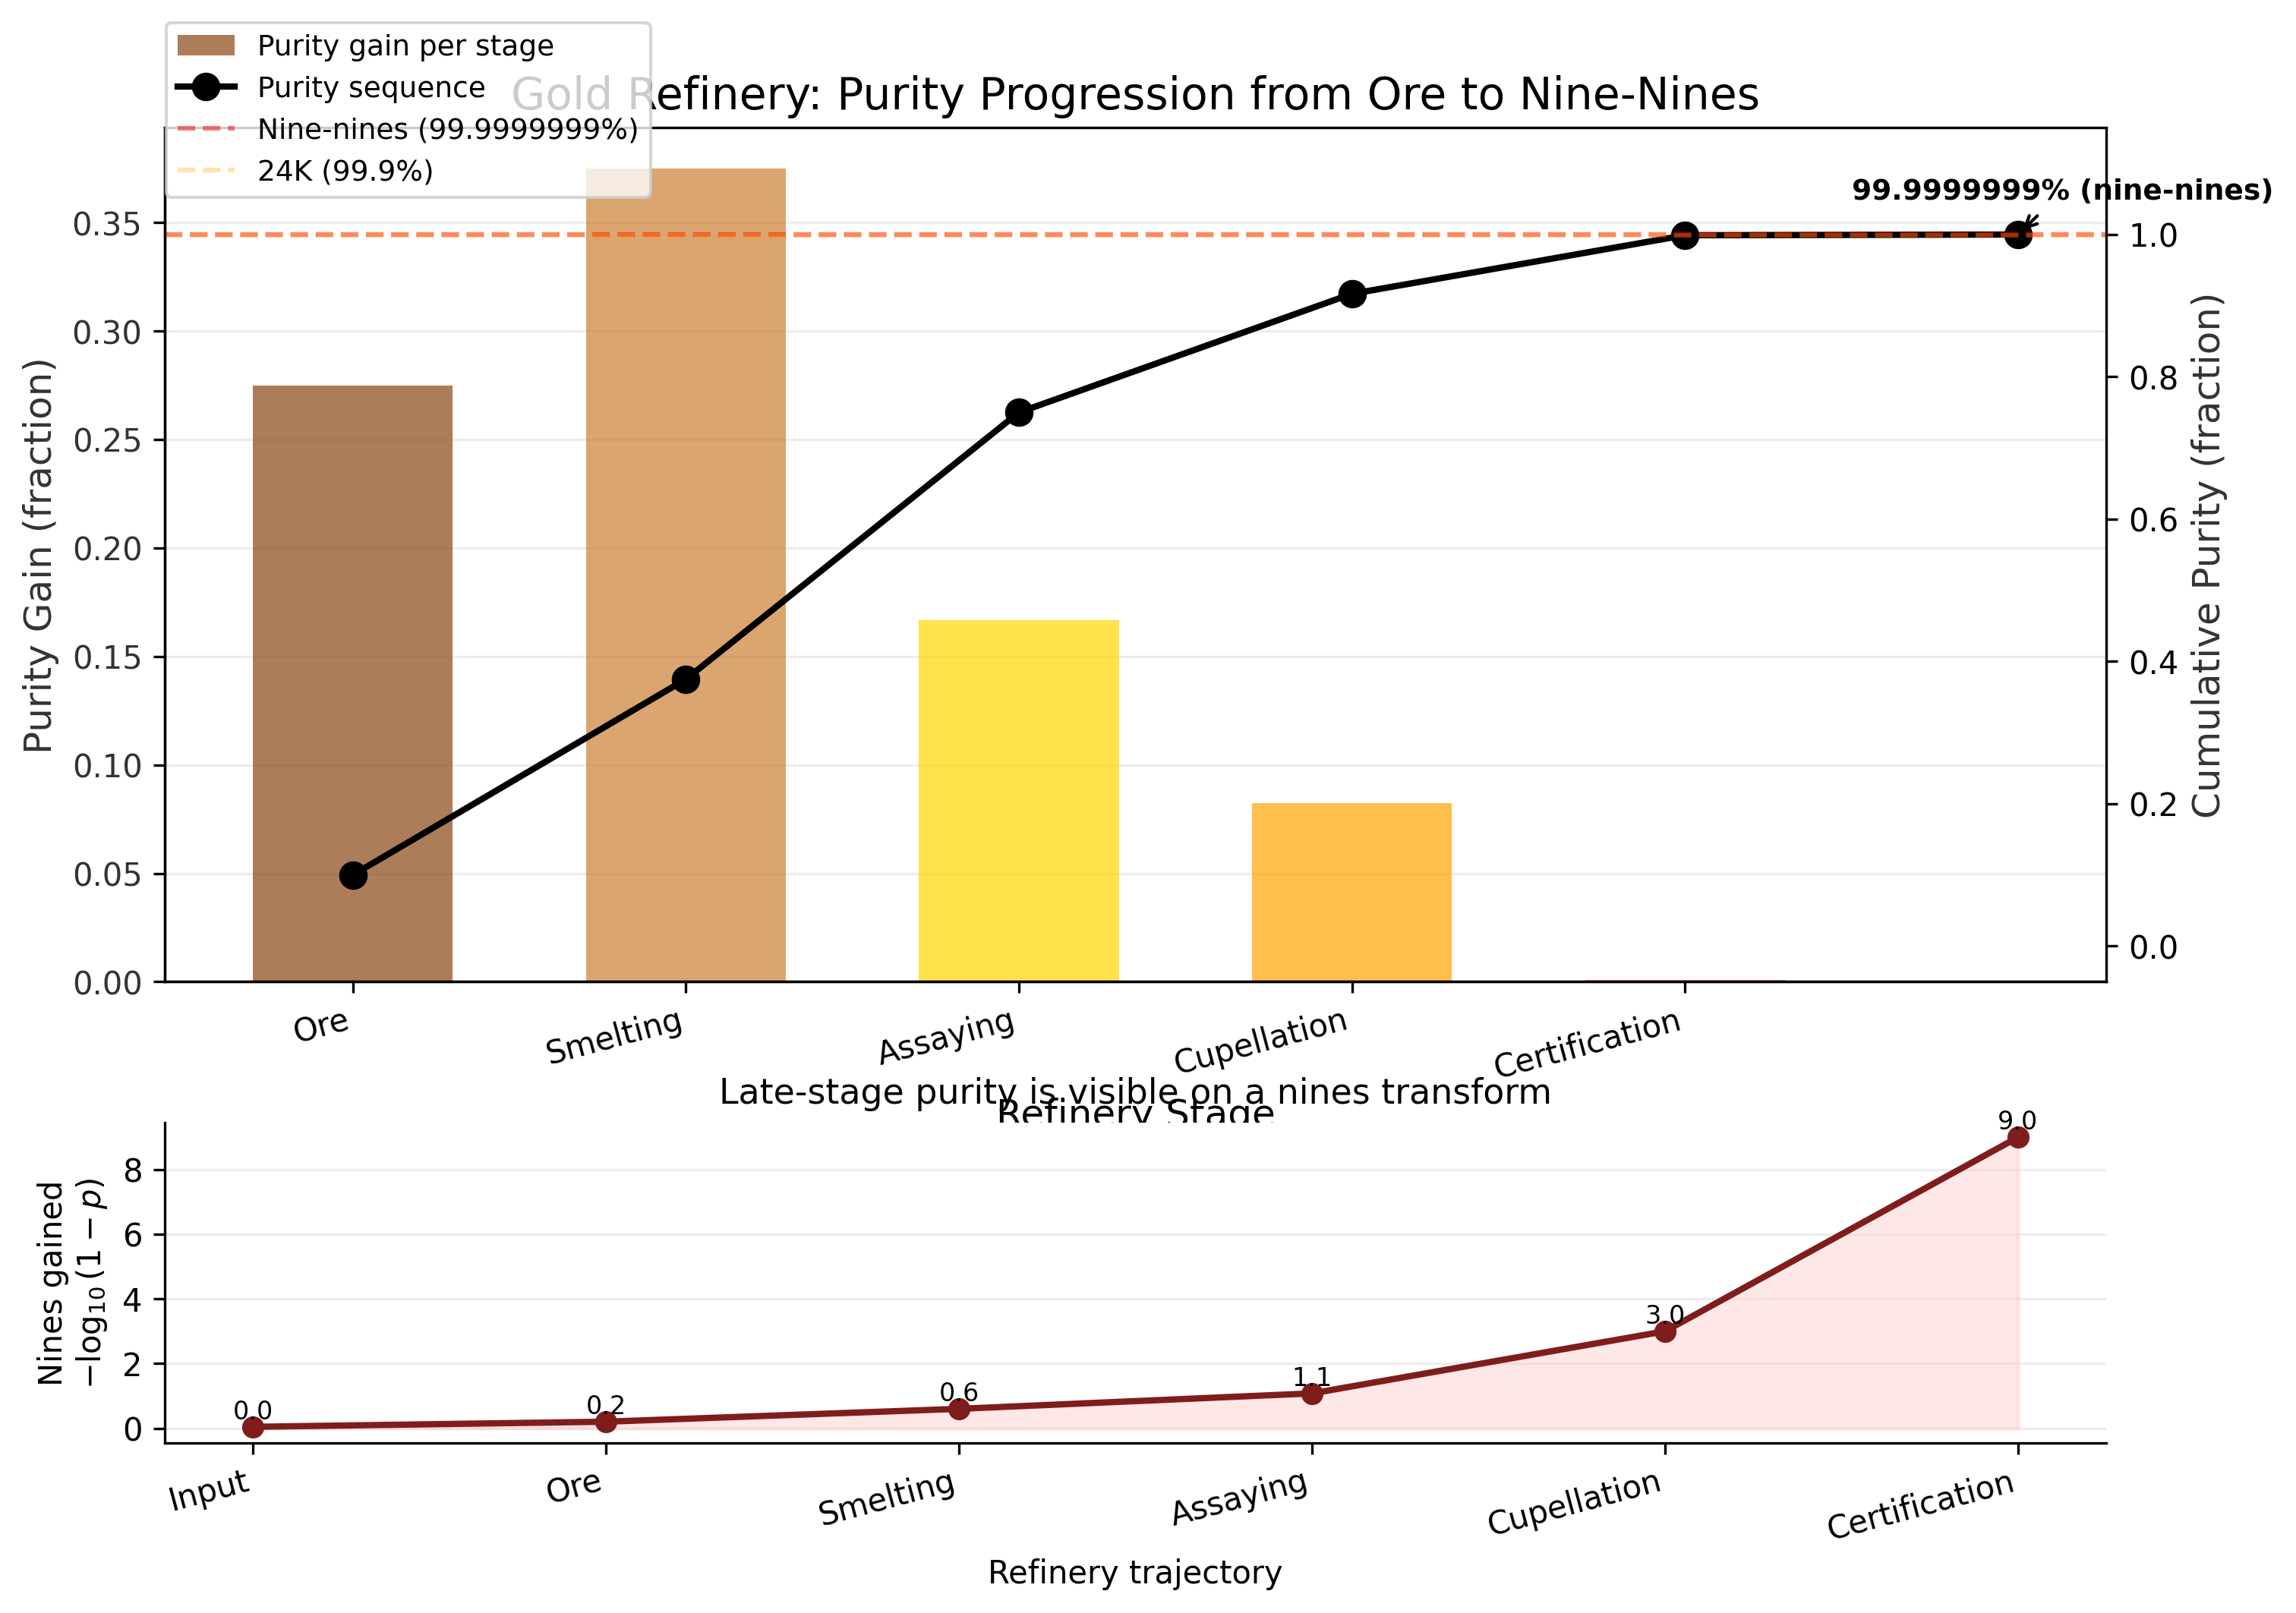
\includegraphics[keepaspectratio,alt={Purity progression across the five refinery stages from ore (9K) to nine-nines certification.}]{../figures/purity_progression.png}}
\caption{Purity progression across the five refinery stages from ore
(9K) to nine-nines certification.}\label{fig:purity_progression}
\end{figure}

{\def\LTcaptype{none} % do not increment counter
\begin{longtable}[]{@{}
  >{\raggedright\arraybackslash}p{(\linewidth - 8\tabcolsep) * \real{0.1750}}
  >{\raggedright\arraybackslash}p{(\linewidth - 8\tabcolsep) * \real{0.1500}}
  >{\raggedright\arraybackslash}p{(\linewidth - 8\tabcolsep) * \real{0.3500}}
  >{\raggedright\arraybackslash}p{(\linewidth - 8\tabcolsep) * \real{0.1750}}
  >{\raggedright\arraybackslash}p{(\linewidth - 8\tabcolsep) * \real{0.1500}}@{}}
\toprule\noalign{}
\begin{minipage}[b]{\linewidth}\raggedright
Stage
\end{minipage} & \begin{minipage}[b]{\linewidth}\raggedright
Name
\end{minipage} & \begin{minipage}[b]{\linewidth}\raggedright
Output purity
\end{minipage} & \begin{minipage}[b]{\linewidth}\raggedright
Karat
\end{minipage} & \begin{minipage}[b]{\linewidth}\raggedright
Gain
\end{minipage} \\
\midrule\noalign{}
\endhead
\bottomrule\noalign{}
\endlastfoot
1 & ore & 37.50\% & 9K & Extract raw gold-bearing ore from the earth \\
2 & smelting & 75.00\% & 18K & Heat ore to separate gold from slag and
dross \\
3 & assaying & 91.67\% & 22K & Test a sample to determine gold content
and impurities \\
4 & cupellation & 99.900\% & 24K & Refine by blowing air through molten
lead-gold alloy \\
5 & certification & 99.9999999\% (nine-nines) & 24K (nine-nines
certified) & Certify purity grade and stamp hallmark \\
\end{longtable}
}

\subsection{Karat grading scale}\label{karat-grading-scale}

\begin{figure}
\centering
\pandocbounded{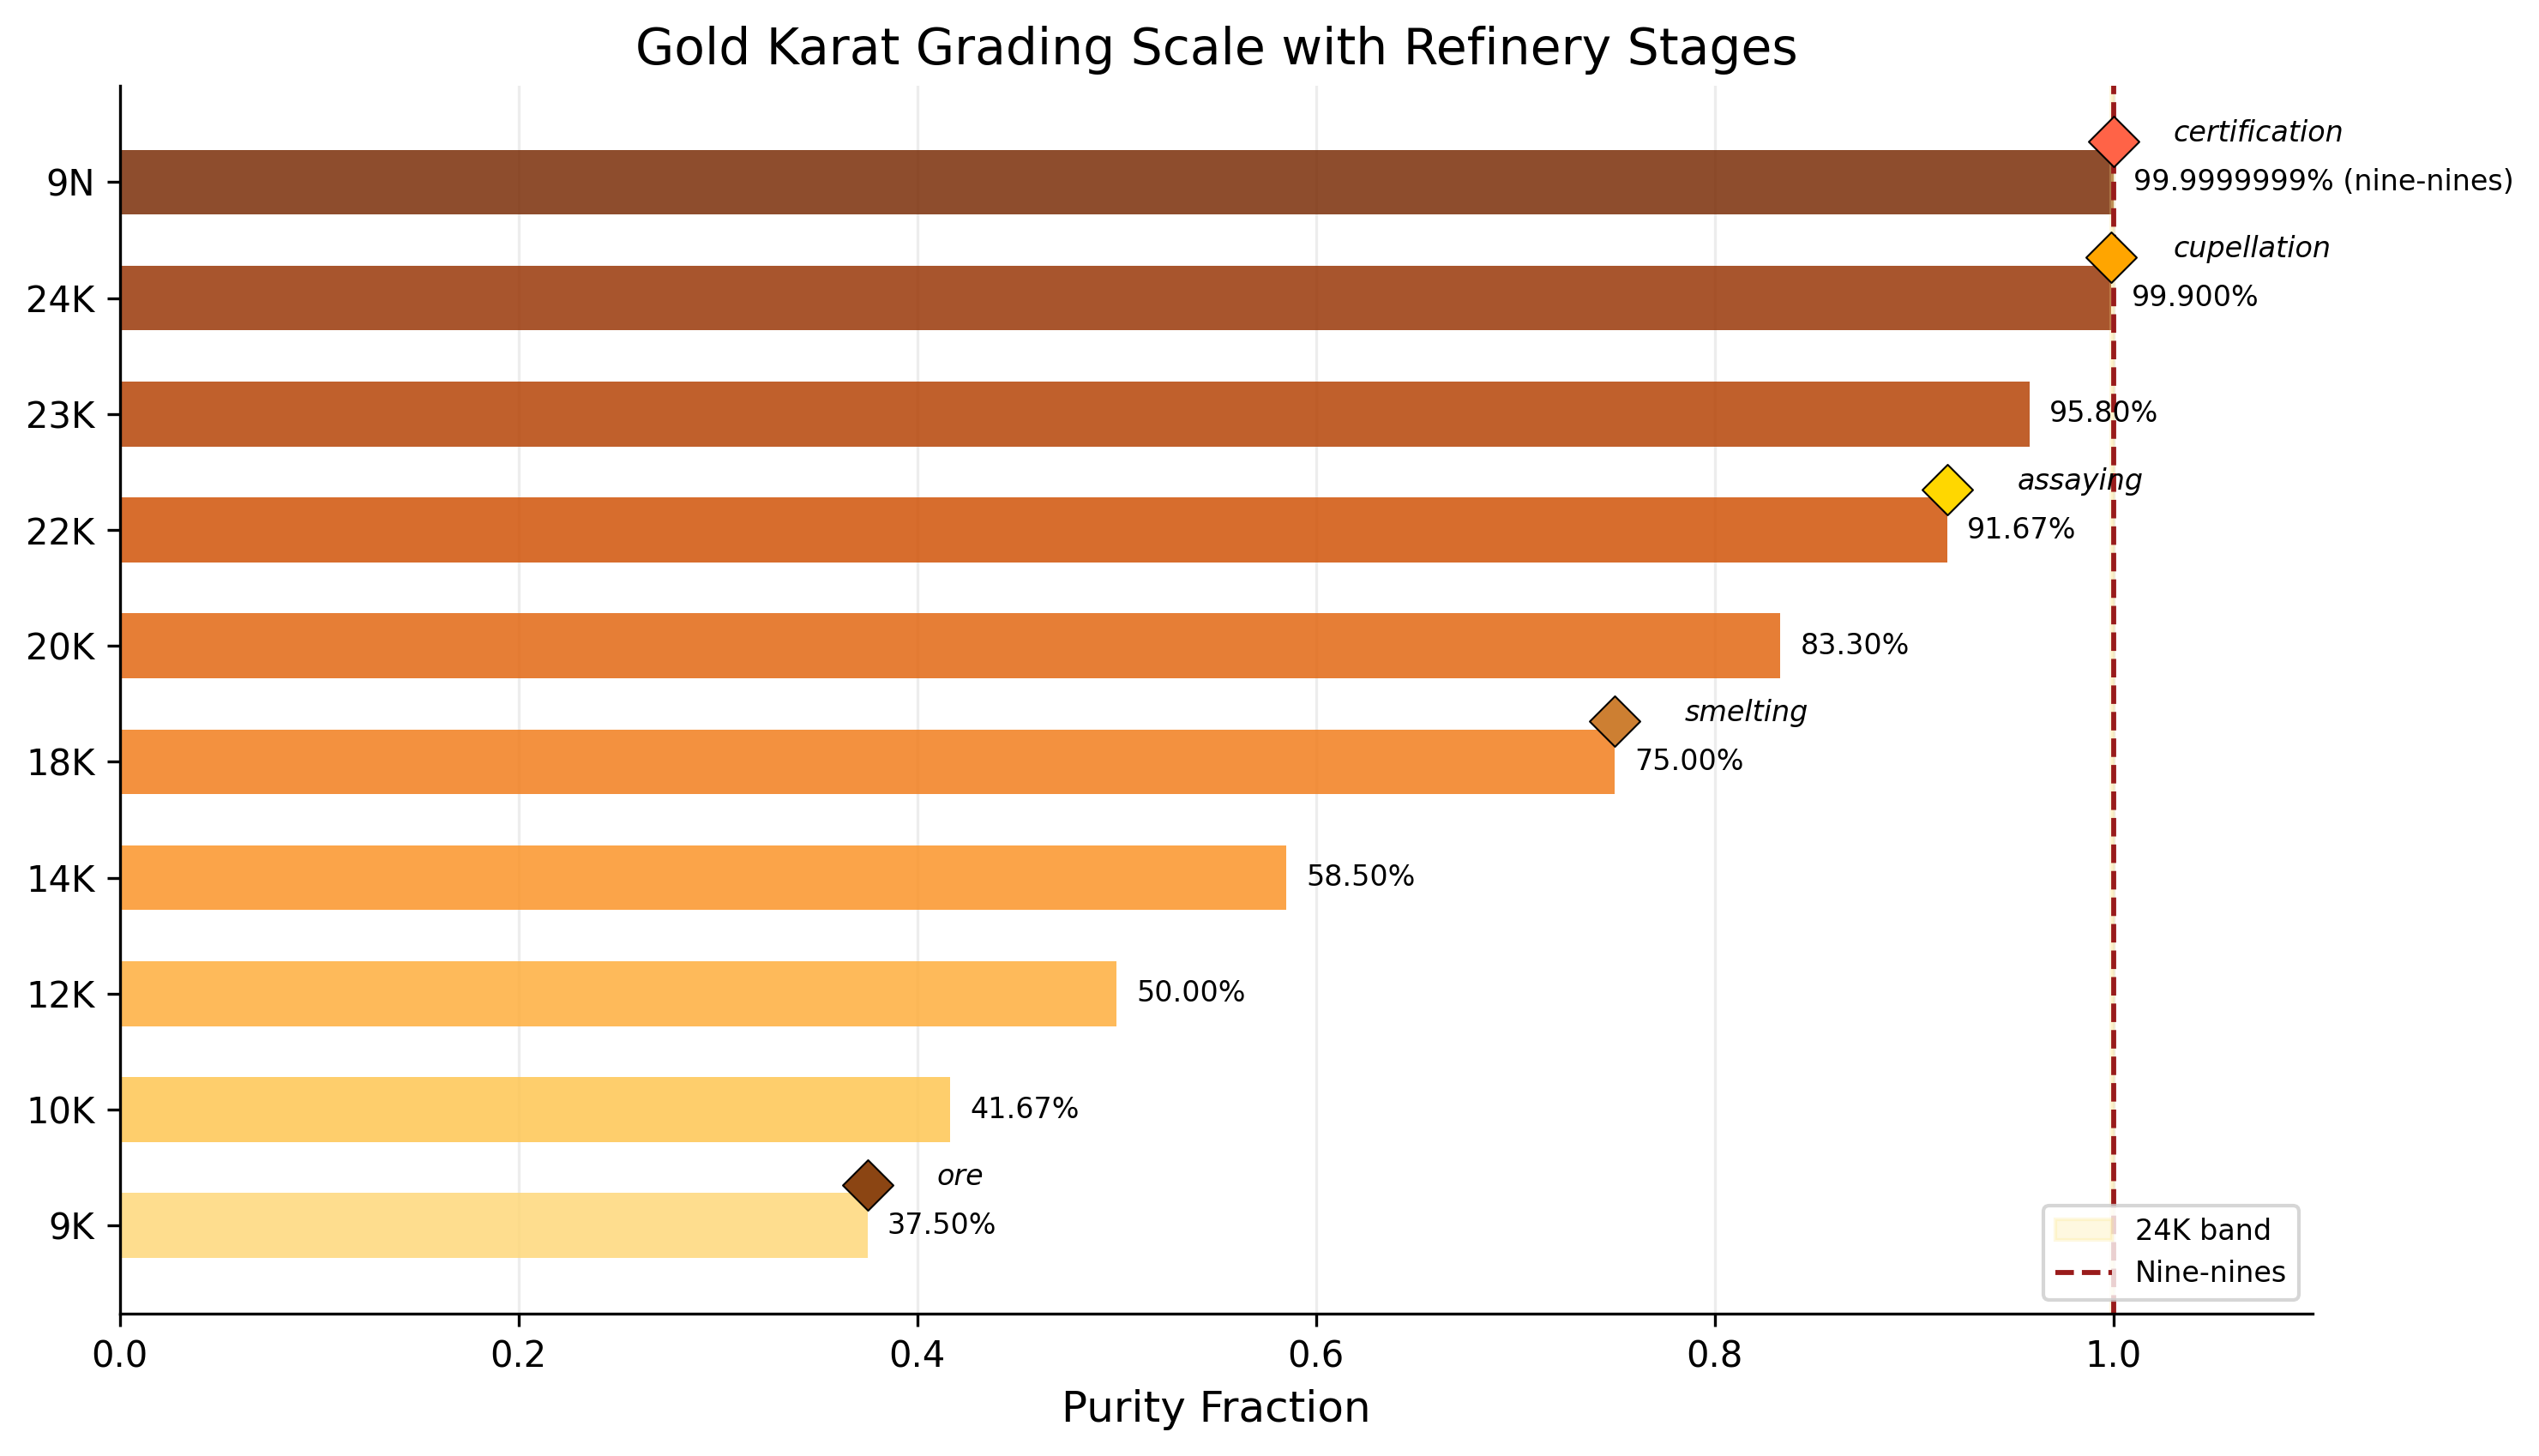
\includegraphics[keepaspectratio,alt={Gold karat grading scale (9K--24K + nine-nines) with refinery stage markers.}]{../figures/karat_grading.png}}
\caption{Gold karat grading scale (9K--24K + nine-nines) with refinery
stage markers.}\label{fig:karat_grading}
\end{figure}

\subsection{Final certification}\label{final-certification}

\begin{itemize}
\tightlist
\item
  \textbf{Final purity:} 99.9999999\% (nine-nines)
\item
  \textbf{Final karat:} 24K (nine-nines certified)
\item
  \textbf{Total purity gain:} 90.00\%
\item
  \textbf{Nine-nines certified:} Yes
\item
  \textbf{Nines count:} 9
\end{itemize}

\subsection{Seed-sensitivity results}\label{seed-sensitivity-results}

The expanded sensitivity study evaluated 1024 technical replicates of
the deterministic token pipeline over seeds 0--1023. It found 1024
unique token plans among 1024 runs, with 1 exact matches to the
canonical plan. Mean slot agreement was 20.62\% (SD 8.56\%; descriptive
95\% interval 20.09\%--21.14\%), with observed range 0.00\%--100.00\%.
The configured threshold rate was 36.43\% (score interval
33.53\%--39.42\%) at the 25\% agreement threshold. All configured
inventory values were observed (100.00\% coverage), which is a coverage
result for the token vocabulary rather than a quality result for the
manuscript.

The declared precision target requires at least 738 replicates under the
chosen bounded-metric formula; the realized radius is 4.24\%. The
deterministic bootstrap sensitivity interval for the mean is
20.10\%--21.11\% from 2000 resamples. Both intervals are conditional
technical summaries, not population estimates.

\begin{figure}
\centering
\pandocbounded{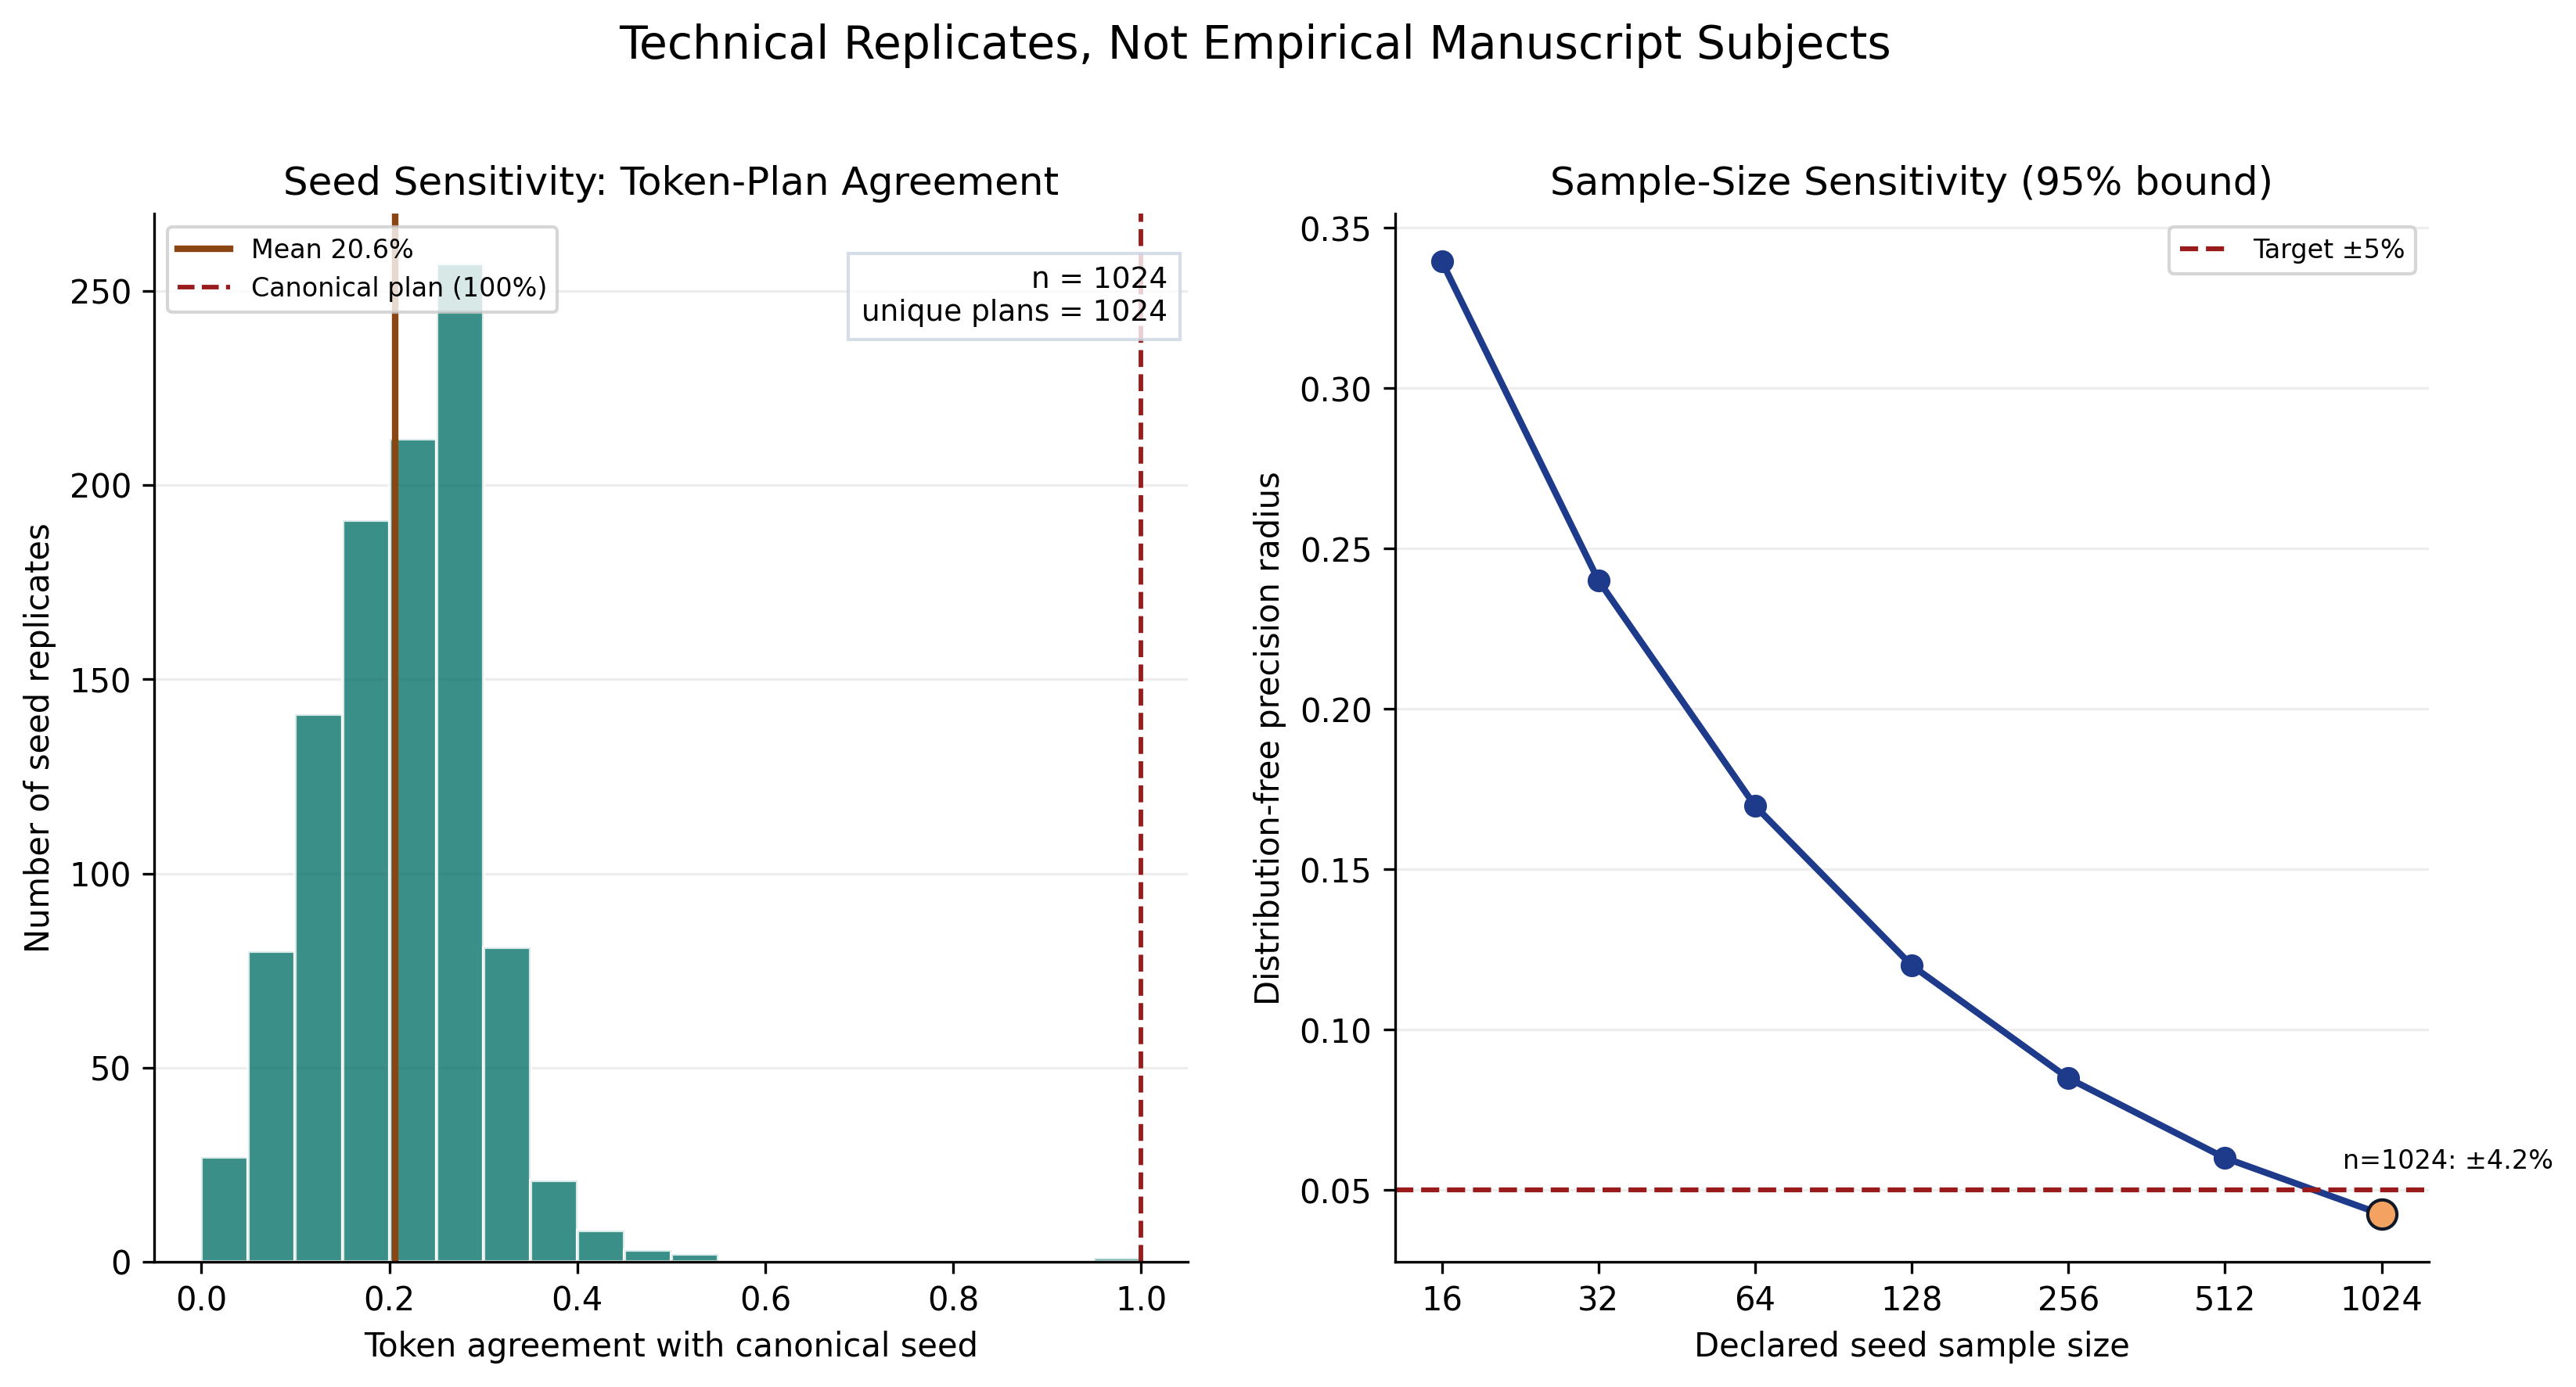
\includegraphics[keepaspectratio,alt={Seed-sensitivity distribution and the declared sample-size precision ladder for token-plan agreement.}]{../figures/seed_sensitivity.png}}
\caption{Seed-sensitivity distribution and the declared sample-size
precision ladder for token-plan agreement.}\label{fig:seed_sensitivity}
\end{figure}

The report is stored at \breaktt{output/data/seed\_sensitivity.json}.
These are technical replicates of one executable token pipeline, not
human participants, independent manuscripts, or evidence of external
manuscript quality. The sensitivity result therefore refines the
reproducibility claim: a fixed seed exactly regenerates a selected plan,
while neighboring seeds explore a wide deterministic outcome surface. It
does not justify treating token agreement as a reader-quality metric or
as evidence that one lexical choice is scientifically superior.

\subsection{Token plan summary}\label{token-plan-summary}

The mega-madlib engine generated 24 tokens from seed 431 across 8
lexicon categories.

\begin{figure}
\centering
\pandocbounded{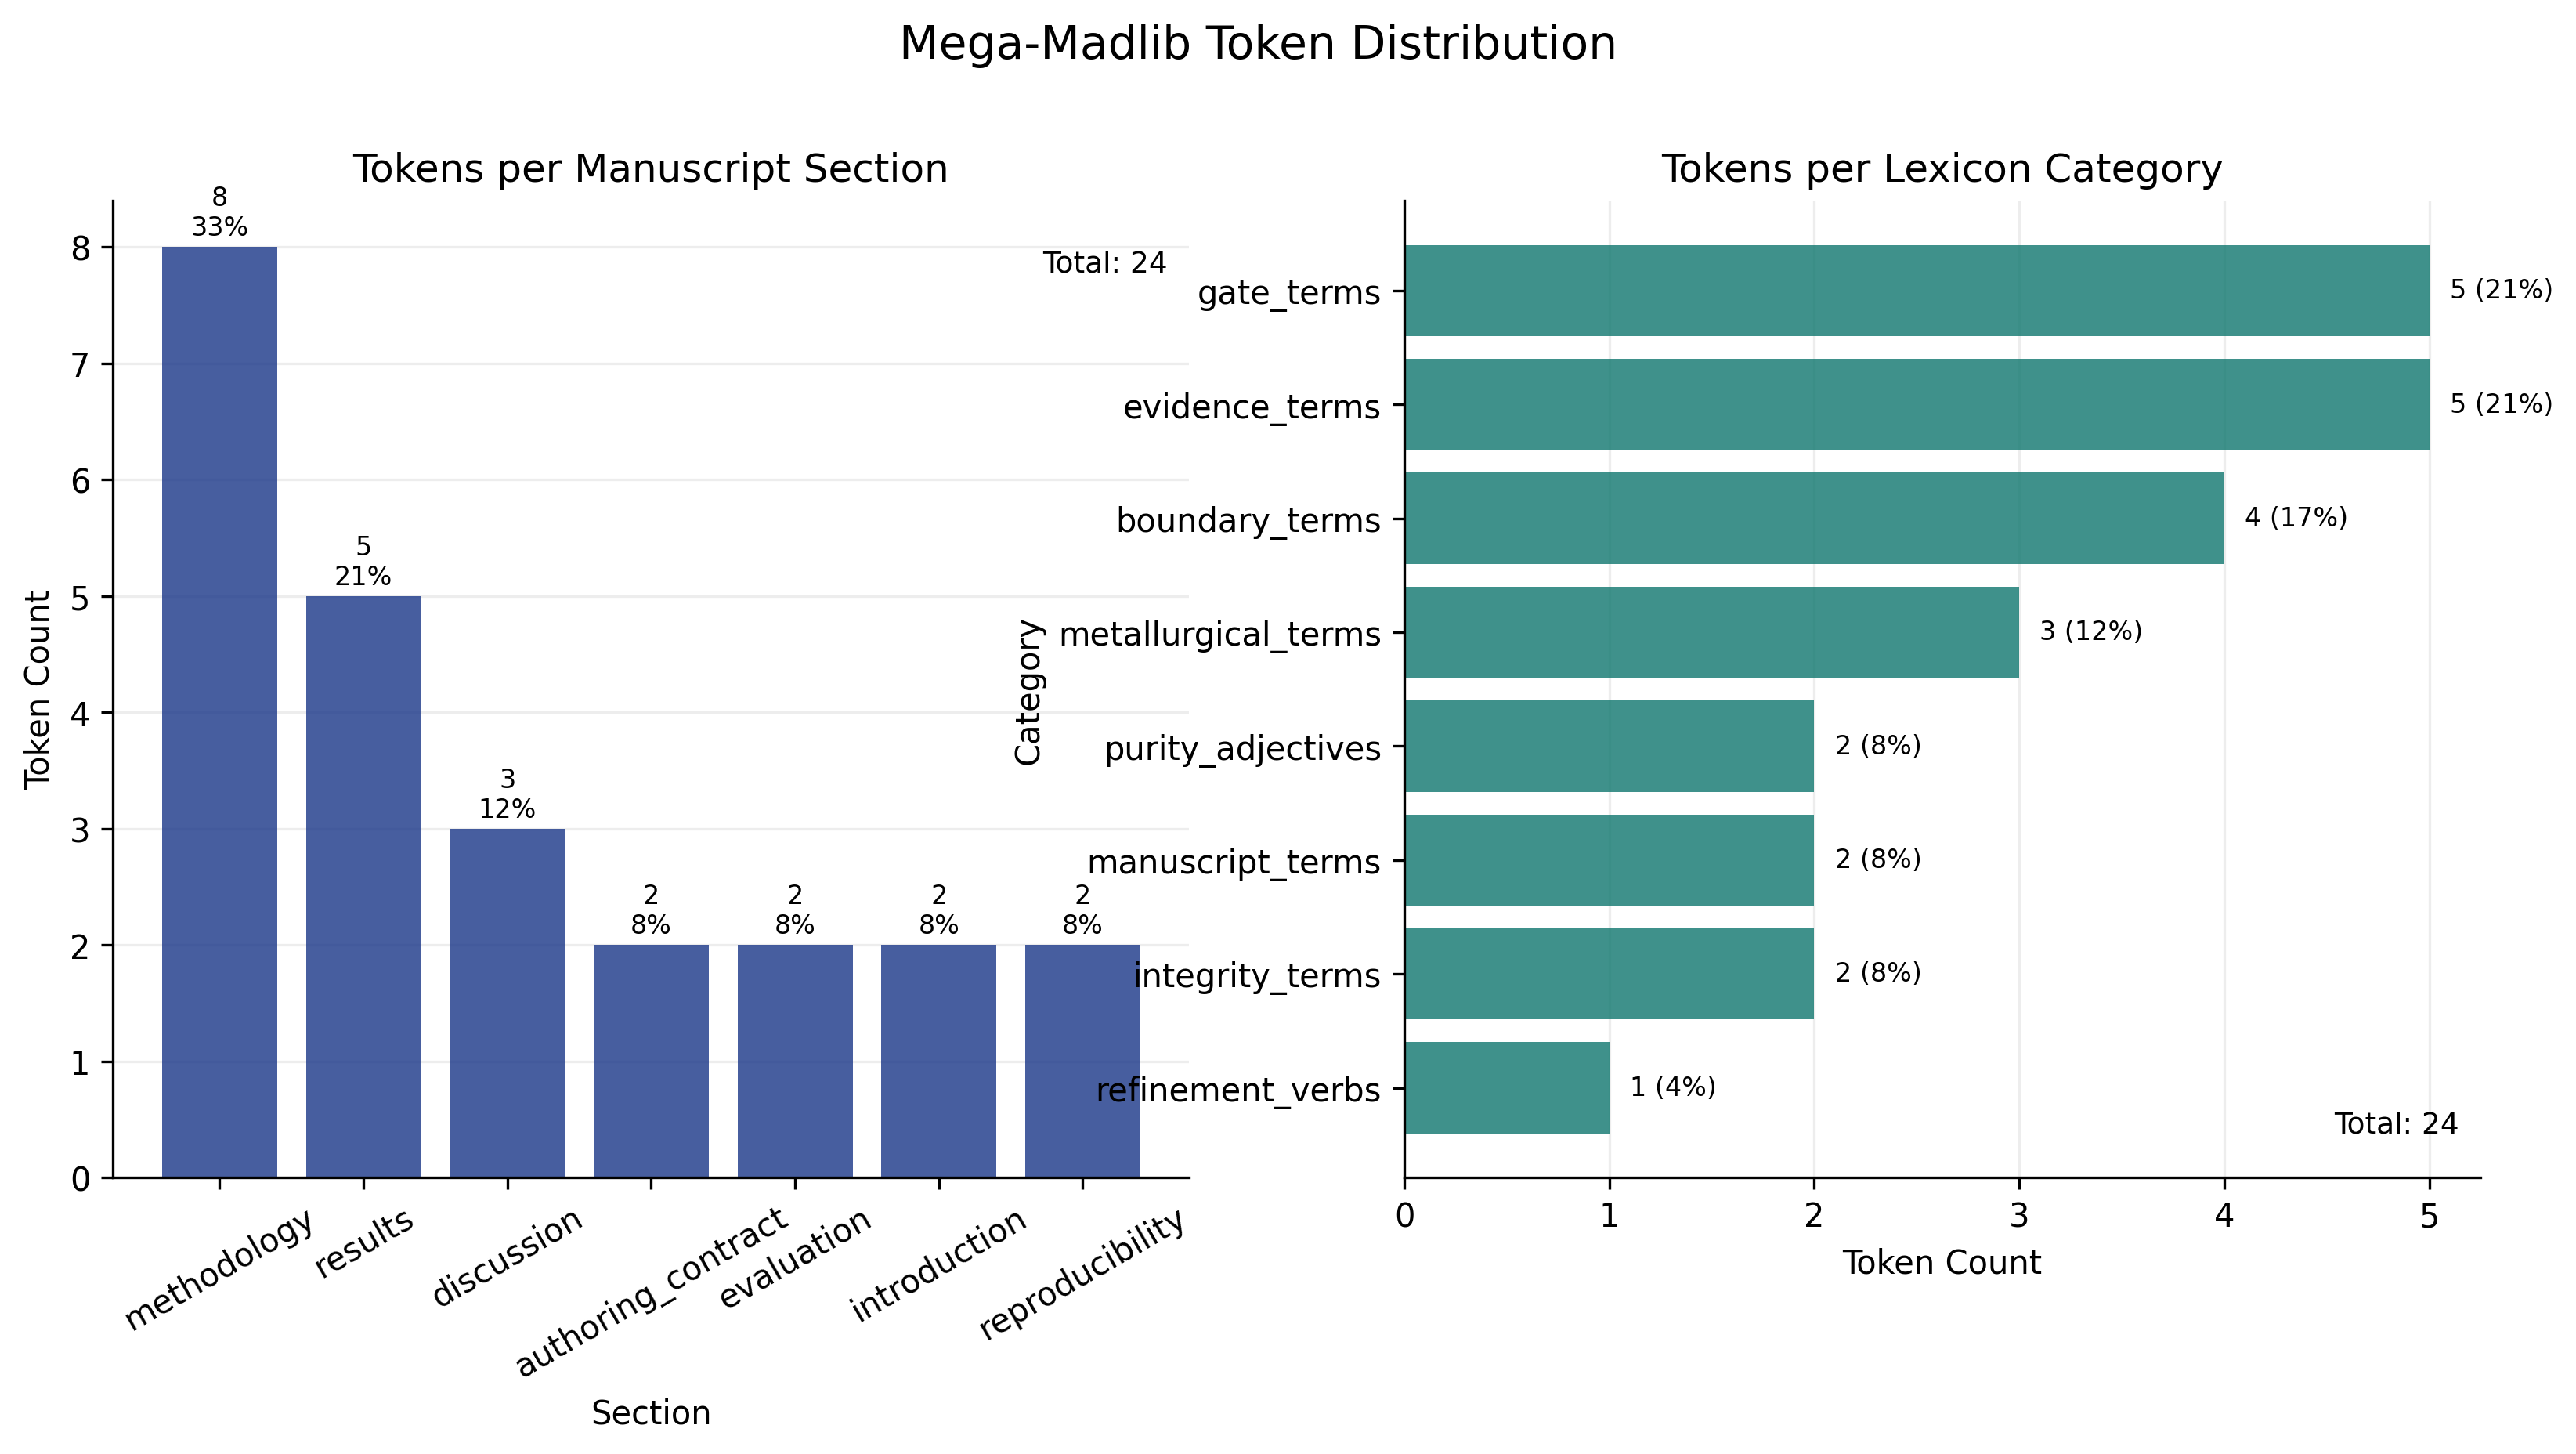
\includegraphics[keepaspectratio,alt={Mega-madlib token distribution across manuscript sections and lexicon categories.}]{../figures/token_density.png}}
\caption{Mega-madlib token distribution across manuscript sections and
lexicon categories.}\label{fig:token_density}
\end{figure}

\subsubsection{Category distribution}\label{category-distribution}

{\def\LTcaptype{none} % do not increment counter
\begin{longtable}[]{@{}ll@{}}
\toprule\noalign{}
Category & Count \\
\midrule\noalign{}
\endhead
\bottomrule\noalign{}
\endlastfoot
boundary\_terms & 4 \\
evidence\_terms & 5 \\
gate\_terms & 5 \\
integrity\_terms & 2 \\
manuscript\_terms & 2 \\
metallurgical\_terms & 3 \\
purity\_adjectives & 2 \\
refinement\_verbs & 1 \\
\end{longtable}
}

\subsubsection{Section distribution}\label{section-distribution}

{\def\LTcaptype{none} % do not increment counter
\begin{longtable}[]{@{}ll@{}}
\toprule\noalign{}
Section & Token count \\
\midrule\noalign{}
\endhead
\bottomrule\noalign{}
\endlastfoot
authoring\_contract & 2 \\
discussion & 3 \\
evaluation & 2 \\
introduction & 2 \\
methodology & 8 \\
reproducibility & 2 \\
results & 5 \\
\end{longtable}
}

\subsubsection{Provenance trace}\label{provenance-trace}

{\def\LTcaptype{none} % do not increment counter
\begin{longtable}[]{@{}
  >{\raggedright\arraybackslash}p{(\linewidth - 8\tabcolsep) * \real{0.2273}}
  >{\raggedright\arraybackslash}p{(\linewidth - 8\tabcolsep) * \real{0.2273}}
  >{\raggedright\arraybackslash}p{(\linewidth - 8\tabcolsep) * \real{0.1591}}
  >{\raggedright\arraybackslash}p{(\linewidth - 8\tabcolsep) * \real{0.2045}}
  >{\raggedright\arraybackslash}p{(\linewidth - 8\tabcolsep) * \real{0.1818}}@{}}
\toprule\noalign{}
\begin{minipage}[b]{\linewidth}\raggedright
Variable
\end{minipage} & \begin{minipage}[b]{\linewidth}\raggedright
Category
\end{minipage} & \begin{minipage}[b]{\linewidth}\raggedright
Value
\end{minipage} & \begin{minipage}[b]{\linewidth}\raggedright
Section
\end{minipage} & \begin{minipage}[b]{\linewidth}\raggedright
Source
\end{minipage} \\
\midrule\noalign{}
\endhead
\bottomrule\noalign{}
\endlastfoot
AUTHORING\_BOUNDARY\_TERM\_1 & boundary\_terms & analogy boundary &
authoring\_contract &
manuscript/config.yaml\#gold\_refinement.lexicon.boundary\_terms{[}1{]} \\
AUTHORING\_BOUNDARY\_TERM\_2 & boundary\_terms & non-claim &
authoring\_contract &
manuscript/config.yaml\#gold\_refinement.lexicon.boundary\_terms{[}4{]} \\
DISCUSSION\_BOUNDARY\_TERM\_1 & boundary\_terms & fork obligation &
discussion &
manuscript/config.yaml\#gold\_refinement.lexicon.boundary\_terms{[}2{]} \\
DISCUSSION\_BOUNDARY\_TERM\_2 & boundary\_terms & domain validator &
discussion &
manuscript/config.yaml\#gold\_refinement.lexicon.boundary\_terms{[}3{]} \\
DISCUSSION\_REFINEMENT\_VERB & refinement\_verbs & smelting & discussion
&
manuscript/config.yaml\#gold\_refinement.lexicon.refinement\_verbs{[}3{]} \\
EVALUATION\_GATE\_TERM\_1 & gate\_terms & prerender & evaluation &
manuscript/config.yaml\#gold\_refinement.lexicon.gate\_terms{[}0{]} \\
EVALUATION\_GATE\_TERM\_2 & gate\_terms & citation validation &
evaluation &
manuscript/config.yaml\#gold\_refinement.lexicon.gate\_terms{[}3{]} \\
INTRO\_INTEGRITY\_TERM\_1 & integrity\_terms & source tier &
introduction &
manuscript/config.yaml\#gold\_refinement.lexicon.integrity\_terms{[}1{]} \\
INTRO\_INTEGRITY\_TERM\_2 & integrity\_terms & evidence spine &
introduction &
manuscript/config.yaml\#gold\_refinement.lexicon.integrity\_terms{[}0{]} \\
METHOD\_GATE\_TERM\_1 & gate\_terms & evidence validation & methodology
& manuscript/config.yaml\#gold\_refinement.lexicon.gate\_terms{[}1{]} \\
METHOD\_GATE\_TERM\_2 & gate\_terms & figure registry check &
methodology &
manuscript/config.yaml\#gold\_refinement.lexicon.gate\_terms{[}2{]} \\
METHOD\_GATE\_TERM\_3 & gate\_terms & citation validation & methodology
& manuscript/config.yaml\#gold\_refinement.lexicon.gate\_terms{[}3{]} \\
METHOD\_MANUSCRIPT\_TERM\_1 & manuscript\_terms & evidence & methodology
&
manuscript/config.yaml\#gold\_refinement.lexicon.manuscript\_terms{[}4{]} \\
METHOD\_MANUSCRIPT\_TERM\_2 & manuscript\_terms & evidence & methodology
&
manuscript/config.yaml\#gold\_refinement.lexicon.manuscript\_terms{[}4{]} \\
METHOD\_METAL\_TERM\_1 & metallurgical\_terms & assaying & methodology &
manuscript/config.yaml\#gold\_refinement.lexicon.metallurgical\_terms{[}1{]} \\
METHOD\_METAL\_TERM\_2 & metallurgical\_terms & parting & methodology &
manuscript/config.yaml\#gold\_refinement.lexicon.metallurgical\_terms{[}3{]} \\
METHOD\_METAL\_TERM\_3 & metallurgical\_terms & smelting & methodology &
manuscript/config.yaml\#gold\_refinement.lexicon.metallurgical\_terms{[}2{]} \\
REPRO\_EVIDENCE\_TERM\_1 & evidence\_terms & fact registry &
reproducibility &
manuscript/config.yaml\#gold\_refinement.lexicon.evidence\_terms{[}0{]} \\
REPRO\_EVIDENCE\_TERM\_2 & evidence\_terms & figure registry &
reproducibility &
manuscript/config.yaml\#gold\_refinement.lexicon.evidence\_terms{[}3{]} \\
RESULTS\_EVIDENCE\_TERM\_1 & evidence\_terms & artifact manifest &
results &
manuscript/config.yaml\#gold\_refinement.lexicon.evidence\_terms{[}1{]} \\
RESULTS\_EVIDENCE\_TERM\_2 & evidence\_terms & figure registry & results
&
manuscript/config.yaml\#gold\_refinement.lexicon.evidence\_terms{[}3{]} \\
RESULTS\_EVIDENCE\_TERM\_3 & evidence\_terms & token provenance &
results &
manuscript/config.yaml\#gold\_refinement.lexicon.evidence\_terms{[}4{]} \\
RESULTS\_PURITY\_ADJ\_1 & purity\_adjectives & unrefined & results &
manuscript/config.yaml\#gold\_refinement.lexicon.purity\_adjectives{[}0{]} \\
RESULTS\_PURITY\_ADJ\_2 & purity\_adjectives & purified & results &
manuscript/config.yaml\#gold\_refinement.lexicon.purity\_adjectives{[}1{]} \\
\end{longtable}
}

Selected purity adjectives for this section: unrefined, purified.
Selected evidence terms: artifact manifest, figure registry, token
provenance.

\subsection{Provenance flow}\label{provenance-flow}

The provenance flow in fig.~\ref{fig:provenance_sankey} makes the
refinement analogy auditable as a directed source path rather than a
decorative metaphor. The graph starts from the same stage sequence used
in the purity table and carries that sequence forward to certification,
with edge width proportional to the purity gain owned by
\breaktt{src/refinery.py::run\_refinery}. A reader can therefore ask
where each improvement enters the pipeline and whether it is supported
by the same source that generated the reported purity numbers.

The main result is structural: certification is not allowed to appear as
a terminal label detached from the intermediate stages. It is only
reached after the upstream transformations have been generated, ordered,
and connected. This matters for the manuscript contract because
provenance is doing more than recording file paths. It is preserving
causal custody from raw material through assay and final certification,
so a later change to the stage model must move through the same graph,
table, and validation surfaces.

\begin{figure}
\centering
\pandocbounded{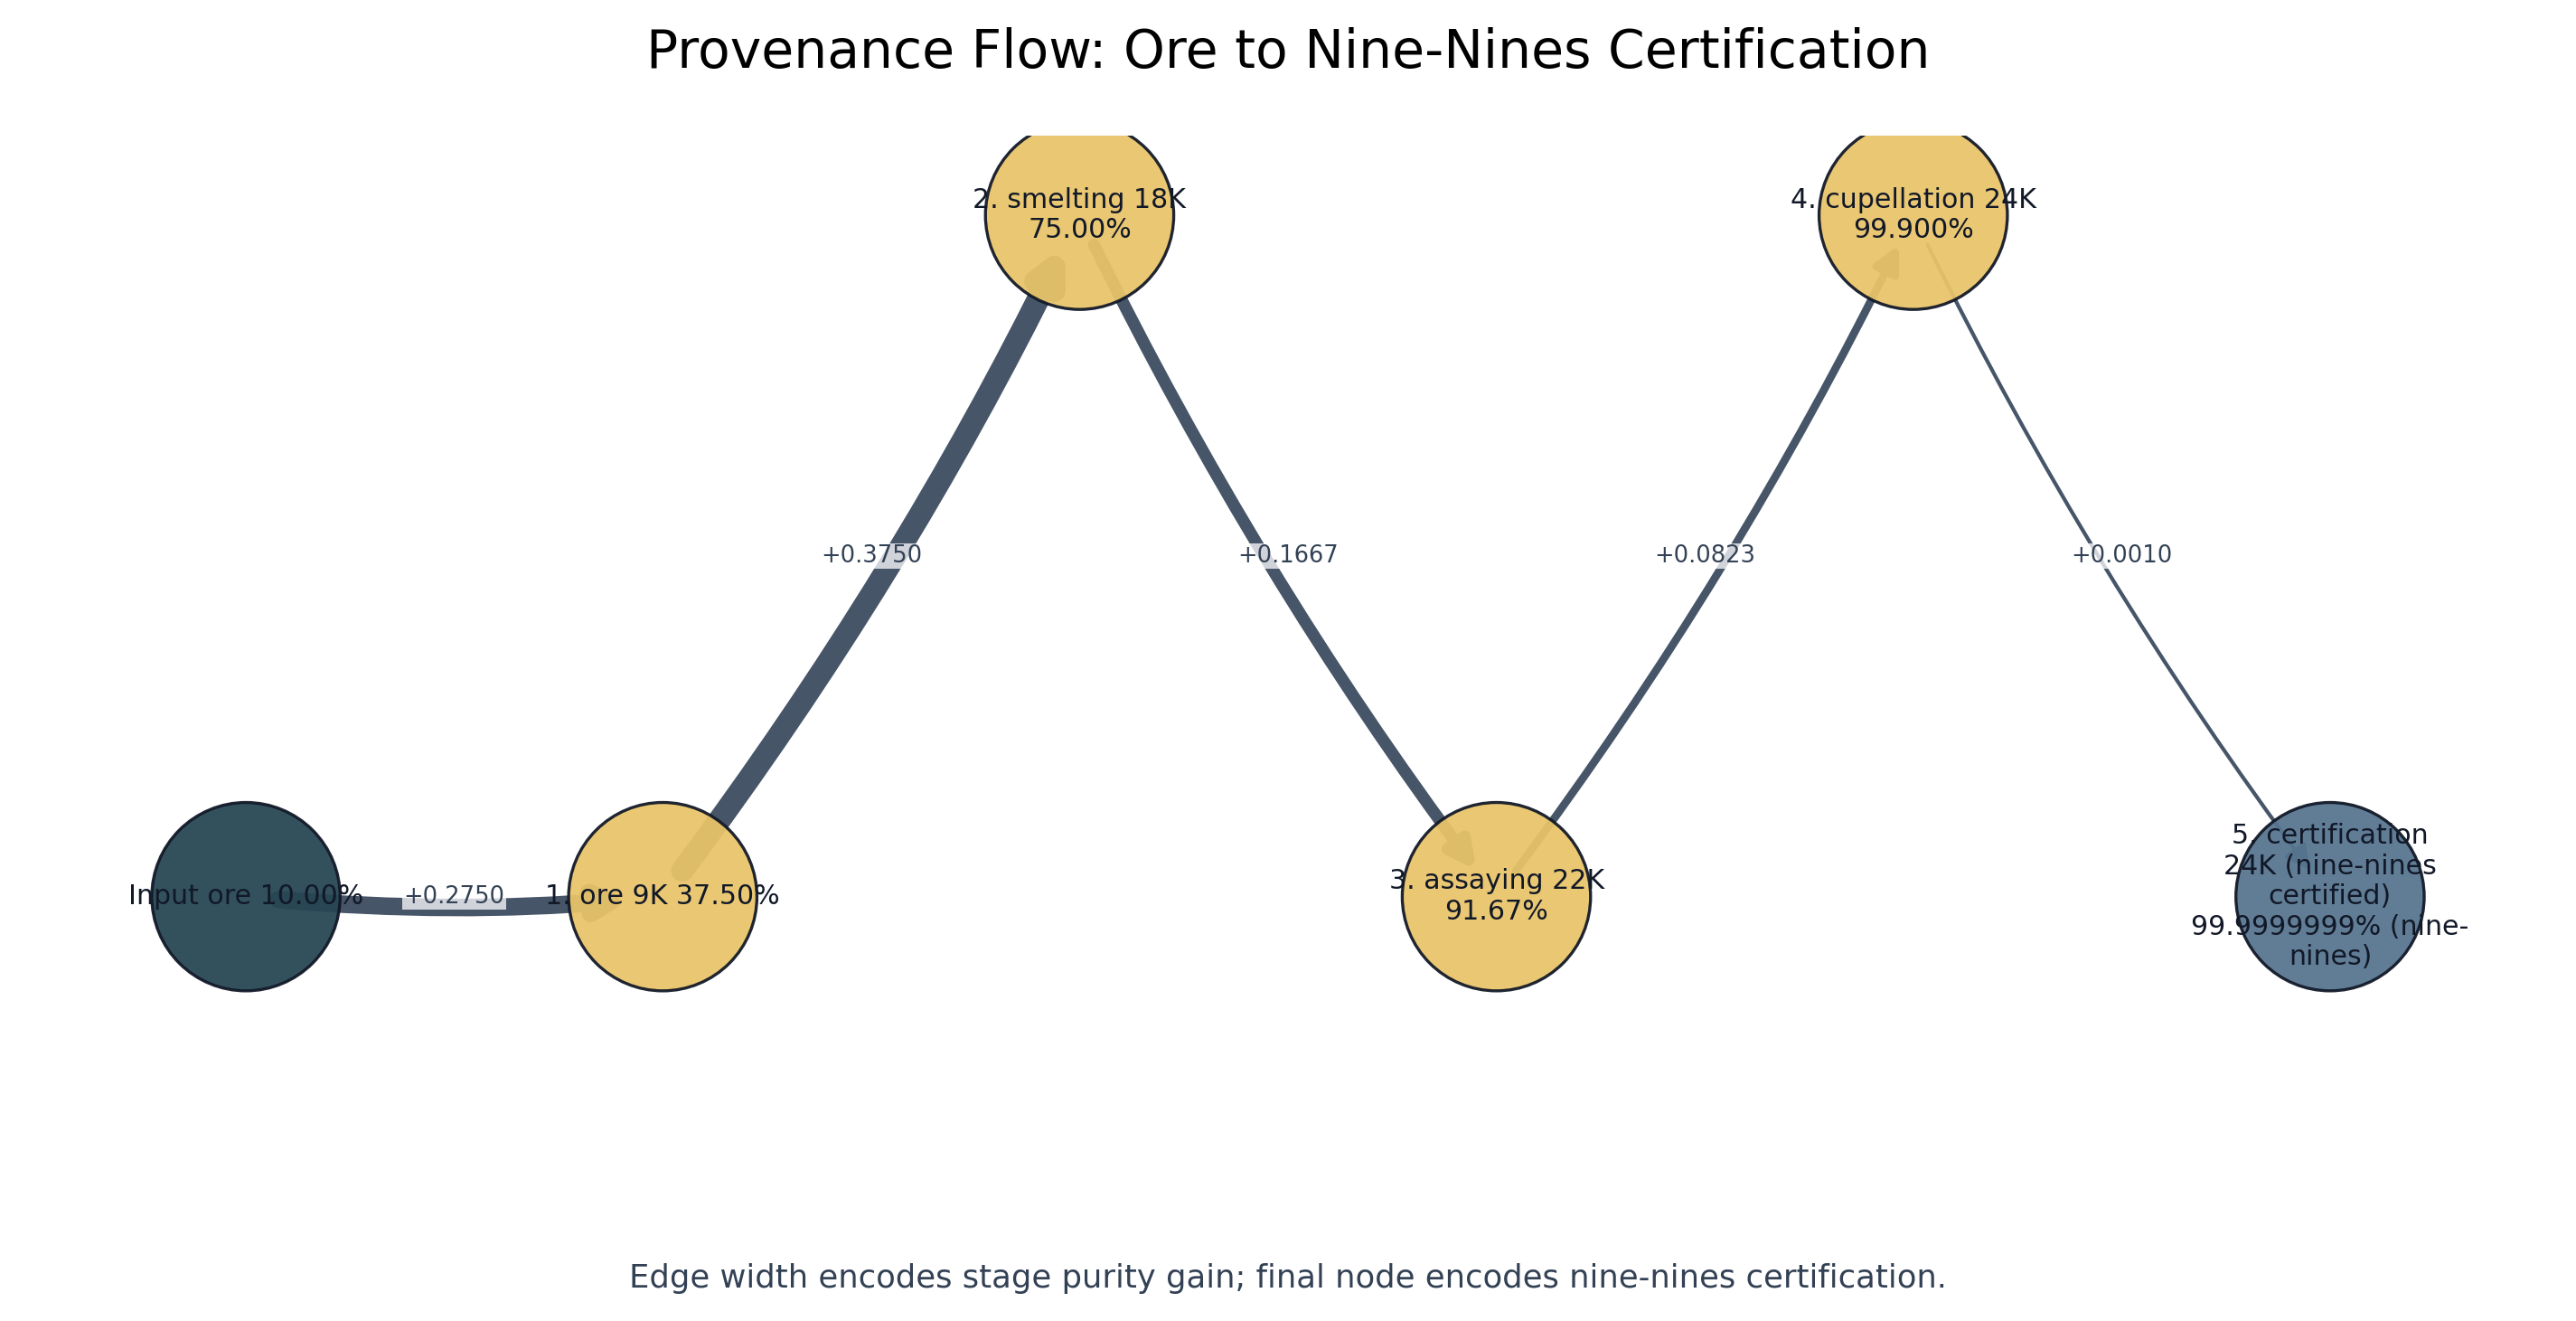
\includegraphics[keepaspectratio,alt={Provenance trace: ore \texorpdfstring{\ensuremath{\to}}{->} stages \texorpdfstring{\ensuremath{\to}}{->} certification purity flow.}]{../figures/provenance_sankey.png}}
\caption{Provenance trace: ore \texorpdfstring{\ensuremath{\to}}{->} stages \texorpdfstring{\ensuremath{\to}}{->} certification purity
flow.}\label{fig:provenance_sankey}
\end{figure}

\subsection{Purity vs claim support}\label{purity-vs-claim-support}

The purity-versus-claim-support view in
fig.~\ref{fig:purity_claim_scatter} places two differently scoped
measurements on explicit axes: stage output purity on the horizontal
axis and the single project-level contribution-claim assay on the
vertical axis. The same observed support rate is therefore repeated
across stages. The figure does not fabricate a stagewise claim-support
trajectory from a project-level aggregate.

In the current generated assay, 10 of 10 contribution claims are
supported (100.00\%). The plot is diagnostic rather than correlational:
five stage states and one ledger-level rate do not constitute
independent observations suitable for association testing. Its purpose
is to reveal disagreement between a late refinery state and weak overall
claim support without combining the two into one score.

\begin{figure}
\centering
\pandocbounded{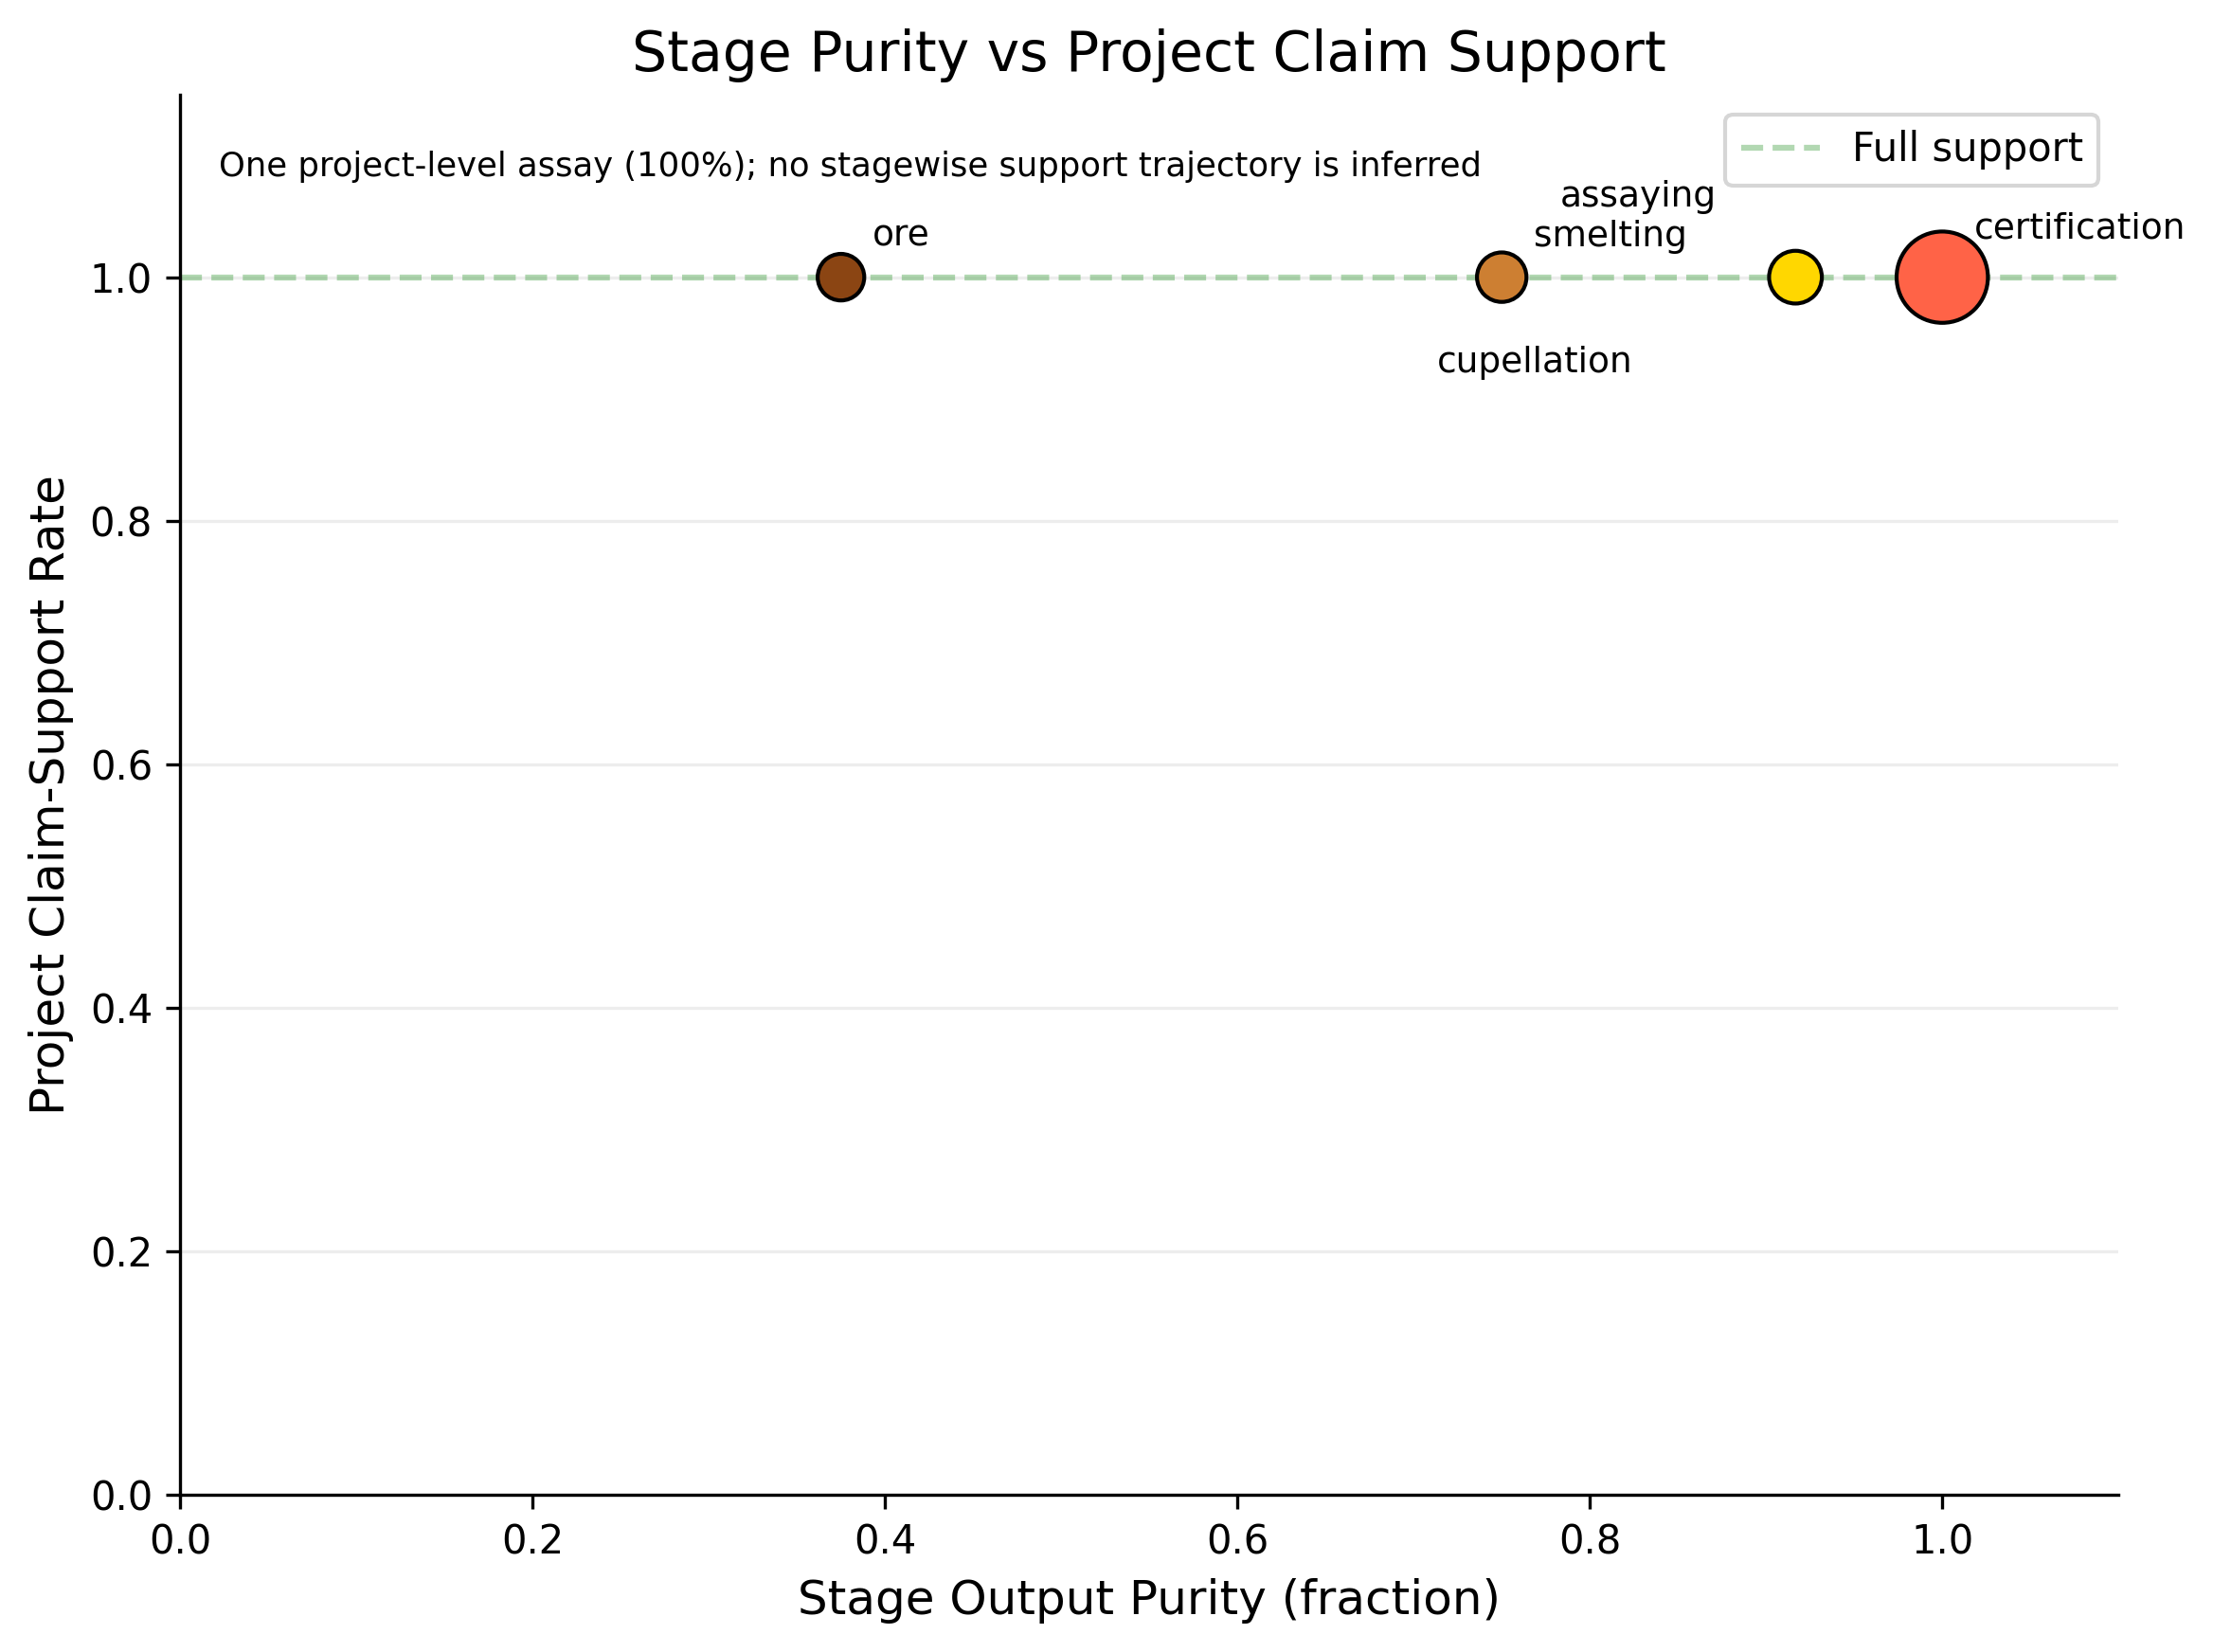
\includegraphics[keepaspectratio,alt={Stage purity plotted against the single project-level claim-support assay.}]{../figures/purity_claim_scatter.png}}
\caption{Stage purity plotted against the single project-level
claim-support assay.}\label{fig:purity_claim_scatter}
\end{figure}

\subsection{Token selection
sensitivity}\label{token-selection-sensitivity}

The token selection heatmap in fig.~\ref{fig:token_heatmap} turns the
mega-madlib engine into an inspectable sensitivity surface. The
manuscript uses seed 431 for the reported token plan, but the figure
asks a neighboring question: how do selected inventory indices move when
seeds and lexicon categories vary? This is not a stochastic robustness
claim. It is a deterministic audit of the digest rule in
\breaktt{src/composition.py::generate\_token\_plan} against the
configured lexicon inventories in \breaktt{manuscript/config.yaml}.

This view separates three issues that prose alone tends to blur. First,
token injection is reproducible: the same seed and inventory generate
the same choices. Second, the available vocabulary is a real input
surface: a thin or unbalanced category would be visible as a constrained
selection band. Third, render-time hydration is not silently sampling
new language. The heatmap therefore protects the manuscript from a
common generative-writing failure mode, where a polished section appears
stable but its wording is actually controlled by hidden or late-bound
choices. The result is a sensitivity check on authoring machinery, not a
claim that any particular synonym is scientifically superior.

\begin{figure}
\centering
\pandocbounded{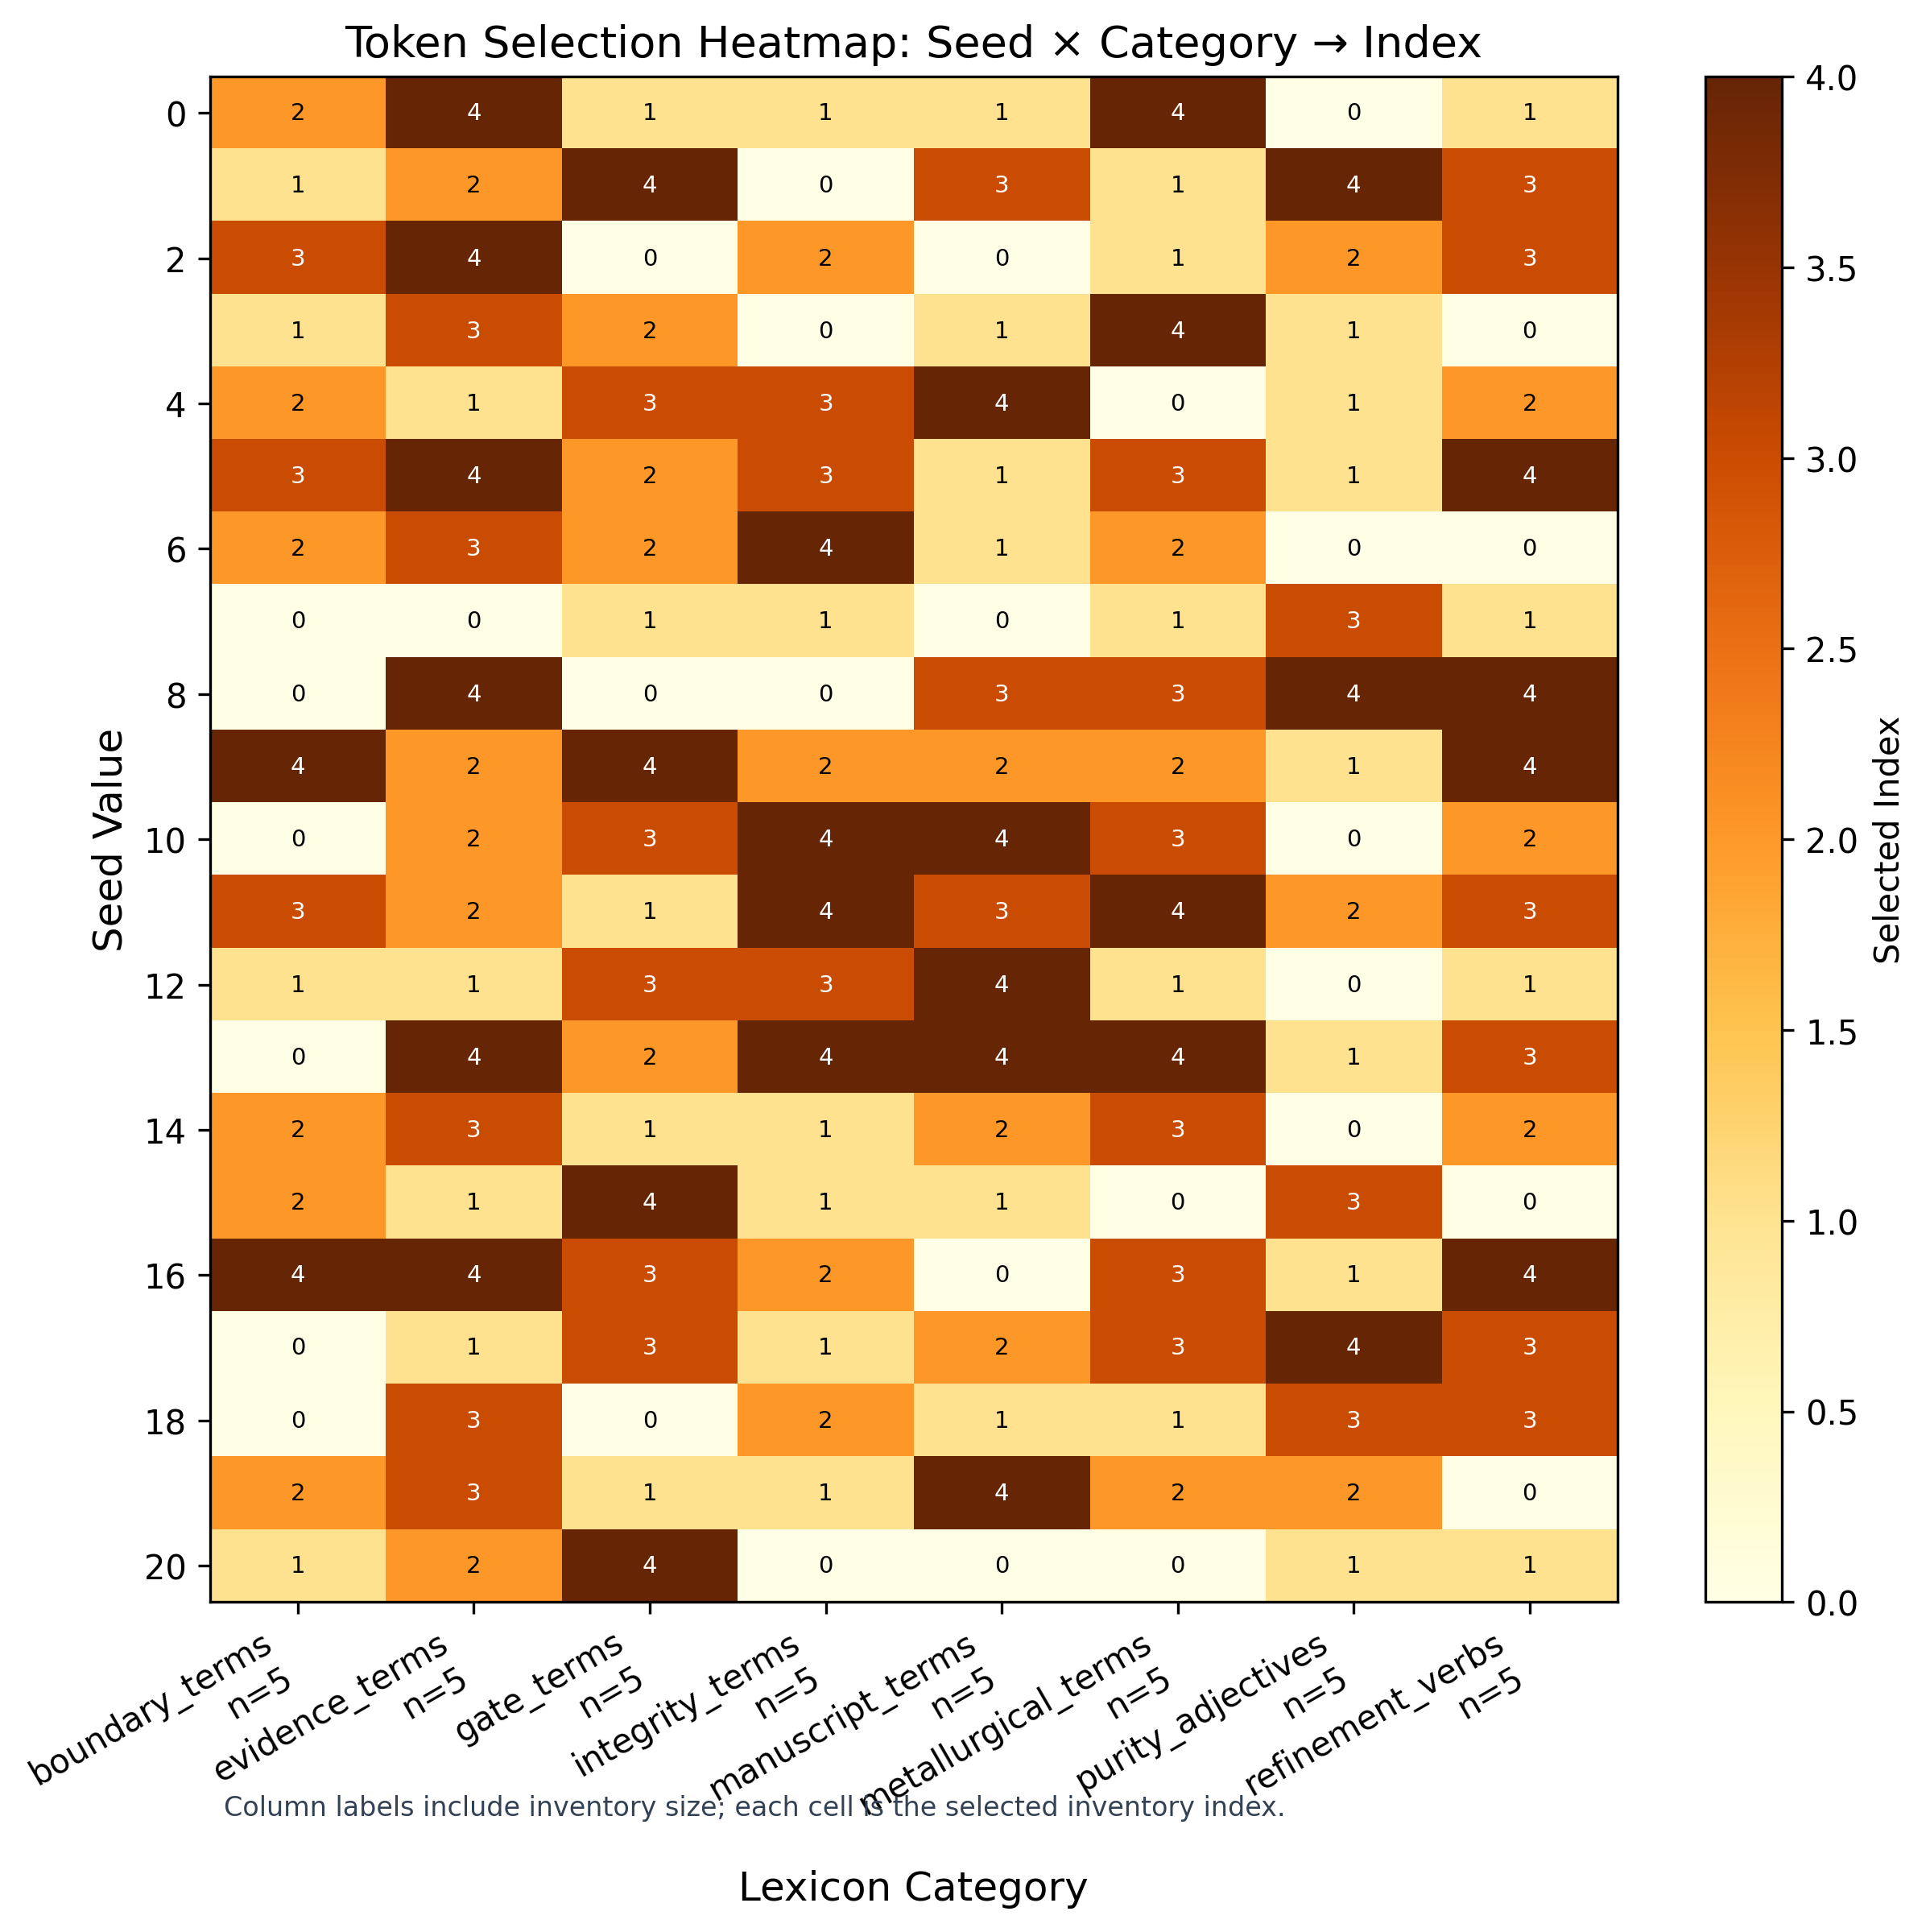
\includegraphics[keepaspectratio,alt={Token selection heatmap: seed \texorpdfstring{\ensuremath{\times}}{x} category \texorpdfstring{\ensuremath{\to}}{->} selected index.}]{../figures/token_heatmap.png}}
\caption{Token selection heatmap: seed \texorpdfstring{\ensuremath{\times}}{x} category \texorpdfstring{\ensuremath{\to}}{->} selected
index.}\label{fig:token_heatmap}
\end{figure}

\subsection{Integrity gate matrix}\label{integrity-gate-matrix}

The integrity gate matrix in fig.~\ref{fig:integrity_gate_matrix} makes
the validation story visible: audit rules are not prose promises unless
they connect to tests, manuscript surfaces, and generated artifacts.

Each row begins as a configured audit rule, but the matrix asks whether
that rule has enough contact with the project to matter. A rule that
names a risk but does not touch tests, manuscript text, or generated
outputs remains advisory. A rule that reaches all three surfaces becomes
enforceable: tests can fail, manuscript hydration can expose stale or
missing variables, and generated reports can show whether the artifact
exists. The matrix is therefore a map of operational coverage, not a
checklist of intentions.

This is the validation story that supports the broader purity analogy.
Smelting can remove obvious dross, but scientific-integrity failures
often survive as well-written unsupported claims, stale tables, or
figures that no longer match their source data. By separating missing,
partial, and full coverage across gate surfaces,
fig.~\ref{fig:integrity_gate_matrix} identifies where a future author
would need to add a test, generated artifact, or manuscript variable
before strengthening a claim. The result is intentionally local to this
exemplar: coverage is measured against the specific audit rules
configured here, not against a universal publication-readiness standard.

\begin{figure}
\centering
\pandocbounded{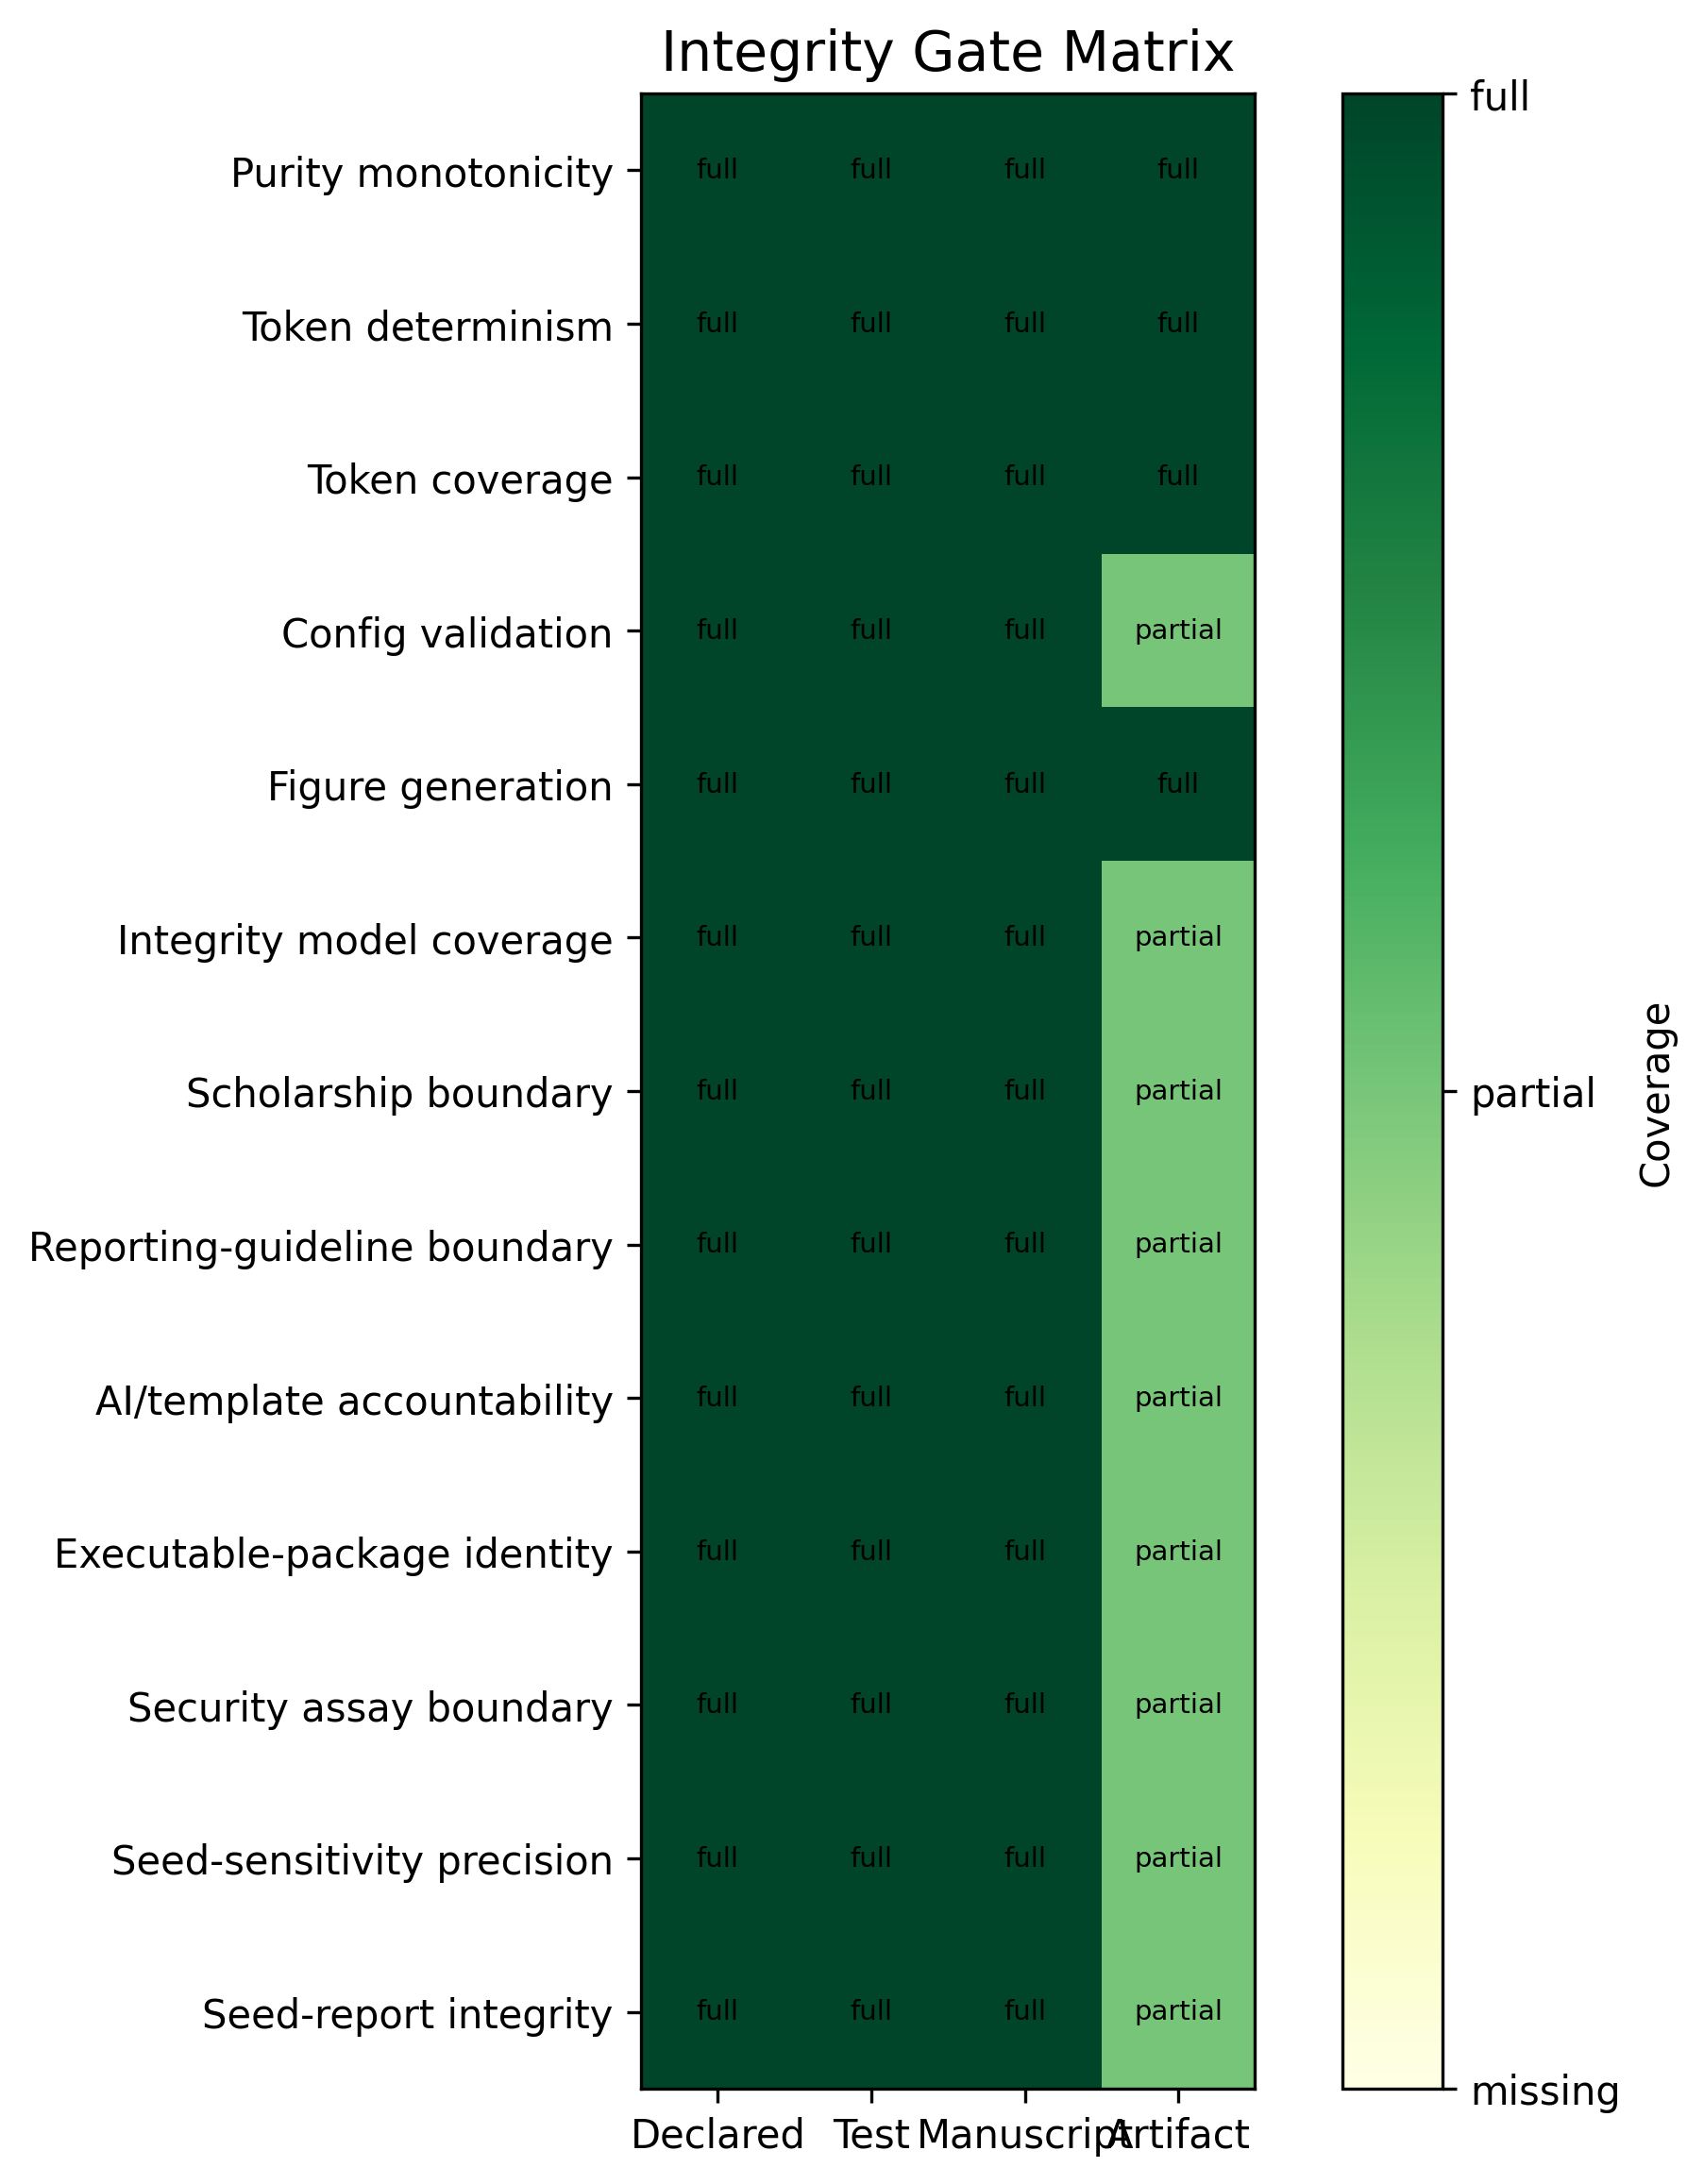
\includegraphics[keepaspectratio,alt={Integrity-gate matrix linking audit rules to tests, manuscript surfaces, and generated artifacts.}]{../figures/integrity_gate_matrix.png}}
\caption{Integrity-gate matrix linking audit rules to tests, manuscript
surfaces, and generated artifacts.}\label{fig:integrity_gate_matrix}
\end{figure}

\subsection{Formalism traceability}\label{formalism-traceability}

The formalism traceability view in fig.~\ref{fig:formalism_traceability}
links each equation-backed formalism to the source surface that owns it.
This is the visual counterpart to tbl.~\ref{tbl:formalism_registry}.

The registry currently exposes 7 source-owned formalisms. The figure
makes their ownership legible by linking each formalism to its equation
identifier and to the source surface that emits it. That linkage is
important because equation labels can otherwise create a false sense of
rigor: a numbered equation looks formal even when its assumptions,
variables, and implementation owner are not recoverable. Here the formal
object must remain connected to \breaktt{src/formalisms.py}, the
generated registry table, and the manuscript reference that consumes it.

The graph also helps distinguish formal support from decorative
notation. A formalism earns a place in the manuscript only when it names
a claim boundary or computation that the source can regenerate. If an
equation is added without a source owner, it should fail this
traceability pattern before it becomes part of the results narrative.
Conversely, if the source registry changes, the visual traceability
layer should change with it. That is the desired behavior: the formal
layer is a generated contract, not hand-maintained mathematical
ornamentation.

\begin{figure}
\centering
\pandocbounded{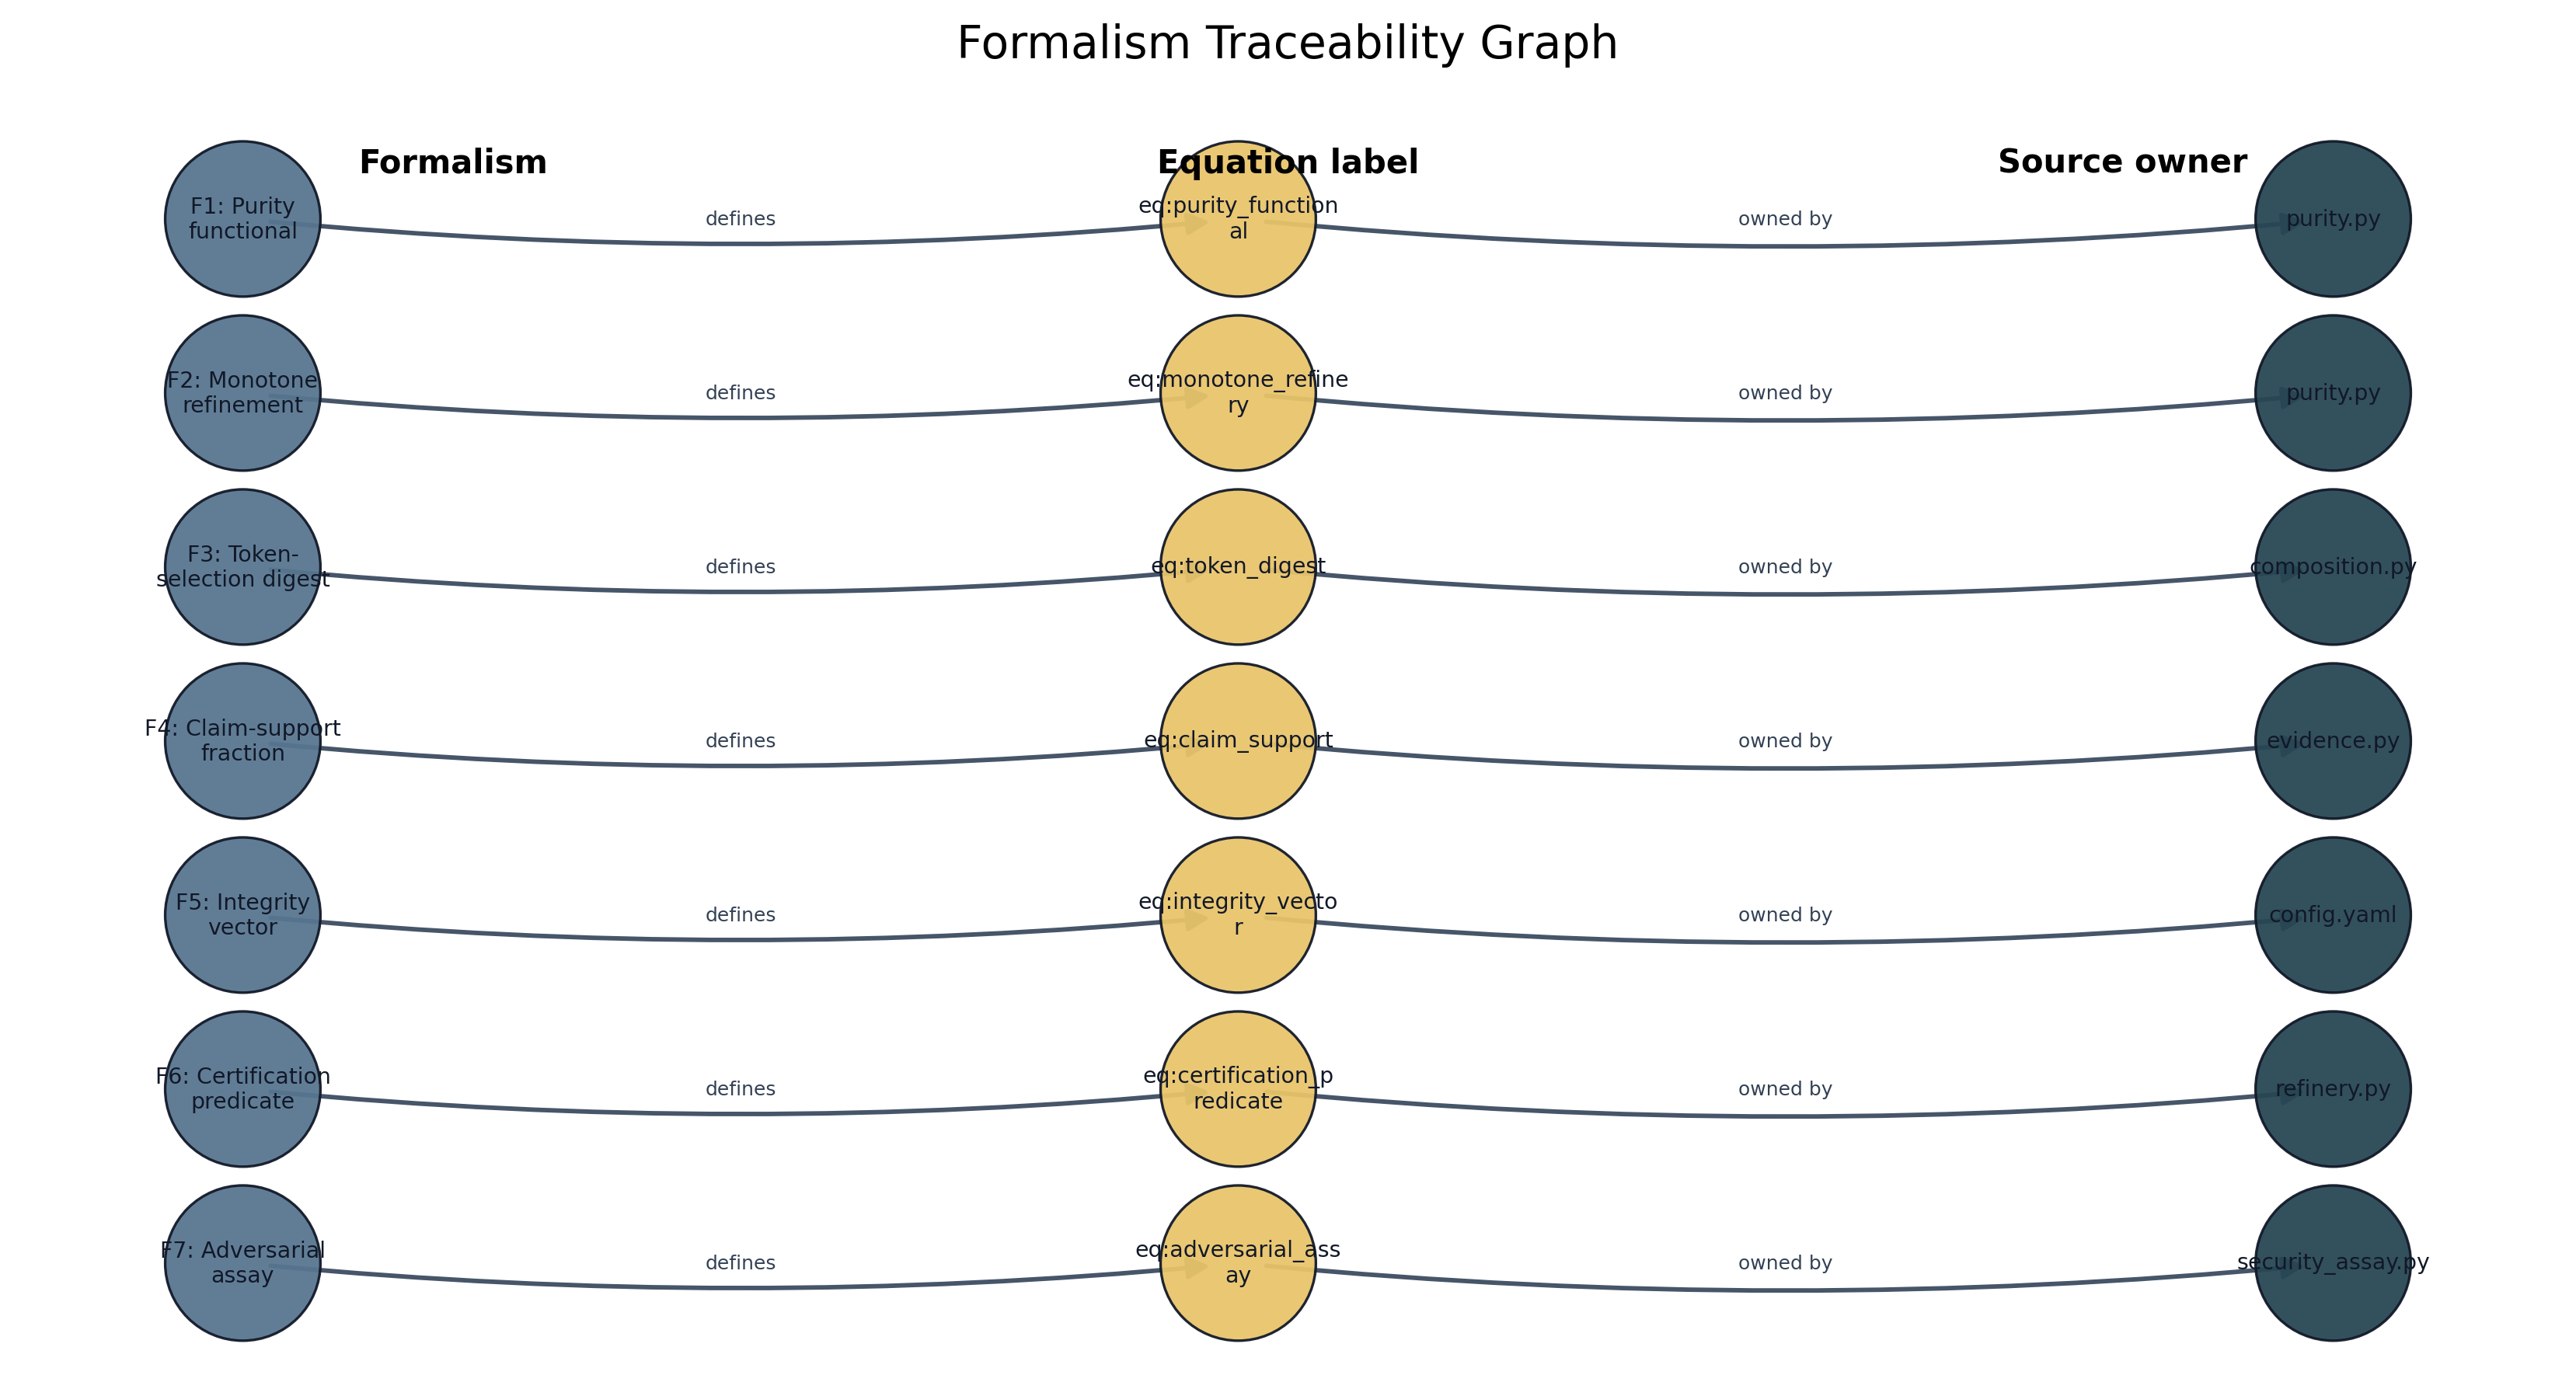
\includegraphics[keepaspectratio,alt={Formalism traceability from source-owned equation identifiers to source evidence.}]{../figures/formalism_traceability.png}}
\caption{Formalism traceability from source-owned equation identifiers
to source evidence.}\label{fig:formalism_traceability}
\end{figure}

\subsection{Implementation circuit}\label{implementation-circuit-1}

The implementation circuit in fig.~\ref{fig:implementation_circuit}
shows how the concept is executed rather than merely described.
Configuration feeds code; code emits variables, figures, and reports;
manuscript hydration consumes those artifacts; validators feed errors
back to source ownership. The figure is intentionally circular because
the artifact is not complete after prose generation. It is complete only
after the validation return path has no blocking evidence, citation,
reference, or render failures.

The circuit is the results section's strongest guard against a
prose-only interpretation of the template. It shows four layers that
must remain connected: configuration, project code, generated artifacts,
and validation feedback. A change in \breaktt{manuscript/config.yaml} is
not complete when the file is saved. It must pass through source
functions, generate updated variables and figures, hydrate the
manuscript, and survive the validator return path. The circular layout
is therefore a process claim: the manuscript is complete only when the
loop closes without unresolved failures.

This view also explains why the exemplar treats generated output as
disposable but not optional. Output files are not edited by hand, yet
they are the evidence surface through which the reader and validators
inspect the source contract. When a validator reports a broken citation,
missing figure, stale variable, or unsupported claim, the circuit points
backward to the owning source surface rather than encouraging local
patching of rendered Markdown. That direction of repair is central to
the manuscript's definition of refinement.

\begin{figure}
\centering
\pandocbounded{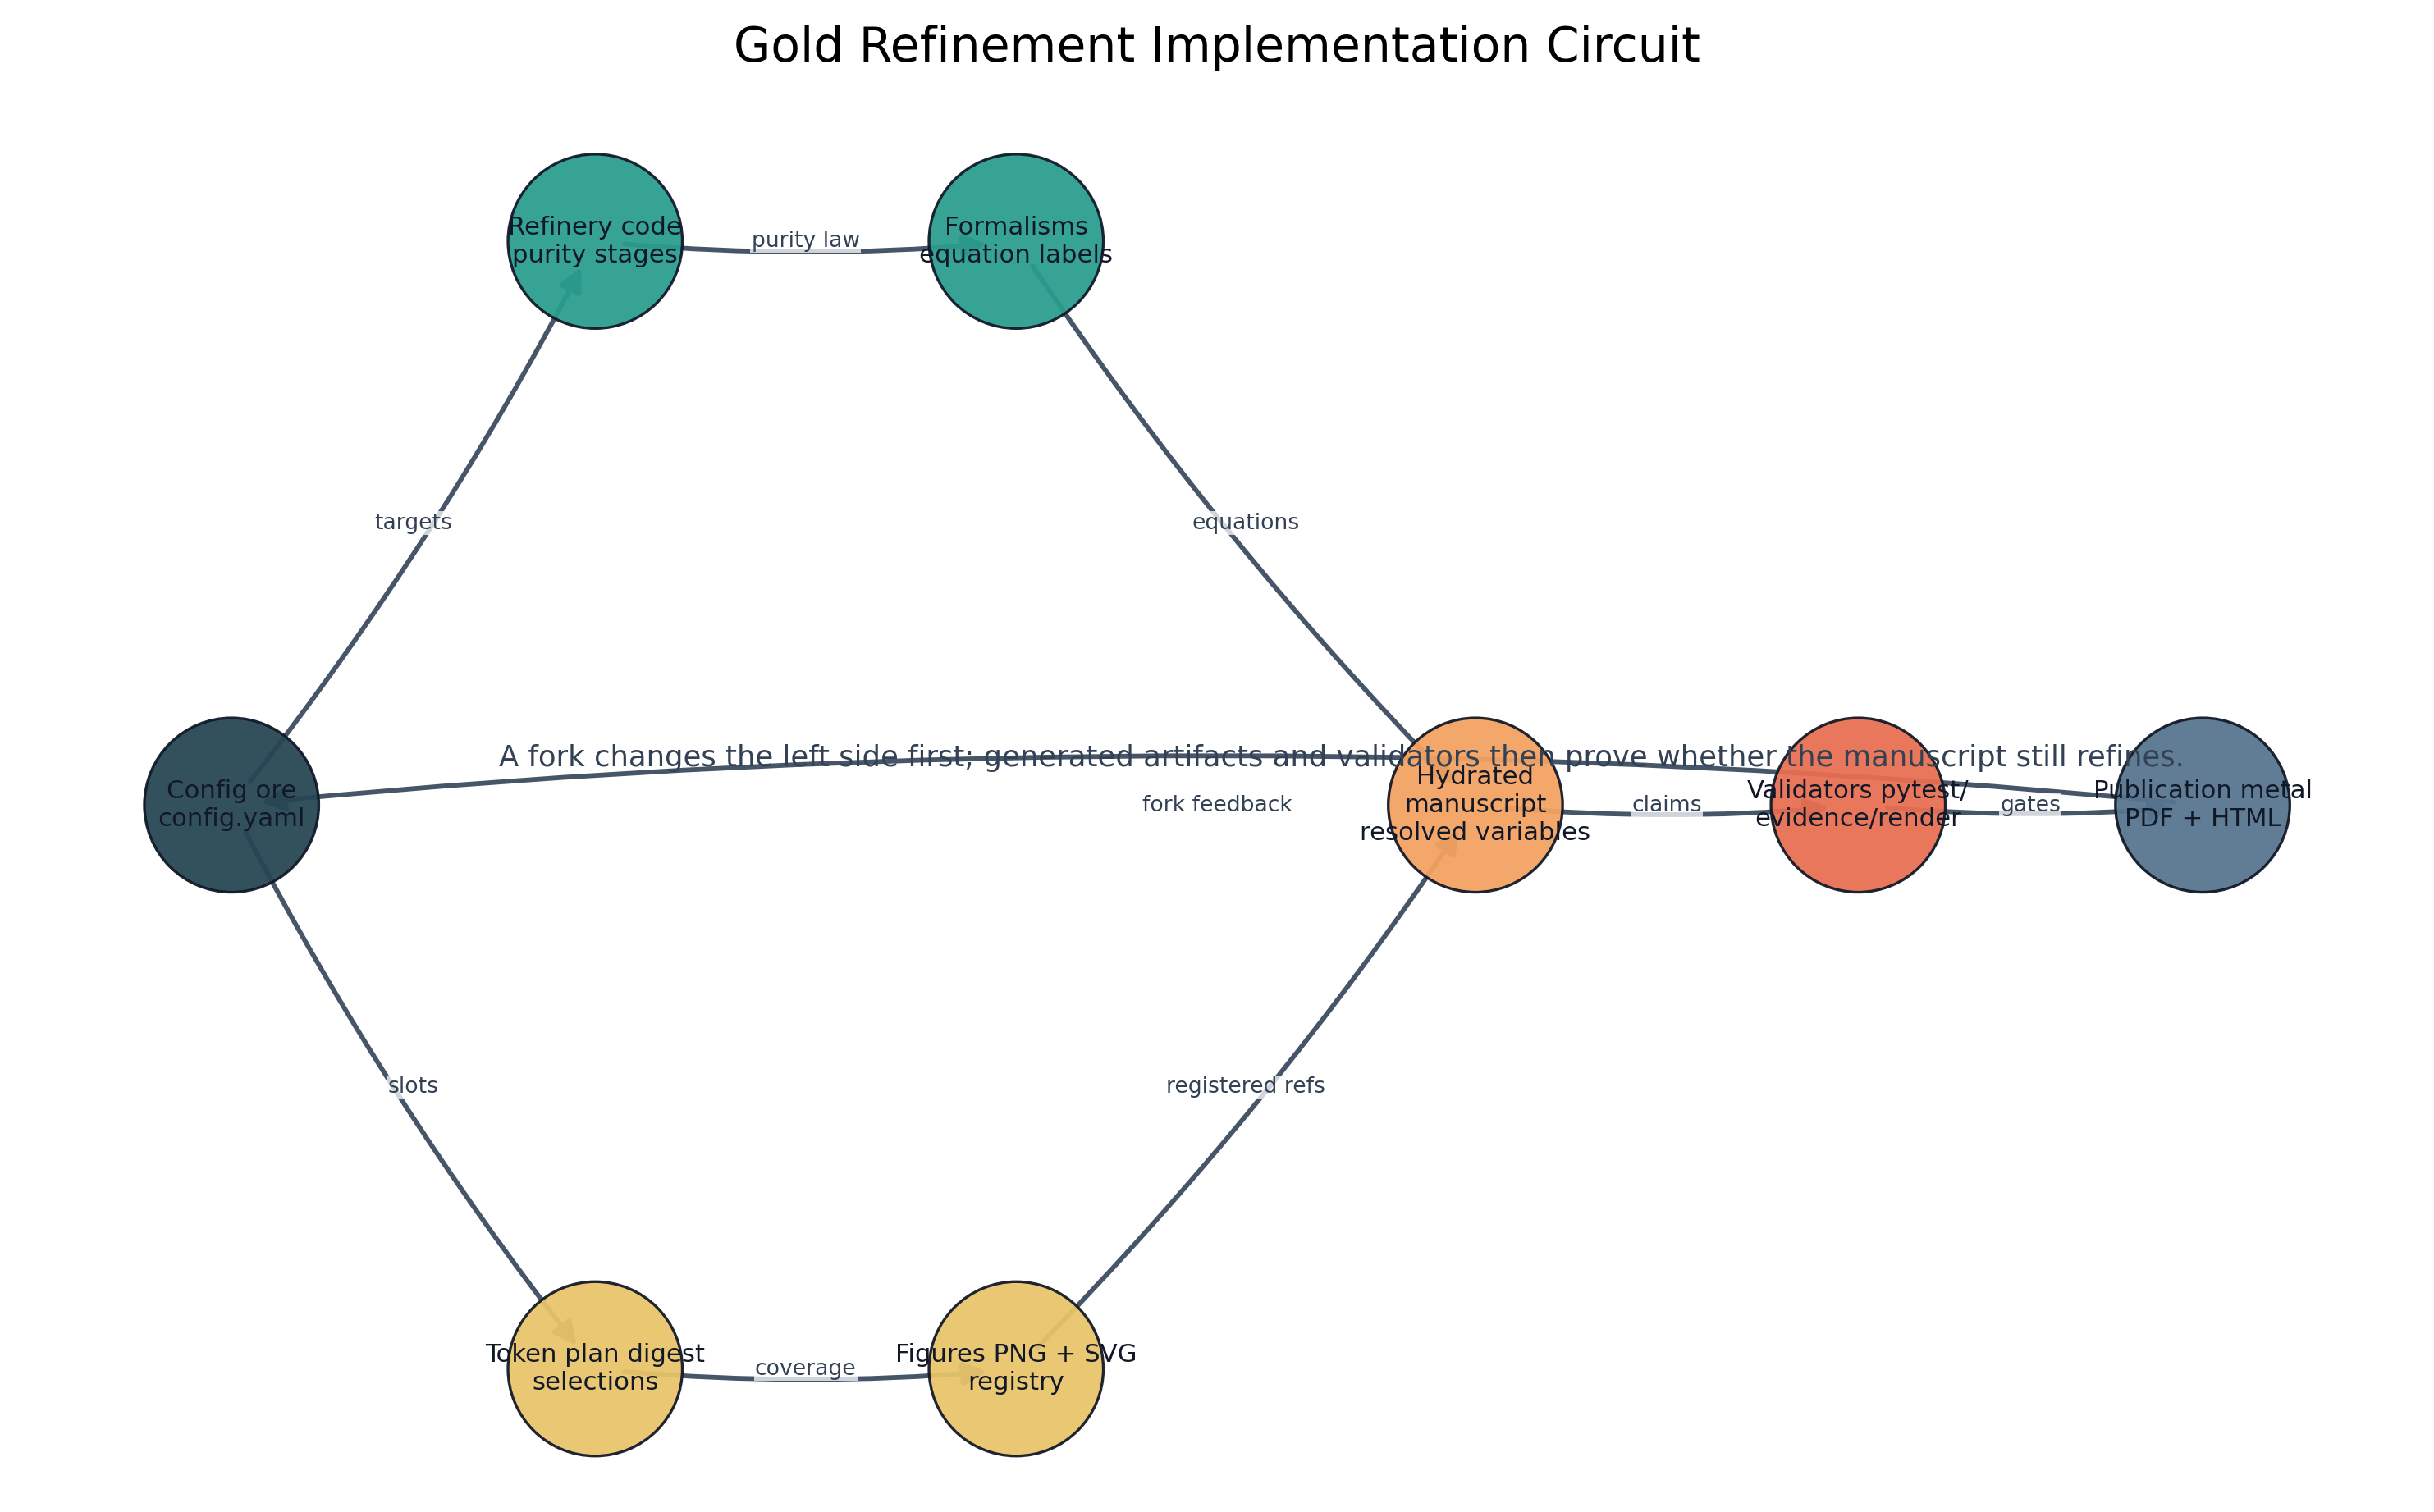
\includegraphics[keepaspectratio,alt={Implementation circuit from config-owned ore through generated manuscript artifacts and validation feedback.}]{../figures/implementation_circuit.png}}
\caption{Implementation circuit from config-owned ore through generated
manuscript artifacts and validation
feedback.}\label{fig:implementation_circuit}
\end{figure}

\subsection{Claim-evidence assay}\label{claim-evidence-assay}

The claim-evidence assay in fig.~\ref{fig:claim_evidence_assay} turns
the assaying stage into a reader-facing diagnostic. Each bar is a
contribution claim from \breaktt{manuscript/config.yaml}, and each
annotation names the source file or symbol used to support it. This
makes the contribution ledger inspectable at the same level as the
purity plots: unsupported claims would appear as failed assays rather
than remaining hidden in prose.

The generated assay currently reports 10 supported claims out of 10. The
value of the figure is not the perfect score by itself; it is the way
the score is forced to name its evidence surface and boundary. A
contribution claim is not merely present in prose. It must be
registered, matched to supporting evidence, and assigned a boundary that
tells the reader what the support does not cover. This keeps
contribution language from drifting beyond the local evidence available
in the project.

The bar-plus-topology design makes two failure modes visible. If a claim
lacks support, the bar view would show the failed assay directly. If a
claim is supported only within a narrow scope, the graph side still
preserves the boundary classification rather than flattening the result
into a binary pass. That matters for the security and integrity
extensions in this manuscript: a claim can be source-owned without
becoming a compliance claim, and a generated assay can confirm local
evidence without pretending to certify the wider supply chain.

\begin{figure}
\centering
\pandocbounded{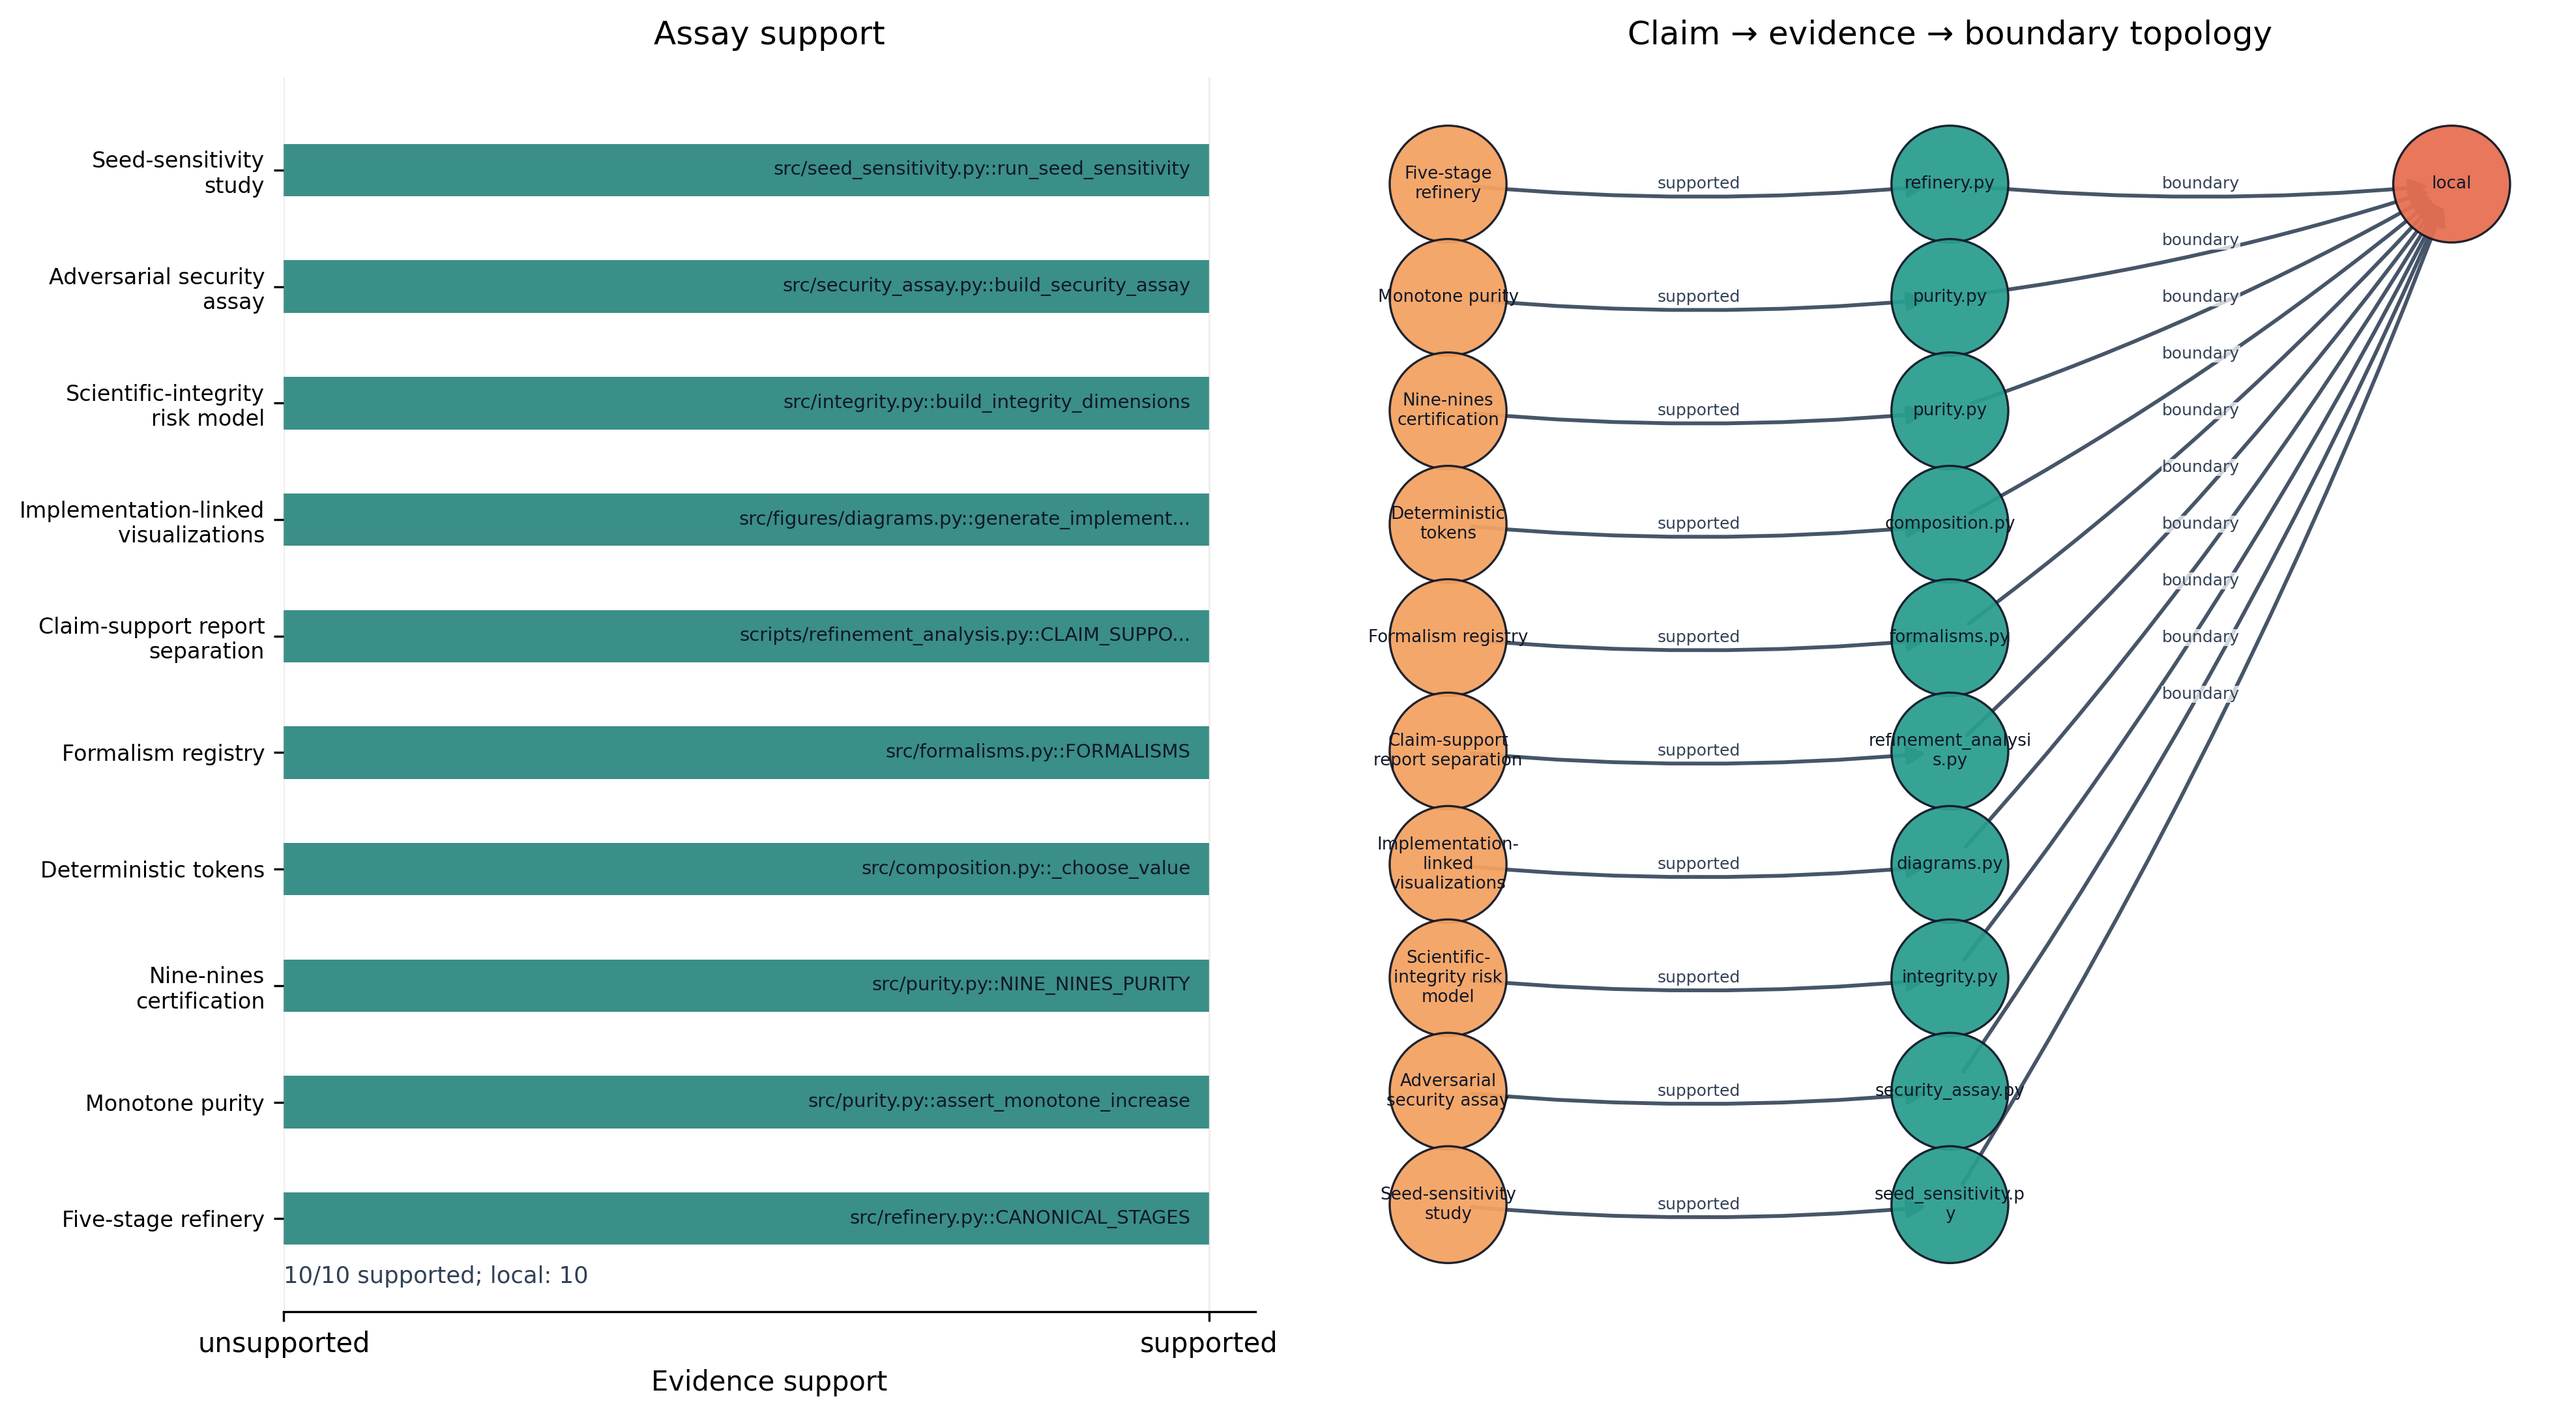
\includegraphics[keepaspectratio,alt={Claim-evidence assay showing supported contribution claims, evidence surfaces, and boundary classifications.}]{../figures/claim_evidence_assay.png}}
\caption{Claim-evidence assay showing supported contribution claims,
evidence surfaces, and boundary
classifications.}\label{fig:claim_evidence_assay}
\end{figure}

\subsection{Scientific-integrity risk
matrix}\label{scientific-integrity-risk-matrix}

The integrity risk matrix in fig.~\ref{fig:integrity_risk_matrix} plots
severity against detectability for the 9 integrity dimensions in
tbl.~\ref{tbl:integrity_dimensions}. Bubble size encodes residual risk,
while color encodes the source tier that owns the evidence surface. This
makes boundary failures more visible than cosmetic source checks without
hiding whether the support comes from config, source code, claim ledger,
generated metric, artifact, bibliography, or validation gate. The matrix
is intentionally local: it prioritizes where this exemplar needs source
ownership, not where every future manuscript should focus.

The generated summary is: 9 integrity dimensions; highest residual risk
is I4 (Analogy boundary) at 15. The matrix turns that summary into a
triage surface. Severity asks how damaging a failure would be if it
entered the manuscript. Detectability asks how readily the current
project would catch it. Residual risk then becomes visible as size
rather than being buried in a paragraph. A large point in a
hard-to-detect region is a signal that the authoring contract needs
stronger source ownership or a clearer boundary, even if the current
text renders successfully.

Color is equally important because not all evidence tiers have the same
authority. A bibliography-backed statement, a source-code computation, a
claim ledger row, and a validation-gate result can all support prose,
but they support different kinds of claims. The risk matrix keeps that
distinction visible. It does not collapse integrity into a single score,
and it does not imply that every high-severity issue has already been
eliminated. It shows which risks this exemplar has made inspectable and
where future work would need to add stronger measurement before using
stronger language.

\begin{figure}
\centering
\pandocbounded{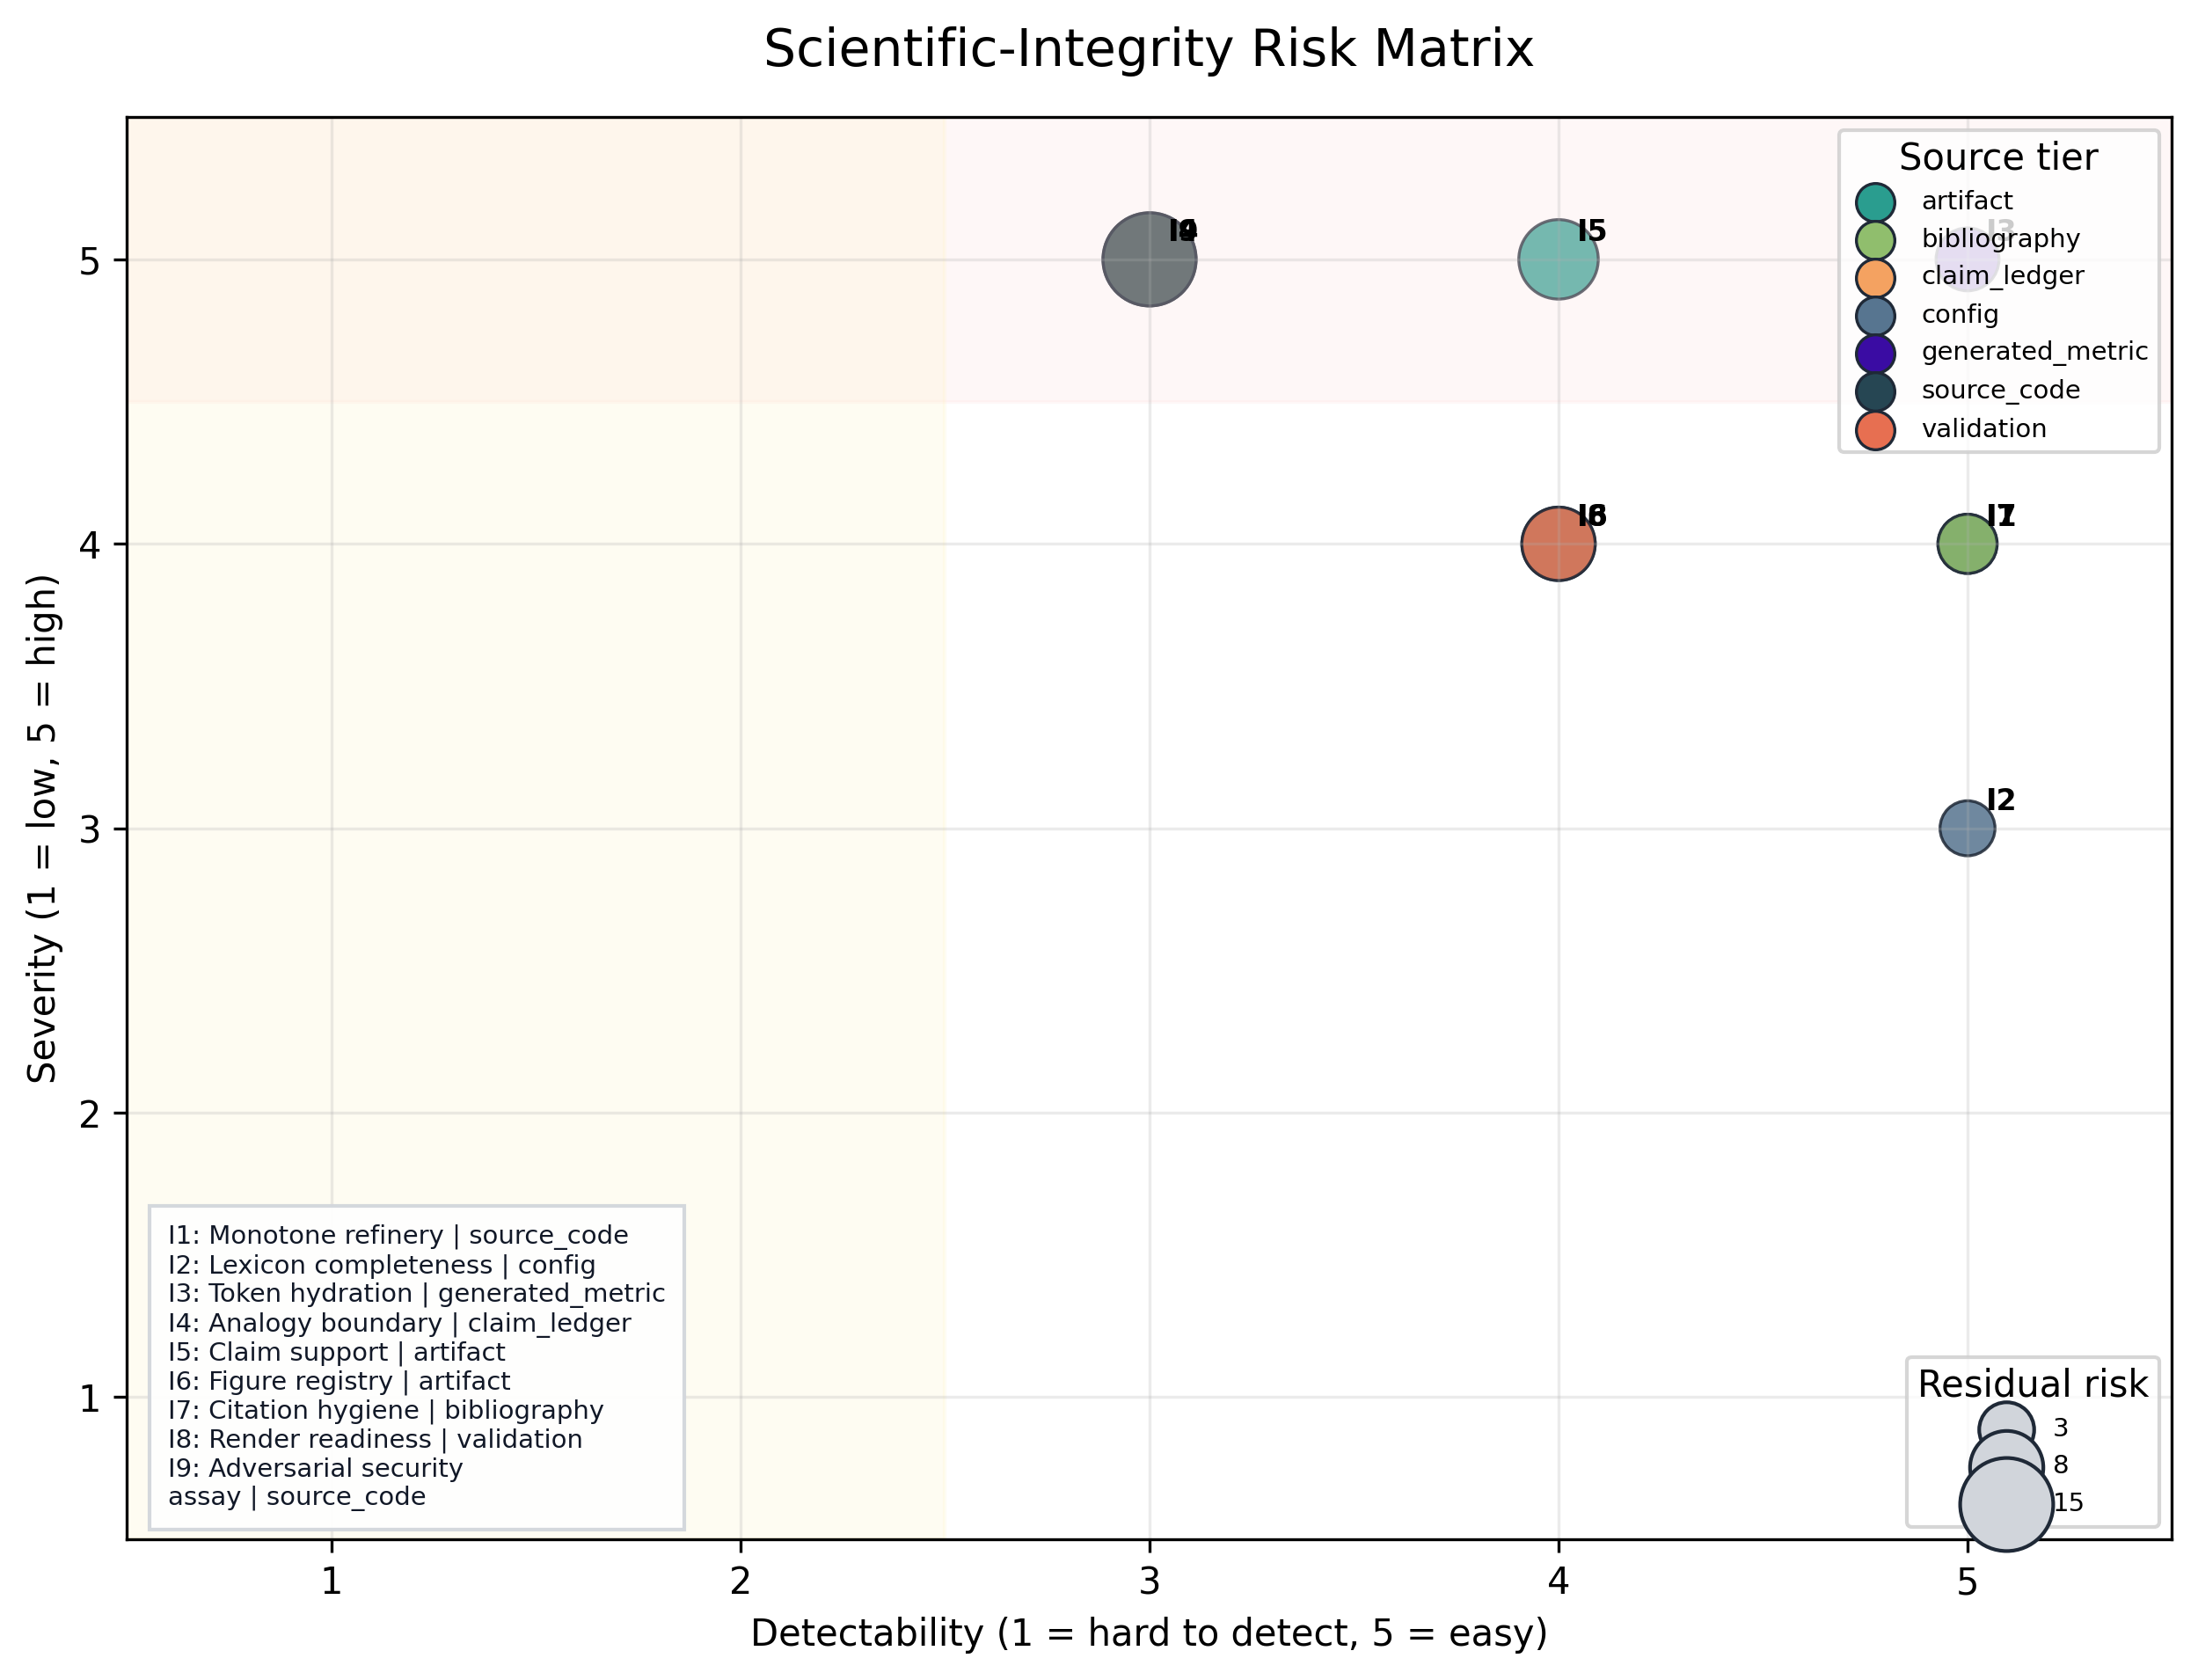
\includegraphics[keepaspectratio,alt={Scientific-integrity risk matrix plotting severity, detectability, residual risk, and owning evidence surface.}]{../figures/integrity_risk_matrix.png}}
\caption{Scientific-integrity risk matrix plotting severity,
detectability, residual risk, and owning evidence
surface.}\label{fig:integrity_risk_matrix}
\end{figure}

\subsection{Evidence-tier ladder}\label{evidence-tier-ladder}

The evidence-tier ladder in fig.~\ref{fig:evidence_tier_ladder}
summarizes the evidence surfaces available to the shared template
evidence registry or, before that gate has run, the fallback source
tiers from the integrity model. It gives a quick view of whether the
manuscript is leaning on generated metrics, claim-ledger facts,
bibliography records, source code, or disposable artifacts.

The ladder complements the risk matrix by counting source tiers rather
than plotting risks. When the shared evidence registry is available, the
manuscript can report 15577 source-tiered facts to the validation
surface. When that registry is not available, the same figure falls back
to the integrity model's configured tiers. Either way, the reader sees
the evidentiary mix instead of receiving an undifferentiated assurance
that evidence exists.

This matters because evidence balance is itself an integrity signal. A
manuscript that leans only on generated artifacts may be reproducible
but weakly grounded in source rationale. A manuscript that leans only on
bibliography may be well-cited but not locally executable. A manuscript
that leans only on tests may catch regressions while still failing to
explain claim boundaries to readers. The ladder gives a compact audit of
that mix, while tbl.~\ref{tbl:evidence_tiers} keeps the counts visible
in tabular form. Together they close the figure sequence by showing not
only that the 13 public figures render, but also which source tiers make
their claims inspectable.

\begin{figure}
\centering
\pandocbounded{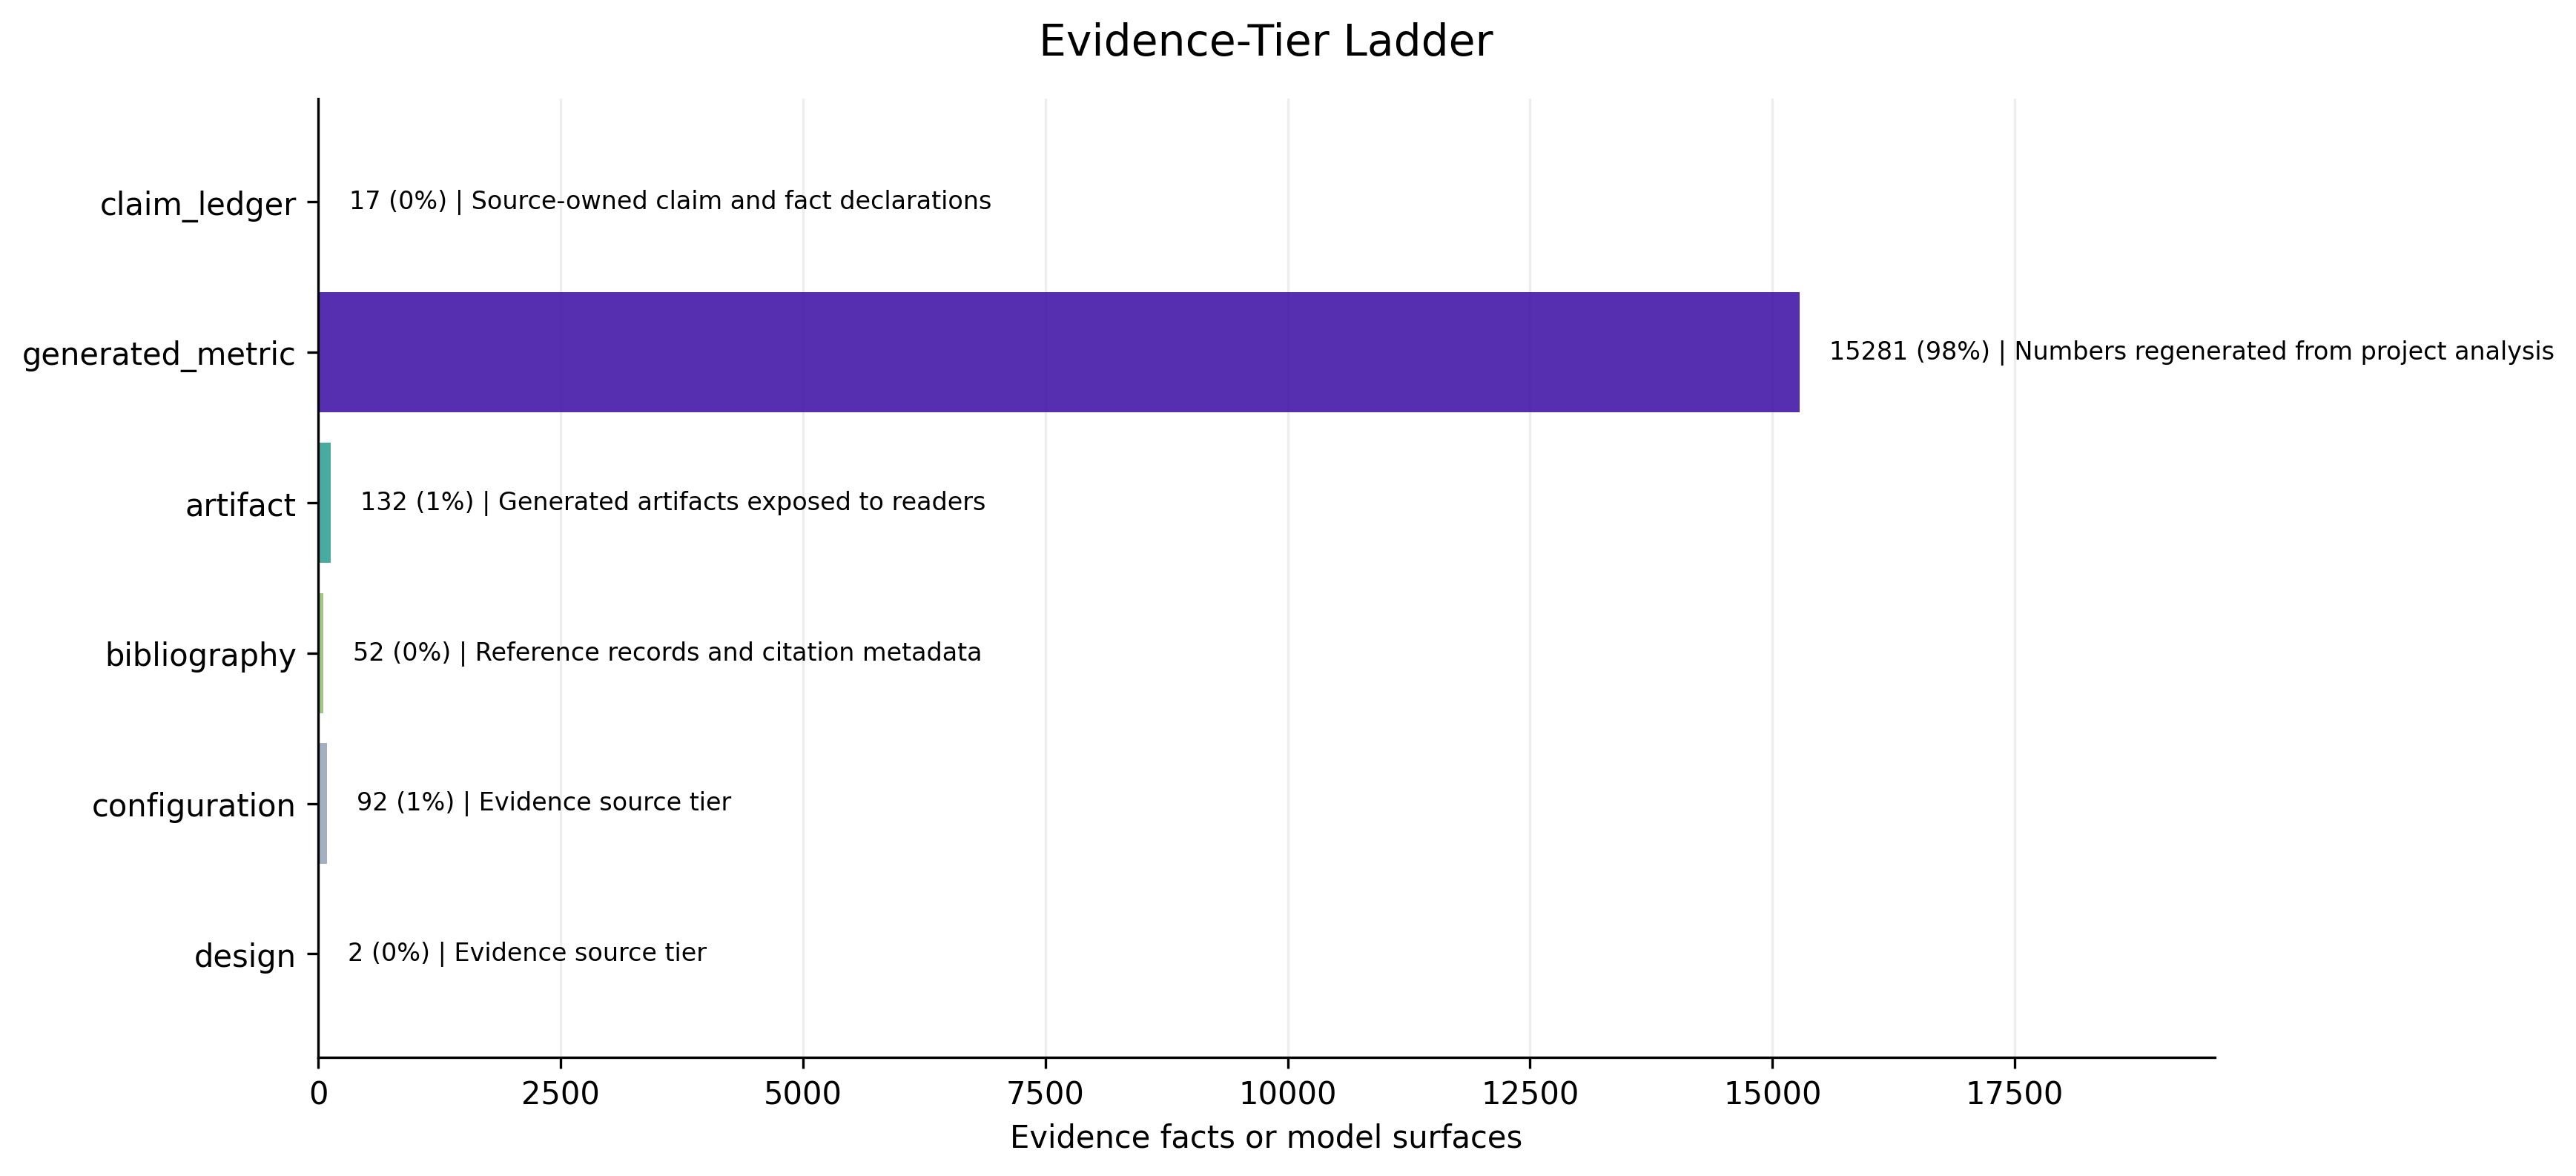
\includegraphics[keepaspectratio,alt={Evidence-tier ladder summarizing source tiers available to the shared template evidence registry.}]{../figures/evidence_tier_ladder.png}}
\caption{Evidence-tier ladder summarizing source tiers available to the
shared template evidence registry.}\label{fig:evidence_tier_ladder}
\end{figure}

\begin{longtable}[]{@{}lll@{}}
\caption{Evidence tiers used by the integrity model and shared registry
when available.}\label{tbl:evidence_tiers}\tabularnewline
\toprule\noalign{}
Source tier & Count & Role \\
\midrule\noalign{}
\endfirsthead
\toprule\noalign{}
Source tier & Count & Role \\
\midrule\noalign{}
\endhead
\bottomrule\noalign{}
\endlastfoot
generated\_metric & 15282 & Numbers regenerated from project analysis \\
artifact & 132 & Generated artifacts exposed to readers \\
configuration & 92 & Evidence source tier \\
bibliography & 52 & Reference records and citation metadata \\
claim\_ledger & 17 & Source-owned claim and fact declarations \\
design & 2 & Evidence source tier \\
\end{longtable}

\subsection{Adversarial security
assay}\label{adversarial-security-assay}

The adversarial assay reports 5 adversarial assay rows, 5
schema-complete, mapping threats and standards to local evidence
surfaces, validators, and claim boundaries; completeness is a scope
control, not completed scan findings. No Codex Security or Deep Security
Scan findings are claimed unless a scan artifact is generated,
validated, and cited. The rows are generated from
\breaktt{gold\_refinement.security\_assay} and are intentionally tabular
rather than a new public figure, so the visual registry remains the
stable 13-figure contract.

\begin{longtable}[]{@{}
  >{\raggedright\arraybackslash}p{(\linewidth - 10\tabcolsep) * \real{0.0460}}
  >{\raggedright\arraybackslash}p{(\linewidth - 10\tabcolsep) * \real{0.0920}}
  >{\raggedright\arraybackslash}p{(\linewidth - 10\tabcolsep) * \real{0.2529}}
  >{\raggedright\arraybackslash}p{(\linewidth - 10\tabcolsep) * \real{0.2069}}
  >{\raggedright\arraybackslash}p{(\linewidth - 10\tabcolsep) * \real{0.2184}}
  >{\raggedright\arraybackslash}p{(\linewidth - 10\tabcolsep) * \real{0.1839}}@{}}
\caption{Source-owned adversarial security
assay.}\label{tbl:security_assay}\tabularnewline
\toprule\noalign{}
\begin{minipage}[b]{\linewidth}\raggedright
ID
\end{minipage} & \begin{minipage}[b]{\linewidth}\raggedright
Threat
\end{minipage} & \begin{minipage}[b]{\linewidth}\raggedright
Standard or guidance
\end{minipage} & \begin{minipage}[b]{\linewidth}\raggedright
Evidence surface
\end{minipage} & \begin{minipage}[b]{\linewidth}\raggedright
Validator or gate
\end{minipage} & \begin{minipage}[b]{\linewidth}\raggedright
Claim boundary
\end{minipage} \\
\midrule\noalign{}
\endfirsthead
\toprule\noalign{}
\begin{minipage}[b]{\linewidth}\raggedright
ID
\end{minipage} & \begin{minipage}[b]{\linewidth}\raggedright
Threat
\end{minipage} & \begin{minipage}[b]{\linewidth}\raggedright
Standard or guidance
\end{minipage} & \begin{minipage}[b]{\linewidth}\raggedright
Evidence surface
\end{minipage} & \begin{minipage}[b]{\linewidth}\raggedright
Validator or gate
\end{minipage} & \begin{minipage}[b]{\linewidth}\raggedright
Claim boundary
\end{minipage} \\
\midrule\noalign{}
\endhead
\bottomrule\noalign{}
\endlastfoot
S1 & implicit trust in generated artifacts & NIST SP 800-207 zero trust
& output/reports/evidence\_registry.json and src/security\_assay.py &
infrastructure.validation.cli evidence --fail-on-issues & documents a
verification posture, not a deployed zero-trust architecture \\
S2 & incomplete secure-development evidence & NIST SP 800-218 secure
software development framework & tests/, pre-render validation, and
claim ledger & project test suite and template validation gates & maps
local practices to SSDF concepts without claiming SSDF compliance \\
S3 & supply-chain or build provenance compromise & SLSA v1.2, Sigstore,
SPDX, and CycloneDX & config hash, artifact counts, and publication
metadata & pipeline regeneration and artifact registry checks &
identifies provenance requirements but does not assert signed SBOM or
provenance is present \\
S4 & unvalidated vulnerability narrative & MITRE ATT\&CK and Codex
Security scan phases & security assay table and future scan artifacts &
Codex Security threat-model, discovery, validation, and attack-path
receipts when run & no real scan finding is claimed in this manuscript
pass \\
S5 & secure-by-design overclaim & CISA Secure by Design & authoring
contract and scope limitations & human source review plus citation and
evidence validation & uses guidance to bound responsibilities, not to
certify product security \\
\end{longtable}

\subsection{Contribution claims}\label{contribution-claims}

{\def\LTcaptype{none} % do not increment counter
\begin{longtable}[]{@{}
  >{\raggedright\arraybackslash}p{(\linewidth - 6\tabcolsep) * \real{0.1842}}
  >{\raggedright\arraybackslash}p{(\linewidth - 6\tabcolsep) * \real{0.2895}}
  >{\raggedright\arraybackslash}p{(\linewidth - 6\tabcolsep) * \real{0.2632}}
  >{\raggedright\arraybackslash}p{(\linewidth - 6\tabcolsep) * \real{0.2632}}@{}}
\toprule\noalign{}
\begin{minipage}[b]{\linewidth}\raggedright
Claim
\end{minipage} & \begin{minipage}[b]{\linewidth}\raggedright
Statement
\end{minipage} & \begin{minipage}[b]{\linewidth}\raggedright
Evidence
\end{minipage} & \begin{minipage}[b]{\linewidth}\raggedright
Boundary
\end{minipage} \\
\midrule\noalign{}
\endhead
\bottomrule\noalign{}
\endlastfoot
Five-stage refinery & The refinery pipeline has 5 canonical stages from
ore to nine-nines. & src/refinery.py::CANONICAL\_STAGES & local \\
Monotone purity & Purity increases strictly across all refinery stages.
& src/purity.py::assert\_monotone\_increase & local \\
Nine-nines certification & The certification stage achieves 99.9999999\%
purity. & src/purity.py::NINE\_NINES\_PURITY & local \\
Deterministic tokens & Token selection is deterministic via seeded
SHA-256 digest. & src/composition.py::\_choose\_value & local \\
Formalism registry & The manuscript exposes 7 source-owned formalisms
with equation labels. & src/formalisms.py::FORMALISMS & local \\
Claim-support report separation & The project-local contribution-claim
report is written to claim\_support\_registry.json. &
scripts/refinement\_analysis.py::CLAIM\_SUPPORT\_REGISTRY\_NAME &
local \\
Implementation-linked visualizations & The manuscript includes generated
visualizations that link the refinery analogy to source code, variables,
evidence, and validation gates. &
src/figures/diagrams.py::generate\_implementation\_circuit & local \\
Scientific-integrity risk model & The manuscript includes a source-owned
integrity risk model linking failure modes, validators, evidence
surfaces, and fork obligations. &
src/integrity.py::build\_integrity\_dimensions & local \\
Adversarial security assay & The manuscript includes a source-owned
security assay mapping adversarial threats and standards to local
evidence surfaces, validators, and claim boundaries. &
src/security\_assay.py::build\_security\_assay & local \\
Seed-sensitivity study & The project reports a declared seed-replicate
sensitivity study with precision metadata and explicit non-empirical
boundaries. & src/seed\_sensitivity.py::run\_seed\_sensitivity &
local \\
\end{longtable}
}

The project-local claim-support assay reports 10 supported claims out of
10 total claims, for 100.00\% support. Unsupported claims: 0. The
generated project report path is
\breaktt{output/reports/claim\_support\_registry.json}; the shared
template evidence report remains
\breaktt{output/reports/evidence\_registry.json}.

\subsection{Shared evidence registry
summary}\label{shared-evidence-registry-summary}

When the template evidence gate has run, the shared registry supplies
source-tiered facts used by the evidence validator. Current fact count
available to this variable pass: 15577.

\begin{longtable}[]{@{}ll@{}}
\caption{Shared evidence-registry fact kinds when
available.}\label{tbl:shared_evidence_kinds}\tabularnewline
\toprule\noalign{}
Fact kind & Count \\
\midrule\noalign{}
\endfirsthead
\toprule\noalign{}
Fact kind & Count \\
\midrule\noalign{}
\endhead
\bottomrule\noalign{}
\endlastfoot
artifact & 84 \\
citation & 52 \\
equation & 8 \\
figure & 31 \\
number & 15384 \\
section & 10 \\
table & 8 \\
\end{longtable}

\subsection{Figure quality report}\label{figure-quality-report}

The visualization registry is paired with
\breaktt{output/reports/figure\_quality\_report.json}, a generated QA
report that checks PNG and SVG existence, file dimensions, nonblank
pixel mass, color variance, and registry parity. Current status: passing
with 13/13 registered figures passing and registry parity reported as
Yes. PNG remains the manuscript render path; SVG is the companion
technical artifact for inspection, reuse, and source-level debugging.
tbl.~\ref{tbl:figure_quality} summarizes the generated surface.

\begin{longtable}[]{@{}
  >{\raggedright\arraybackslash}p{(\linewidth - 12\tabcolsep) * \real{0.1379}}
  >{\raggedright\arraybackslash}p{(\linewidth - 12\tabcolsep) * \real{0.0862}}
  >{\raggedright\arraybackslash}p{(\linewidth - 12\tabcolsep) * \real{0.0862}}
  >{\raggedright\arraybackslash}p{(\linewidth - 12\tabcolsep) * \real{0.2069}}
  >{\raggedright\arraybackslash}p{(\linewidth - 12\tabcolsep) * \real{0.1724}}
  >{\raggedright\arraybackslash}p{(\linewidth - 12\tabcolsep) * \real{0.1724}}
  >{\raggedright\arraybackslash}p{(\linewidth - 12\tabcolsep) * \real{0.1379}}@{}}
\caption{Figure-quality report generated from source-owned figure
specs.}\label{tbl:figure_quality}\tabularnewline
\toprule\noalign{}
\begin{minipage}[b]{\linewidth}\raggedright
Figure
\end{minipage} & \begin{minipage}[b]{\linewidth}\raggedright
PNG
\end{minipage} & \begin{minipage}[b]{\linewidth}\raggedright
SVG
\end{minipage} & \begin{minipage}[b]{\linewidth}\raggedright
Dimensions
\end{minipage} & \begin{minipage}[b]{\linewidth}\raggedright
Nonwhite
\end{minipage} & \begin{minipage}[b]{\linewidth}\raggedright
Variance
\end{minipage} & \begin{minipage}[b]{\linewidth}\raggedright
Status
\end{minipage} \\
\midrule\noalign{}
\endfirsthead
\toprule\noalign{}
\begin{minipage}[b]{\linewidth}\raggedright
Figure
\end{minipage} & \begin{minipage}[b]{\linewidth}\raggedright
PNG
\end{minipage} & \begin{minipage}[b]{\linewidth}\raggedright
SVG
\end{minipage} & \begin{minipage}[b]{\linewidth}\raggedright
Dimensions
\end{minipage} & \begin{minipage}[b]{\linewidth}\raggedright
Nonwhite
\end{minipage} & \begin{minipage}[b]{\linewidth}\raggedright
Variance
\end{minipage} & \begin{minipage}[b]{\linewidth}\raggedright
Status
\end{minipage} \\
\midrule\noalign{}
\endhead
\bottomrule\noalign{}
\endlastfoot
claim\_evidence\_assay & yes & yes & 3947x2172 & 0.222 & 0.06124546 &
pass \\
evidence\_tier\_ladder & yes & yes & 3463x1586 & 0.083 & 0.03388905 &
pass \\
formalism\_traceability & yes & yes & 3315x1797 & 0.140 & 0.04409869 &
pass \\
implementation\_circuit & yes & yes & 2966x1842 & 0.068 & 0.02214905 &
pass \\
integrity\_gate\_matrix & yes & yes & 1820x2314 & 0.407 & 0.15927030 &
pass \\
integrity\_risk\_matrix & yes & yes & 2499x1909 & 0.379 & 0.01892053 &
pass \\
karat\_grading & yes & yes & 2956x1699 & 0.279 & 0.07296687 & pass \\
provenance\_sankey & yes & yes & 2850x1461 & 0.070 & 0.02170098 &
pass \\
purity\_claim\_scatter & yes & yes & 2343x1745 & 0.034 & 0.01594966 &
pass \\
purity\_progression & yes & yes & 3029x2125 & 0.182 & 0.03971092 &
pass \\
seed\_sensitivity & yes & yes & 3290x1773 & 0.091 & 0.03345077 & pass \\
token\_density & yes & yes & 3288x1858 & 0.234 & 0.06696808 & pass \\
token\_heatmap & yes & yes & 2406x2412 & 0.621 & 0.12867696 & pass \\
\end{longtable}

\newpage

\section{Discussion: Load-Bearing vs Rhetorical
Analogy}\label{sec:discussion}

\subsection{Load-bearing vs
rhetorical}\label{load-bearing-vs-rhetorical}

The gold-refining analogy operates on two levels. \textbf{Rhetorically},
it provides a memorable framing for a methods paper: purity progression,
karat grading, and certification are vivid metaphors for manuscript
quality. \textbf{Operationally}, each stage maps to a real
template-infrastructure operation - smelting to claim removal, assaying
to evidence validation, cupellation to cross-reference resolution, and
certification to full pipeline validation. The scholarship makes the
test sharper: the analogy is useful only where the relation among stages
is preserved, not where surface language makes writing sound like
metallurgy \citep{gentner1983structure, hesse1966models}.

The pre-1800 metallurgy sources strengthen the analogy by making that
relation historically concrete, but they also narrow it. They show
several traditions of staged work - ancient extraction and testing,
Renaissance printed metallurgy, seventeenth-century goldsmith standards,
and eighteenth-century assay manuals - rather than one timeless method
\citep{pliny_natural_history_33, biringuccio_pirotechnia_1540, agricola_de_re_metallica_1556, badcock_touchstone_1678, cramer_assaying_metals_1741}.
The manuscript therefore imports structure, not authority: cupellation
does not make citation review chemical, a hallmark does not make a
rendered PDF legally certified, and a karat scale does not make local
validation equivalent to external truth.

The analogy is smelting the manuscript: it performs the refinement it
describes. Its fork obligation is equally important. Gold refining can
model staged purification, but it cannot certify domain truth unless the
fork supplies a real domain validator and evidence source.

The added implementation and claim-assay figures sharpen that boundary.
They show that ``purity'' is not a free-standing aesthetic judgment. It
is a local statement about whether source-owned stages, generated
artifacts, claim ledgers, figure registries, and validation commands
agree. The figures therefore make a negative claim as important as the
positive one: when a fork lacks a validator, a ledger, or a source
artifact, the metaphor must stop at analogy and cannot be promoted to
certification. That boundary follows reproducibility scholarship as much
as metaphor theory: formal traceability can support rerunning and
auditing, but it cannot by itself establish external validity
\citep{peng2011reproducible, wilkinson2016fair, ioannidis2005false}.

The same caution applies to checklist-shaped infrastructure. Reporting
guidelines improve the inspectability of research reports by naming
information that should be present, but checklist completion is not the
same as methodological quality, absence of bias, or truth of results
\citep{equator_network_reporting_guidelines, schulz2010consort, page2021prisma}.
The gold-refinement gates should therefore be read as completeness and
traceability checks. They can expose a missing citation, an unresolved
token, or an unsupported local claim; they cannot convert weak domain
evidence into strong domain evidence.

\subsection{Useful adaptation cases}\label{useful-adaptation-cases}

\begin{itemize}
\tightlist
\item
  \textbf{Domain-specific refinement pipelines}: fork the exemplar and
  remap stages to domain operations (e.g., clinical evidence, legal
  citation, engineering specification).
\item
  \textbf{Staged-state visualization}: reuse the purity and karat
  vocabulary only when the fork declares what each state means, enforces
  ordering and continuity, and avoids presenting designed values as
  validated quality measurements.
\item
  \textbf{Mega-madlib composition}: reuse the deterministic token engine
  for any config-owned lexical composition task.
\item
  \textbf{Domain adapters}: use \breaktt{src/domain\_adapter.py} and
  \breaktt{domain\_profile.yaml} to translate a domain's own metrics into
  the same purity scale before reusing certification language.
\item
  \textbf{Research compendia}: package manuscript shells, token rules,
  analysis outputs, figures, and validation reports as a single
  reproducible object rather than a loose bundle of supplementary files
  \citep{marwick2018packaging}.
\end{itemize}

\subsection{Misuse modes}\label{misuse-modes}

{\def\LTcaptype{none} % do not increment counter
\begin{longtable}[]{@{}
  >{\raggedright\arraybackslash}p{(\linewidth - 6\tabcolsep) * \real{0.1714}}
  >{\raggedright\arraybackslash}p{(\linewidth - 6\tabcolsep) * \real{0.1714}}
  >{\raggedright\arraybackslash}p{(\linewidth - 6\tabcolsep) * \real{0.3143}}
  >{\raggedright\arraybackslash}p{(\linewidth - 6\tabcolsep) * \real{0.3429}}@{}}
\toprule\noalign{}
\begin{minipage}[b]{\linewidth}\raggedright
Mode
\end{minipage} & \begin{minipage}[b]{\linewidth}\raggedright
Risk
\end{minipage} & \begin{minipage}[b]{\linewidth}\raggedright
Detection
\end{minipage} & \begin{minipage}[b]{\linewidth}\raggedright
Mitigation
\end{minipage} \\
\midrule\noalign{}
\endhead
\bottomrule\noalign{}
\endlastfoot
Non-monotone purity & A stage has lower output purity than input. &
assert\_monotone\_increase raises ValueError. & Fix stage purity targets
in src/refinery.py. \\
Empty lexicon category & A required lexicon category is empty or
missing. & Config validation raises GoldRefinementConfigError. & Add
vocabulary to manuscript/config.yaml. \\
Unresolved token & A manuscript placeholder has no generated variable. &
test\_all\_manuscript\_tokens\_are\_generated fails. & Add variable in
src/manuscript\_variables.py. \\
Rhetorical-only analogy & The analogy is decorative with no operational
mapping. & Review that each stage maps to a real infrastructure
operation. & Connect stages to template pipeline operations. \\
Undetected integrity gap & A high-severity failure mode is present but
no owner, validator, or generated artifact makes it visible. &
build\_integrity\_dimensions lists severity, detectability, owner,
validator, and evidence surface. & Add or revise the source-owned
integrity dimension before promoting the manuscript. \\
Citation laundering & A real citation is used to make a stronger claim
than the source supports. & Scope and evaluation prose separate analogy
support, reproducibility support, and domain-evidence support. & Lower
the claim boundary or add a source-owned validator before using
certification language. \\
Checklist theater & A fork treats filled reporting rows or passed
template gates as proof of scientific validity. & Methods, scope,
discussion, and evaluation prose separate completeness, traceability,
and reproducibility from domain truth. & Add the field's reporting
guideline, domain validators, and independent evidence before making
compliance or validity claims. \\
Executable-package ambiguity & A fork publishes a rendered manuscript
without enough software, metadata, or version identity to rebuild the
object. & Reproducibility, scope, evaluation, and authoring-contract
prose require source-owned metadata, exact release citation, and
regenerated output reports. & Record software/template release identity,
preserve source-owned metadata, and rerun the full pipeline before
publishing. \\
Security theater & Security language is presented as compliance,
secure-by-design proof, or scan evidence without generated artifacts. &
Security assay rows require a threat, standard, evidence surface,
validator, and claim boundary. & Keep security claims bounded to the
configured assay unless validated scan receipts exist. \\
Scan result laundering & A future scan summary is imported as prose
without the artifact, receipt, and validator that produced it. &
Authoring-contract and evaluation prose require scan artifacts before
real Codex Security or Deep Security Scan findings are claimed. &
Integrate only generated scan reports with evidence-registry alignment
and explicit claim boundaries. \\
Seed-count overclaim & A large number of deterministic seed runs is
presented as evidence of external manuscript quality or domain validity.
& The seed-sensitivity report and manuscript label seeds as technical
replicates and retain local non-claims. & Report seed variability as
computational sensitivity and add independent domain evidence before
expanding the claim. \\
Seed-report drift & A stale or edited JSON report hydrates manuscript
statistics that no longer match the current configuration. & Manuscript
hydration validates the report against deterministic recomputation. &
Regenerate analysis outputs and fail hydration when any report field
differs from the recomputed payload. \\
\end{longtable}
}

\subsection{Design principles}\label{design-principles}

{\def\LTcaptype{none} % do not increment counter
\begin{longtable}[]{@{}
  >{\raggedright\arraybackslash}p{(\linewidth - 2\tabcolsep) * \real{0.5000}}
  >{\raggedright\arraybackslash}p{(\linewidth - 2\tabcolsep) * \real{0.5000}}@{}}
\toprule\noalign{}
\begin{minipage}[b]{\linewidth}\raggedright
Principle
\end{minipage} & \begin{minipage}[b]{\linewidth}\raggedright
Rationale
\end{minipage} \\
\midrule\noalign{}
\endhead
\bottomrule\noalign{}
\endlastfoot
Analogy is load-bearing & Each metallurgical stage maps to a real
template-infrastructure operation, not mere decoration. \\
Purity increases monotonically & The refinery pipeline guarantees
strictly increasing purity from ore to certification. \\
Token selection is deterministic & A fixed seed and lexicon produce the
same injection plan across reruns. \\
Configuration owns prose choices & Reviewers can inspect the declared
language surface before generation. \\
Generated output is disposable & The durable artifact is the
regeneration contract, not hand-edited output. \\
Scholarship sets boundaries & External sources can anchor analogy,
reproducibility, and provenance claims, but they cannot expand local
certification beyond what the source-owned evidence supports. \\
Completeness is not validity & Checklist-shaped gates can show that
required reporting surfaces are present and traceable, but they do not
certify domain truth, study design quality, or absence of bias. \\
Executable package is the object & Narrative, config, code, metadata,
figures, reports, and rendered outputs must travel as a rebuildable
package rather than as detached static prose. \\
Adversarial purity is bounded & Security standards frame threats and
evidence requirements, but local certification cannot claim compliance
or scan results without source-owned artifacts. \\
\end{longtable}
}

\subsection{Analogy-break boundary}\label{analogy-break-boundary}

The analogy breaks when purity becomes a rhetorical grade detached from
evidence. In this exemplar, eq.~\ref{eq:claim_support} and
eq.~\ref{eq:integrity_vector} keep the grade tied to claim support and
gate coverage. A fork that cannot provide comparable source-owned gates
should keep the gold-refining language as metaphor only and avoid
publication-strength claims.

The reverse assay clarifies a second boundary. It can identify the
shortest prefix that reaches a \textbf{declared} target, but it cannot
identify the cheapest, fairest, or scientifically best workflow unless
stages have empirically justified costs and outcomes. Likewise, the
multi-objective purity vector prevents compensatory averaging, but its
dimensions are still local engineering observables rather than a
validated psychometric scale.

The practical rule is simple: do not add an impressive figure unless its
path through fig.~\ref{fig:implementation_circuit} is visible. A visual
can summarize an idea, but it only supports a manuscript claim when the
claim-evidence assay can point to the owning file, symbol, generated
artifact, and validation surface.

The integrity risk matrix adds one more brake. A fork may have all
figures registered and still be scientifically weak if its
highest-severity risks are only weakly detectable. In this exemplar,
tbl.~\ref{tbl:integrity_dimensions} makes that weakness inspectable by
pairing each dimension with an owner and validator. The useful question
for a fork is therefore not ``can the manuscript render?'' but ``which
severe failures would the current pipeline miss, and what source-owned
gate would expose them?''

The evidence-tier ladder also prevents a common drift in generated
manuscripts: treating generated artifacts as if they were independent
evidence. A generated metric can support an internal consistency claim,
but a domain claim needs a domain source tier. The ladder makes that
distinction visible without pretending that a large fact count is the
same as stronger external validity. In FAIR and PROV terms, richer
metadata improves findability, reuse, and traceability, but it does not
convert weak evidence into strong evidence
\citep{wilkinson2016fair, moreau2013prov}.

Open-science standards push in the same direction. The TOP Guidelines
and UNESCO Recommendation on Open Science emphasize transparency,
scrutiny, reproducibility, accountability, and shared research objects
\citep{nosek2015top, unesco2021_open_science}. This exemplar implements
a small local version of those values; it does not claim that openness
alone resolves study design, fairness, or domain-validity problems.

Security guidance adds an adversarial version of the same brake. Zero
trust, secure development, supply-chain provenance, signing, SBOM,
attack-path, and secure-by-design frameworks are useful because they ask
who or what should not be trusted by default
\citep{nist_sp800_207_zero_trust, nist_sp800_218_ssdf, slsa_v1_2, sigstore_docs, mitre_attack, cyclonedx_spec, spdx_spec, cisa_secure_by_design}.
In this manuscript they do not certify security. They make overclaiming
harder: a security claim must point to tbl.~\ref{tbl:security_assay},
and a real scan claim must point to scan artifacts that this pass does
not produce.

\newpage

\section{Conclusion: Certification and Forking}\label{sec:conclusion}

The gold-refinery pipeline demonstrates that a metallurgical analogy can
be made operationally accountable: each stage maps to an executable
transformation, stage order and continuity are enforced, artifacts
preserve provenance, and validators constrain the terminal claim. The
canonical run reaches the local nine-nines state (99.9999999\%
(nine-nines)); this is a software predicate, not a universal
certification of manuscript quality.

\subsection{Summary}\label{summary}

\begin{itemize}
\tightlist
\item
  5 refinery stages from ore (9K) to certification (nine-nines)
\item
  Final purity: 99.9999999\% (nine-nines) (24K (nine-nines certified))
\item
  24 tokens generated deterministically from seed 431
\item
  Config hash: c7d37fc9538b9677
\item
  7 source-owned formalisms with equation labels: eq:purity\_functional,
  eq:monotone\_refinery, eq:token\_digest, eq:claim\_support,
  eq:integrity\_vector, eq:certification\_predicate,
  eq:adversarial\_assay
\item
  Claim-support status: 10/10 supported (passing)
\item
  9 integrity dimensions with residual-risk scoring and owner/validator
  links.
\item
  Registered visual evidence spans purity progression, token coverage,
  formalism traceability, implementation flow, claim-evidence assay,
  risk-matrix, and evidence-tier surfaces.
\item
  Reverse assay returns the shortest ordered stage prefix for a declared
  target, and multi-objective purity preserves distinct quality
  dimensions without compensatory averaging.
\end{itemize}

\subsection{Forking responsibilities}\label{forking-responsibilities}

\begin{enumerate}
\def\labelenumi{\arabic{enumi}.}
\tightlist
\item
  Remap metallurgical stages to domain operations
\item
  Update lexicon categories in \breaktt{manuscript/config.yaml}
\item
  Add domain-specific evidence and validators
\item
  Regenerate all outputs through the pipeline
\item
  Do not hand-edit generated manuscript, PDFs, or figures
\end{enumerate}

The durable result is not the current prose snapshot. It is the
reproducible contract that can rebuild the prose, figures, formalisms,
and validation reports from source.

That contract is the paper's central contribution. It demonstrates how
an analogy can be useful without being loose: every metaphorical move
either points to a source-owned implementation surface or stays
explicitly inside the discussion boundary. The paper therefore
contributes a reproducible-composition pattern, not a universal theory
of manuscript quality.

The added integrity model makes the same claim in a stricter form: every
high-value visual or formal statement should have an owner, an evidence
tier, and a validator. Without those three surfaces, the right outcome
is not a more polished metaphor; it is a narrower claim. This keeps the
final certification claim aligned with reproducible-research norms: the
artifact is stronger when it can be regenerated and audited, but still
bounded by the evidence its sources actually contain
\citep{sandve2013ten, marwick2018packaging}.

\newpage

\section{Reproducibility: Seeded
Regeneration}\label{sec:reproducibility}

Reproduction requires identity, execution, and verification---not merely
access to a PDF. Identity fixes the source revision, configuration hash,
software release, and environment. Execution rebuilds analysis artifacts
before manuscript hydration. Verification checks that registered claims,
figures, references, and rendered formats agree with their source
owners.

\subsection{Deterministic
regeneration}\label{deterministic-regeneration}

The refinery pipeline is fully deterministic. Given the same
\breaktt{manuscript/config.yaml} and \texttt{src/} code, every run
produces identical output. This is the local version of a reproducible
computational research norm: the reader should be able to inspect the
source, rerun the workflow, and recover the same derived artifacts
\citep{peng2011reproducible, sandve2013ten}.

Executable-publication scholarship sharpens that norm. Executable
research compendia and executable papers treat an article as a package
of narrative, code, data, environment, and rendered outputs rather than
as a static document with detachable supplements
\citep{nuest2017erc, lasser2020executable}. The present exemplar is
smaller and more template-specific: it does not provide a universal
executable-paper format, but it does make the manuscript variables,
figures, reports, and rendered PDF/HTML products rebuildable from
source-owned inputs.

\begin{itemize}
\tightlist
\item
  \textbf{Seed:} 431
\item
  \textbf{Config hash:} c7d37fc9538b9677
\item
  \textbf{Generation timestamp:} 2026-07-14T00:38:04Z
\item
  \textbf{Python version:} 3.12.13
\end{itemize}

\subsection{Replication across technical
seeds}\label{replication-across-technical-seeds}

Exact replay uses the canonical seed above. Replicability of the
token-plan mechanism is described separately by 1024 technical seed
replicates: the report records 1024 unique plans, mean agreement of
20.62\%, and a 95\% descriptive interval of 20.09\%--21.14\%. This
follows the computational benchmarking principle that performance should
be represented over relevant sources of variation, not only by a single
run \citep{bouthillier2021accounting}. The seed study is not a sample of
manuscripts, readers, or scientific claims; it is a sensitivity analysis
of one executable lexical pipeline. The National Academies distinguish
computational reproducibility---recovering results from the same inputs
and procedures---from replicability across changed conditions
\citep{national_academies_2019_reproducibility}. This project
demonstrates the former directly and explores only one controlled
technical variation for the latter. It does not establish that the seed
distribution represents future software environments or independent
research teams.

\subsection{Artifact inventory}\label{artifact-inventory}

{\def\LTcaptype{none} % do not increment counter
\begin{longtable}[]{@{}ll@{}}
\toprule\noalign{}
Category & Count \\
\midrule\noalign{}
\endhead
\bottomrule\noalign{}
\endlastfoot
Figures & 28 \\
Data files & 4 \\
Reports & 12 \\
\textbf{Total} & 44 \\
\end{longtable}
}

\subsection{Regeneration commands}\label{regeneration-commands}

\begin{Shaded}
\begin{Highlighting}[]
\CommentTok{\# Run the refinery analysis}
\ExtensionTok{uv}\NormalTok{ run python projects/templates/template\_gold\_refinement/scripts/refinement\_analysis.py}

\CommentTok{\# Generate manuscript variables}
\ExtensionTok{uv}\NormalTok{ run python projects/templates/template\_gold\_refinement/scripts/z\_generate\_manuscript\_variables.py}

\CommentTok{\# Full pipeline (from repo root)}
\ExtensionTok{./run.sh} \AttributeTok{{-}{-}project}\NormalTok{ templates/template\_gold\_refinement }\AttributeTok{{-}{-}pipeline} \AttributeTok{{-}{-}core{-}only}
\end{Highlighting}
\end{Shaded}

A reproduction report should record command exit status, the source
revision, \breaktt{c7d37fc9538b9677}, Python 3.12.13, and whether the
generated registries pass. Matching prose alone is insufficient if the
token plan, claim registry, or figure registry differs. Conversely,
timestamp or renderer metadata differences should be interpreted
separately from substantive differences in source-owned values.

\subsection{Config ownership}\label{config-ownership}

All vocabulary, slots, section conditions, steganography toggles, and
optional LLM review gates are declared in
\breaktt{manuscript/config.yaml} under \breaktt{gold\_refinement:},
\texttt{steganography:}, and \texttt{llm:}. The config is the source of
truth; generated prose is disposable.

\breaktt{src/pipeline\_policy.py} turns those policy blocks into an
explicit secure-pipeline hook. That keeps the optional hardening path
visible before execution instead of burying it in shell glue or prose.

The reproducibility spine uses fact registry and figure registry as
generated artifacts rather than reader trust signals. Variable
generation records \breaktt{c7d37fc9538b9677}; analysis writes refinery,
token, claim-support, dashboard, and figure artifacts; validation may
add the shared evidence registry used by template scientific-integrity
checks.

The implementation circuit gives a reproducibility checklist for future
forks. A reader should be able to start at any rendered figure or claim,
follow it to a generated variable or report, follow that artifact to
\texttt{src/} or \breaktt{manuscript/config.yaml}, and rerun the same
stage command. If that path is broken, the fork has produced a static
illustration rather than a reproducible refinement pipeline.

Metadata is part of that path, not administrative garnish. Work on
reproducible computational metadata argues that data, tools, workflows,
environments, and reports need machine-readable descriptors before
re-execution and reuse can be automated reliably
\citep{chen2021metadata}. Here, the evidence registry, token plan,
figure registry, output statistics, and config hash are the local
metadata stack. They make the object inspectable, but they remain
descriptive: they identify what was generated and from where, not
whether a domain conclusion is correct.

The same rule applies to visual polish. The figure registry is
source-owned, every registered PNG now has a companion SVG, and
\breaktt{output/reports/figure\_quality\_report.json} records 13 PNG
files, 13 SVG files, and 13 passing visual-quality checks for the
current variable pass. A fork should treat tbl.~\ref{tbl:figure_quality}
as the figure-layer analogue of the claim-support registry: it proves
that the visuals are regenerated, present in both raster and vector
forms, nonblank, and aligned with the registry before prose promotes
them.

\subsection{Evidence-registry
separation}\label{evidence-registry-separation}

This exemplar now separates two evidence surfaces.
\breaktt{output/reports/claim\_support\_registry.json} is the
project-local contribution-claim assay consumed by the dashboard and
claim-support figure. \breaktt{output/reports/evidence\_registry.json} is
reserved for the shared template evidence validator, which registers
numbers, citations, equations, sections, figures, tables, generated
data, and claim-ledger facts. The split mirrors provenance standards:
different entities can be generated by different activities and still
belong to one accountable research object
\citep{moreau2013prov, belhajjame2015ontologies}.

The evidence-tier ladder in fig.~\ref{fig:evidence_tier_ladder} is the
reproducibility counterpart to that separation. It does not merely count
files. It shows which tier owns each support surface, so a future fork
can see whether a conclusion rests on config declarations, generated
metrics, claim-ledger facts, bibliography records, or rendered
artifacts. That distinction matters because only some tiers can support
domain truth; others support reproducibility, formatting, or local
consistency.

\newpage

\section{Scope: Related Work and Limitations}\label{sec:scope}

\subsection{Scope limitations}\label{scope-limitations}

This exemplar demonstrates the gold-refining analogy as a
\textbf{methods paper}. It does not claim:

\begin{itemize}
\tightlist
\item
  Empirical validation of manuscript quality metrics against external
  standards
\item
  Generalizability of specific purity fractions to all scientific
  domains
\item
  That the analogy replaces domain-specific peer review or expert
  judgement
\item
  That reverse assay optimizes cost or scientific value, or that
  multi-objective purity is a validated composite scale
\item
  That 1024 technical seed replicates establish external
  manuscript-quality validity, statistical power for human outcomes, or
  semantic superiority of any selected token
\end{itemize}

\subsection{Related work}\label{related-work}

The mega-madlib token injection pattern follows
\texttt{template\_madlib}'s deterministic lexical composition approach
\citep{template_madlib}. The pipeline-staging model draws on
\breaktt{template\_code\_project}'s thin-orchestrator pattern and the
wider template repository's validation and rendering infrastructure
\citep{template_repo}. The refinement analogy is novel to this exemplar,
but the surrounding scholarship is not.

Analogy theory supplies the first boundary. Structure-mapping treats
analogy as a transfer of relational organization rather than surface
resemblance \citep{gentner1983structure}, while philosophy of science
distinguishes positive, negative, and still-open analogy regions
\citep{hesse1966models}. The paper therefore claims that the refinery
stages organize a reproducible manuscript workflow. It does not claim
that metallurgical purity is an empirical measure of prose quality.

Reproducible-research scholarship supplies the second boundary. Literate
programming, Sweave, and notebook-based analysis show that code,
results, and narrative can be co-developed in executable documents
\citep{knuth1984literate, leisch2002sweave, rule2019jupyter}. Research
compendia and workflow-centric research objects show how code, data,
text, environment, and provenance can be packaged as durable units
\citep{marwick2018packaging, belhajjame2015ontologies}. This exemplar
extends those ideas to deterministic token selection, but it remains an
internal consistency and provenance demonstration.

Computational benchmarking scholarship supplies an additional boundary
for the seed study: pipeline outcomes can vary across initialization and
other technical factors, so distributions and variance should be made
visible rather than hidden behind one run
\citep{bouthillier2021accounting}. Sample-size justification should
follow from the estimand and desired accuracy rather than an unexplained
heuristic \citep{lakens2022samplesize}. The present study responds with
a declared contiguous seed range, a bounded precision radius, a
deterministic bootstrap sensitivity interval, and a score interval for a
thresholded agreement rate. The intervals are conditional summaries of
that finite technical replicate set; they are not confidence statements
about a population of manuscripts or readers. Score-based intervals are
used because naive Wald intervals can have poor coverage for bounded
proportions \citep{newcombe1998proportion}.

FAIR and PROV supply the third boundary. Rich metadata and provenance
improve findability, interoperability, reuse, and auditability
\citep{wilkinson2016fair, moreau2013prov}. They do not guarantee that a
substantive scientific claim is true. The evidence ladder in this paper
is therefore an honesty device: source-code facts, generated metrics,
bibliography records, and domain evidence must not be collapsed into one
undifferentiated support score.

The metallurgy literature supplies the fourth boundary. This pass
grounds the source domain primarily in pre-1800 texts: Pliny for metals,
extraction, and touchstone testing; Biringuccio and Agricola for printed
descriptions of mining, smelting, parting, and assay; Badcock's
\emph{Touch-stone} and the Goldsmiths' Company chronology for standards,
statutes, and marks; and Cramer for eighteenth-century assay as a
theory/practice discipline
\citep{pliny_natural_history_33, biringuccio_pirotechnia_1540, agricola_de_re_metallica_1556, badcock_touchstone_1678, goldsmiths_hallmarking_history, cramer_assaying_metals_1741}.
Modern gold-extraction and hallmarking sources remain useful as contrast
and current vocabulary
\citep{marsden_house_2006, hallmarking_convention_1972, lbma_good_delivery_rules}.
This paper imports relational structure. It does not import market
rules, assay tolerances, local guild authority, mint authority, or
regulatory power into manuscript review.

Structured reporting and open-science standards supply the fifth
boundary. CONSORT, STROBE, PRISMA, ARRIVE, and EQUATOR show how research
communities turn recurring omissions into explicit reporting items
\citep{schulz2010consort, vonelm2007strobe, page2021prisma, percie_du_sert2020arrive, equator_network_reporting_guidelines}.
The TOP Guidelines and UNESCO Recommendation on Open Science broaden
that logic toward transparency, sharing, accountability, and
reproducibility \citep{nosek2015top, unesco2021_open_science}. This
exemplar is guideline-shaped, but it is not a replacement for
discipline-specific reporting compliance: forks must choose the
appropriate external checklist and add domain validators before claiming
compliance with any field standard.

Executable-publication and software-citation work supply the sixth
boundary. Executable research compendia, executable papers, and
analytic-stack metadata show how publication objects can bind narrative,
code, data, environments, and outputs into a reusable package
\citep{nuest2017erc, lasser2020executable, chen2021metadata}.
Software-citation principles add that code and template releases should
be credited with enough specificity, persistence, and accessibility that
readers can identify the version used \citep{smith2016softwarecitation}.
This exemplar aligns with those norms, but it does not claim that a
regenerated PDF is itself an archival preservation system or that a
repository URL substitutes for versioned software citation.

Security and supply-chain guidance supply the seventh boundary.
Zero-trust architecture, SSDF, SLSA, Sigstore, MITRE ATT\&CK, CycloneDX,
SPDX, and Secure by Design each name useful threat or provenance
surfaces
\citep{nist_sp800_207_zero_trust, nist_sp800_218_ssdf, slsa_v1_2, sigstore_docs, mitre_attack, cyclonedx_spec, spdx_spec, cisa_secure_by_design}.
This exemplar uses those sources to structure an adversarial assay. It
does not claim compliance with those standards, it does not claim a
signed SBOM or provenance bundle, and it does not claim a Codex Security
or Deep Security Scan has been run.

\subsection{Responsible forking}\label{responsible-forking}

A fork must:

\begin{enumerate}
\def\labelenumi{\arabic{enumi}.}
\tightlist
\item
  Add domain-specific evidence before making domain claims
\item
  Update lexicon categories to reflect domain vocabulary
\item
  Connect refinery stages to real domain operations
\item
  Add domain validators beyond the exemplar's generic gates
\item
  Use \breaktt{src/domain\_adapter.py} and
  \breaktt{docs/domain\_fork\_guide.md} to remap domain metrics and
  boundary notes
\item
  Cite the exact software/template release and environment used for the
  fork
\item
  Update the adversarial security assay when the fork changes threat
  scope or supply-chain evidence
\item
  Regenerate all outputs through the pipeline
\end{enumerate}

The formalism registry is local to this exemplar. It states how this
project maps refinery stages, token selection, and evidence gates into
equations; it does not prove that gold refining is a universal model of
scientific writing. Domain forks should replace or narrow the formalism
set before reusing the certification language.

The same limitation applies to the integrity risk model. The current 9
dimensions are tuned to a template exemplar: token hydration, figure
registration, claim support, citation hygiene, render readiness, and
analogy boundaries. A fork that studies a real domain must add
domain-specific risks, domain evidence tiers, and validators before
treating fig.~\ref{fig:integrity_risk_matrix} as a publication-readiness
claim.

The adversarial assay is similarly local. It records 5 rows that make
security scope inspectable, but it is not a security attestation. A fork
that wants secure-by-design, zero-trust, supply-chain, or
vulnerability-scan claims must add the missing artifacts, validators,
receipts, and external review before reusing that language.

The software improvements in this version do not remove these
limitations. Enforced continuity proves that the configured stages
connect; reverse assay proves only that a prefix reaches a declared
numerical target; and \texttt{PurityVector} prevents accidental
compensatory averaging. None establishes that the chosen targets,
dimensions, or stage meanings are externally valid.

\newpage

\section{Quality Probes}\label{sec:evaluation}

\subsection{QA probes}\label{qa-probes}

{\def\LTcaptype{none} % do not increment counter
\begin{longtable}[]{@{}
  >{\raggedright\arraybackslash}p{(\linewidth - 6\tabcolsep) * \real{0.1666}}
  >{\raggedright\arraybackslash}p{(\linewidth - 6\tabcolsep) * \real{0.2381}}
  >{\raggedright\arraybackslash}p{(\linewidth - 6\tabcolsep) * \real{0.3571}}
  >{\raggedright\arraybackslash}p{(\linewidth - 6\tabcolsep) * \real{0.2381}}@{}}
\toprule\noalign{}
\begin{minipage}[b]{\linewidth}\raggedright
Probe
\end{minipage} & \begin{minipage}[b]{\linewidth}\raggedright
Question
\end{minipage} & \begin{minipage}[b]{\linewidth}\raggedright
Passing signal
\end{minipage} & \begin{minipage}[b]{\linewidth}\raggedright
Artifact
\end{minipage} \\
\midrule\noalign{}
\endhead
\bottomrule\noalign{}
\endlastfoot
Monotone purity & Does purity increase strictly across all refinery
stages? & assert\_monotone\_increase passes on the purity sequence. &
src/refinery.py and output/data/refinery\_results.json \\
Token provenance & Can every selected token be traced to a category,
section, value, and config key? & The token plan contains one row for
each generated token. & output/reports/token\_plan.json \\
Karat grade correctness & Does each stage map to the correct karat
grade? & karat\_for\_purity returns the expected grade for each stage. &
src/purity.py \\
Integrity risk visibility & Can the manuscript identify high-severity
integrity failures and the validator or artifact that detects them? &
The integrity risk model emits dimensions, owners, residual risk scores,
and evidence-tier rows. & src/integrity.py and
../figures/integrity\_risk\_matrix.png \\
Scholarship boundary & Do pre-1800 metallurgy references support the
analogy, reproducibility, provenance, and source-domain framing without
being used as evidence for universal manuscript-quality claims? & The
scope, discussion, and evaluation sections cite historically bounded
metallurgy scholarship while keeping certification local to source-owned
gates. & manuscript/references.bib and manuscript/07\_scope.md \\
Reporting-guideline completeness & Does the manuscript distinguish
checklist-style completeness from methodological validity? & The
methods, scope, discussion, and evaluation sections cite
reporting-guideline scholarship while explicitly limiting what the local
gates prove. & manuscript/02\_methodology.md,
manuscript/04\_discussion.md, manuscript/07\_scope.md, and
manuscript/08\_evaluation.md \\
Executable-compendium identity & Can a reader identify the executable
package, metadata stack, software release, and generated artifacts
needed to rebuild the manuscript? & The reproducibility, scope,
evaluation, and authoring-contract sections cite executable-publication
and software-citation scholarship while keeping preservation and
portability claims bounded. & manuscript/06\_reproducibility.md,
manuscript/07\_scope.md, manuscript/08\_evaluation.md,
manuscript/09\_authoring\_contract.md,
output/reports/evidence\_registry.json, and
output/reports/output\_statistics.json \\
Adversarial assay boundary & Does security language distinguish declared
threat scope from real scan evidence and external compliance? & The
security assay emits threats, standards, evidence surfaces, validators,
and claim boundaries without claiming Codex Security findings. &
src/security\_assay.py, manuscript/config.yaml, and
manuscript/03\_results.md \\
Seed sensitivity & Does the expanded seed study quantify token-plan
variability without presenting seeds as empirical manuscript
observations? & The generated report records n, agreement distribution,
interval methods, conditional assumptions, bootstrap sensitivity,
precision radius, and the sample-size ladder. &
src/seed\_sensitivity.py, output/data/seed\_sensitivity.json, and
manuscript/03\_results.md \\
\end{longtable}
}

The selected evaluation gate terms are prerender and citation
validation. They are intentionally narrower than peer review: they check
source ownership, token coverage, figure registration, claim support,
and rendering integrity before a human reviewer assesses the substantive
analogy.

Evaluation uses three noninterchangeable levels. \textbf{Invariant
tests} reject invalid executable states such as nonmonotone,
discontinuous, or misordered stages. \textbf{Artifact checks} establish
presence, readability, provenance, and registry parity.
\textbf{Claim-boundary review} asks whether the prose says no more than
those tests and artifacts support. Certification requires all applicable
levels; a pass at one level cannot compensate for failure at another.

\subsection{Audit rules}\label{audit-rules}

{\def\LTcaptype{none} % do not increment counter
\begin{longtable}[]{@{}
  >{\raggedright\arraybackslash}p{(\linewidth - 4\tabcolsep) * \real{0.3158}}
  >{\raggedright\arraybackslash}p{(\linewidth - 4\tabcolsep) * \real{0.3684}}
  >{\raggedright\arraybackslash}p{(\linewidth - 4\tabcolsep) * \real{0.3158}}@{}}
\toprule\noalign{}
\begin{minipage}[b]{\linewidth}\raggedright
Rule
\end{minipage} & \begin{minipage}[b]{\linewidth}\raggedright
Check
\end{minipage} & \begin{minipage}[b]{\linewidth}\raggedright
Test
\end{minipage} \\
\midrule\noalign{}
\endhead
\bottomrule\noalign{}
\endlastfoot
Purity monotonicity & Purity must strictly increase from stage to stage
& tests/test\_refinery.py \\
Token determinism & Same seed and lexicon must produce same token plan &
tests/test\_composition.py \\
Token coverage & Every manuscript \{\{TOKEN\}\} must have a generated
variable & tests/test\_manuscript\_variables.py \\
Config validation & Invalid config must raise GoldRefinementConfigError
& tests/test\_config.py \\
Figure generation & All figure generators must produce non-blank PNGs &
tests/test\_figures.py \\
Integrity model coverage & Integrity dimensions must have unique IDs,
owners, validators, and evidence surfaces & tests/test\_integrity.py \\
Scholarship boundary & Pre-1800 metallurgy citations must anchor framing
and limitations without substituting for domain validation & prerender
citation/evidence validation plus human source review \\
Reporting-guideline boundary & Checklist-style completeness must not be
represented as methodological validity or external reporting compliance
& prerender citation/evidence validation plus human source review \\
AI/template accountability & Tool assistance must not be represented as
authorship or independent responsibility & authoring-contract source
review plus publication-ethics citation check \\
Executable-package identity & The manuscript must distinguish a
regenerated local package from long-term archival preservation or
universal executable-paper compliance & reproducibility source review
plus output statistics and evidence-registry validation \\
Security assay boundary & Security standards and scan phases must be
represented as scoped guidance unless generated scan artifacts exist &
tests/test\_security\_assay.py and manuscript source review \\
Seed-sensitivity precision & Seed replicates must report sample size,
interval methods, conditional assumptions, bounded uncertainty metadata,
deterministic bootstrap metadata, and non-empirical claim boundaries &
tests/test\_seed\_sensitivity.py, z\_generate\_manuscript\_variables.py,
and manuscript source review \\
Seed-report integrity & The generated seed report must match a
deterministic recomputation from the current configuration before
manuscript hydration &
src/seed\_sensitivity.py::validate\_seed\_sensitivity\_payload and
tests/test\_seed\_sensitivity.py \\
\end{longtable}
}

The audit rules are summarized visually in
fig.~\ref{fig:integrity_gate_matrix} and algebraically in
eq.~\ref{eq:integrity_vector}. A failed audit rule should block
certification language even if the PDF renders.

Scholarship adds one more gate: citation validity and claim-boundary
discipline. A source can support a relation, a practice, or a caution
without supporting every attractive extrapolation from that source. The
evaluation surface therefore treats analogy theory, reproducibility
literature, provenance standards, and pre-1800 metallurgy references as
boundary-setting evidence, not as decorations added after the pipeline
already decided the claim
\citep{gentner1983structure, peng2011reproducible, wilkinson2016fair, biringuccio_pirotechnia_1540, agricola_de_re_metallica_1556, badcock_touchstone_1678, cramer_assaying_metals_1741}.
A passing source review must preserve the distinction between
historically documented assay/marking practices and this exemplar's
local software certification predicate.

The reporting-guideline literature keeps that gate modest. A passed
checklist row certifies that a required reporting surface is present and
traceable; it does not certify that the study behind the report is
unbiased, sufficiently powered, or externally valid
\citep{equator_network_reporting_guidelines, vonelm2007strobe, percie_du_sert2020arrive}.
The same rule governs the quality probes here. Passing them supports
local claims about source ownership, artifact completeness, and
reproducible rendering, not universal claims about manuscript quality.

Executable-compendium scholarship adds a more operational evaluation
target: can a reader identify the paper object, its source code, its
generated artifacts, its metadata, and the software version needed to
rebuild it
\citep{nuest2017erc, chen2021metadata, smith2016softwarecitation}? The
current gates answer that question locally through variable hydration,
artifact counts, evidence facts, figure registration, and PDF/HTML
validation. They do not measure long-term preservation, cross-platform
portability, reviewer workload, or reader comprehension; those would
require separate empirical studies.

The adversarial assay adds a security-specific evaluation target: can a
reader distinguish declared threat scope from actual scan evidence?
tbl.~\ref{tbl:security_assay} maps zero-trust, secure-development,
supply-chain, SBOM, attack-path, and secure-by-design guidance to local
evidence surfaces and validators
\citep{nist_sp800_207_zero_trust, nist_sp800_218_ssdf, slsa_v1_2, sigstore_docs, mitre_attack, cyclonedx_spec, spdx_spec, cisa_secure_by_design}.
The passing condition is bounded: the table must be complete and the
prose must not claim compliance or Codex Security findings unless future
scan artifacts are generated and integrated.

The risk model adds prioritization to the gate list.
fig.~\ref{fig:integrity_risk_matrix} separates easy-to-detect
implementation failures from severe boundary failures that need clearer
ownership. This keeps the evaluation surface from becoming a checklist
of equally weighted boxes: token coverage, citation validity, claim
support, and render readiness all matter, but a high-severity
low-detectability failure should shape the next source edit before
cosmetic manuscript polish.

The seed-sensitivity gate adds a quantitative robustness surface without
changing the claim boundary. It requires a declared replicate count, an
agreement estimand, a score interval for the thresholded rate, a bounded
precision radius, and a sample-size ladder. The current run reports 1024
technical replicates, 1024 unique plans, and 100.00\% inventory
coverage. These quantities describe the behavior of the deterministic
composition engine; they do not measure reader agreement, factual
correctness, or scientific validity. The intervals and Hoeffding radius
are conditional on the declared exchangeability assumption for the seed
draws; the contiguous integer range is not a random sample of
manuscripts or deployments. A validator must therefore check both the
report schema and its deterministic recomputation from configuration.

Figure review follows the same rule. File existence and nonblank pixels
are necessary but not sufficient. The figure caption, encoding
declaration, source data, and prose interpretation must describe the
same measurement. This criterion specifically prohibits inferring a
stagewise trend from a project-level aggregate, which is why
fig.~\ref{fig:purity_claim_scatter} repeats one observed claim-support
rate rather than inventing cumulative values.

\newpage

\section{Authoring Contract}\label{sec:authoring_contract}

\subsection{Obligations}\label{obligations}

{\def\LTcaptype{none} % do not increment counter
\begin{longtable}[]{@{}
  >{\raggedright\arraybackslash}p{(\linewidth - 2\tabcolsep) * \real{0.4800}}
  >{\raggedright\arraybackslash}p{(\linewidth - 2\tabcolsep) * \real{0.5200}}@{}}
\toprule\noalign{}
\begin{minipage}[b]{\linewidth}\raggedright
Obligation
\end{minipage} & \begin{minipage}[b]{\linewidth}\raggedright
Requirement
\end{minipage} \\
\midrule\noalign{}
\endhead
\bottomrule\noalign{}
\endlastfoot
Domain validator & Add domain-specific evidence before making domain
claims beyond the exemplar. \\
Config ownership & Keep lexicon and slots in config.yaml, not in
generated prose. \\
Regeneration contract & Regenerate outputs through the pipeline, not by
hand-editing. \\
Risk review & Treat high-residual-risk integrity dimensions as fork
obligations before publication claims are expanded. \\
AI and template disclosure & Disclose material AI, template, and
automation assistance, and keep responsibility for accuracy and claim
boundaries with named human authors. \\
Software and package citation & Cite the exact software/template release
and preserve enough metadata for readers to identify and rebuild the
executable manuscript object. \\
Security evidence boundary & Treat security standards and Codex Security
scan phases as scoped guidance unless generated scan artifacts and
receipts are present. \\
\end{longtable}
}

The authoring boundary tokens for this section are analogy boundary and
non-claim. They mark the point where an author must either add new
evidence and validators or lower the claim from certification to
analogy.

Authorship remains accountable even when composition is deterministic.
The token plan can explain which configured phrase entered which
section, but it cannot take responsibility for whether the resulting
claim is fair, cited, or appropriately bounded. Human authors must
review the generated text against the source evidence, especially when
the prose imports metaphorical force from metallurgy or borrows
authority from reproducibility standards.

That accountability rule follows current publication-ethics guidance.
ICMJE's 2026 Recommendations include a dedicated section on artificial
intelligence in publishing, and COPE's authorship guidance states that
AI tools cannot be listed as authors because they cannot accept
responsibility for a manuscript
\citep{icmje2026recommendations, cope2023ai}. A deterministic template
is different from a generative AI system, but the obligation is
parallel: tooling may assist composition and validation, while named
human authors remain responsible for disclosure, accuracy, evidence
boundaries, and final claims.

Software citation closes the same accountability loop for executable
materials. The code, template, and release that generated a manuscript
should be treated as research products with credit, attribution,
persistent identification, accessibility, and version specificity
\citep{smith2016softwarecitation}. A fork should therefore cite the
release it used and record enough metadata for readers to distinguish
``same template family'' from ``same executable object.''

Security authorship has the same rule. Standards and guidance can shape
the threat model, but they cannot be cited as proof that this manuscript
is compliant or secure. Future Codex Security or Deep Security Scan
reports should enter the manuscript only as generated artifacts with
validator receipts, evidence-ledger alignment, and a clear boundary
between findings, mitigations, and remaining scope.

\subsection{Fork checklist}\label{fork-checklist}

\begin{enumerate}
\def\labelenumi{\arabic{enumi}.}
\tightlist
\item
  Remap metallurgical stages to domain operations in
  \texttt{src/refinery.py}
\item
  Update lexicon categories in \breaktt{manuscript/config.yaml} under
  \breaktt{gold\_refinement.lexicon}
\item
  Update \breaktt{contribution\_claims} with domain-specific evidence
  pointers
\item
  Add domain validators beyond the exemplar's generic gates
\item
  Replace or extend \breaktt{src/integrity.py} dimensions when the fork
  introduces new failure modes
\item
  Update \breaktt{domain\_profile.yaml}, \breaktt{src/domain\_adapter.py},
  and \breaktt{docs/domain\_fork\_guide.md} when the analogy is forked
  into a new domain
\item
  Keep \texttt{steganography} and \texttt{llm} policy blocks explicit
  when the secure pipeline or optional review path is used
\item
  Cite the exact template/software release and record environment
  metadata for the executable package
\item
  Update \breaktt{gold\_refinement.security\_assay} and add scan
  artifacts before making secure-by-design, supply-chain, or
  vulnerability findings claims
\item
  Regenerate all outputs through the pipeline:
\end{enumerate}

\begin{Shaded}
\begin{Highlighting}[]
\ExtensionTok{uv}\NormalTok{ run python scripts/refinement\_analysis.py}
\ExtensionTok{uv}\NormalTok{ run python scripts/z\_generate\_manuscript\_variables.py}
\end{Highlighting}
\end{Shaded}

\begin{enumerate}
\def\labelenumi{\arabic{enumi}.}
\setcounter{enumi}{10}
\tightlist
\item
  Do not hand-edit generated manuscript, PDFs, or figures
\item
  If using reverse assay, preserve ordered-prefix semantics and disclose
  that the target is configured rather than empirically optimized
\item
  If using multi-objective purity, report dimensions separately unless
  external evidence justifies an aggregation rule
\end{enumerate}

Do not hard-code equation, figure, or table numbers in prose. Use
\texttt{{[}@eq:...{]}}, \texttt{{[}@fig:...{]}},
\texttt{{[}@tbl:...{]}}, and \texttt{{[}@sec:...{]}} so the renderer
owns numbering and the tests can detect dangling references.

The authoring contract treats the risk matrix as a source checklist, not
as a retrospective dashboard. If a fork cannot name who owns a
high-severity integrity dimension, which validator detects it, and which
evidence tier supports it, the fork should lower the claim boundary
until that missing surface exists.

The same rule applies to the adversarial assay. If a fork cannot name
the threat, standard, local evidence surface, validator, and claim
boundary for a security claim, the fork should keep the language as
scoped guidance rather than certification.

Visualization authorship is equally accountable. A technically valid
image can still mislead through an unsupported axis, aggregation,
annotation, or caption. Every figure change must therefore update its
\texttt{FigureSpec}, source data declaration, tests, manuscript
interpretation, and regenerated PNG/SVG pair as one reviewable unit.



\clearpage

\bibliography{references}
\end{document}
